% Options for packages loaded elsewhere
\PassOptionsToPackage{unicode}{hyperref}
\PassOptionsToPackage{hyphens}{url}
\PassOptionsToPackage{dvipsnames,svgnames,x11names}{xcolor}
%
\documentclass[
  letterpaper,
  DIV=11,
  numbers=noendperiod]{scrartcl}

\usepackage{amsmath,amssymb}
\usepackage{iftex}
\ifPDFTeX
  \usepackage[T1]{fontenc}
  \usepackage[utf8]{inputenc}
  \usepackage{textcomp} % provide euro and other symbols
\else % if luatex or xetex
  \usepackage{unicode-math}
  \defaultfontfeatures{Scale=MatchLowercase}
  \defaultfontfeatures[\rmfamily]{Ligatures=TeX,Scale=1}
\fi
\usepackage{lmodern}
\ifPDFTeX\else  
    % xetex/luatex font selection
\fi
% Use upquote if available, for straight quotes in verbatim environments
\IfFileExists{upquote.sty}{\usepackage{upquote}}{}
\IfFileExists{microtype.sty}{% use microtype if available
  \usepackage[]{microtype}
  \UseMicrotypeSet[protrusion]{basicmath} % disable protrusion for tt fonts
}{}
\makeatletter
\@ifundefined{KOMAClassName}{% if non-KOMA class
  \IfFileExists{parskip.sty}{%
    \usepackage{parskip}
  }{% else
    \setlength{\parindent}{0pt}
    \setlength{\parskip}{6pt plus 2pt minus 1pt}}
}{% if KOMA class
  \KOMAoptions{parskip=half}}
\makeatother
\usepackage{xcolor}
\usepackage[margin=2cm]{geometry}
\setlength{\emergencystretch}{3em} % prevent overfull lines
\setcounter{secnumdepth}{5}
% Make \paragraph and \subparagraph free-standing
\makeatletter
\ifx\paragraph\undefined\else
  \let\oldparagraph\paragraph
  \renewcommand{\paragraph}{
    \@ifstar
      \xxxParagraphStar
      \xxxParagraphNoStar
  }
  \newcommand{\xxxParagraphStar}[1]{\oldparagraph*{#1}\mbox{}}
  \newcommand{\xxxParagraphNoStar}[1]{\oldparagraph{#1}\mbox{}}
\fi
\ifx\subparagraph\undefined\else
  \let\oldsubparagraph\subparagraph
  \renewcommand{\subparagraph}{
    \@ifstar
      \xxxSubParagraphStar
      \xxxSubParagraphNoStar
  }
  \newcommand{\xxxSubParagraphStar}[1]{\oldsubparagraph*{#1}\mbox{}}
  \newcommand{\xxxSubParagraphNoStar}[1]{\oldsubparagraph{#1}\mbox{}}
\fi
\makeatother


\providecommand{\tightlist}{%
  \setlength{\itemsep}{0pt}\setlength{\parskip}{0pt}}\usepackage{longtable,booktabs,array}
\usepackage{calc} % for calculating minipage widths
% Correct order of tables after \paragraph or \subparagraph
\usepackage{etoolbox}
\makeatletter
\patchcmd\longtable{\par}{\if@noskipsec\mbox{}\fi\par}{}{}
\makeatother
% Allow footnotes in longtable head/foot
\IfFileExists{footnotehyper.sty}{\usepackage{footnotehyper}}{\usepackage{footnote}}
\makesavenoteenv{longtable}
\usepackage{graphicx}
\makeatletter
\newsavebox\pandoc@box
\newcommand*\pandocbounded[1]{% scales image to fit in text height/width
  \sbox\pandoc@box{#1}%
  \Gscale@div\@tempa{\textheight}{\dimexpr\ht\pandoc@box+\dp\pandoc@box\relax}%
  \Gscale@div\@tempb{\linewidth}{\wd\pandoc@box}%
  \ifdim\@tempb\p@<\@tempa\p@\let\@tempa\@tempb\fi% select the smaller of both
  \ifdim\@tempa\p@<\p@\scalebox{\@tempa}{\usebox\pandoc@box}%
  \else\usebox{\pandoc@box}%
  \fi%
}
% Set default figure placement to htbp
\def\fps@figure{htbp}
\makeatother
% definitions for citeproc citations
\NewDocumentCommand\citeproctext{}{}
\NewDocumentCommand\citeproc{mm}{%
  \begingroup\def\citeproctext{#2}\cite{#1}\endgroup}
\makeatletter
 % allow citations to break across lines
 \let\@cite@ofmt\@firstofone
 % avoid brackets around text for \cite:
 \def\@biblabel#1{}
 \def\@cite#1#2{{#1\if@tempswa , #2\fi}}
\makeatother
\newlength{\cslhangindent}
\setlength{\cslhangindent}{1.5em}
\newlength{\csllabelwidth}
\setlength{\csllabelwidth}{3em}
\newenvironment{CSLReferences}[2] % #1 hanging-indent, #2 entry-spacing
 {\begin{list}{}{%
  \setlength{\itemindent}{0pt}
  \setlength{\leftmargin}{0pt}
  \setlength{\parsep}{0pt}
  % turn on hanging indent if param 1 is 1
  \ifodd #1
   \setlength{\leftmargin}{\cslhangindent}
   \setlength{\itemindent}{-1\cslhangindent}
  \fi
  % set entry spacing
  \setlength{\itemsep}{#2\baselineskip}}}
 {\end{list}}
\usepackage{calc}
\newcommand{\CSLBlock}[1]{\hfill\break\parbox[t]{\linewidth}{\strut\ignorespaces#1\strut}}
\newcommand{\CSLLeftMargin}[1]{\parbox[t]{\csllabelwidth}{\strut#1\strut}}
\newcommand{\CSLRightInline}[1]{\parbox[t]{\linewidth - \csllabelwidth}{\strut#1\strut}}
\newcommand{\CSLIndent}[1]{\hspace{\cslhangindent}#1}

\usepackage{enumitem}
\setlist[itemize]{itemsep=2pt, topsep=2pt, parsep=0pt, partopsep=0pt}
\setlist[enumerate]{itemsep=2pt, topsep=2pt, parsep=0pt, partopsep=0pt}
\usepackage{setspace}
\setstretch{0.96}
\usepackage{parskip}
\setlength{\parskip}{0.3em}
\setlength{\parindent}{0pt}
\KOMAoption{captions}{tableheading}
\makeatletter
\@ifpackageloaded{tcolorbox}{}{\usepackage[skins,breakable]{tcolorbox}}
\@ifpackageloaded{fontawesome5}{}{\usepackage{fontawesome5}}
\definecolor{quarto-callout-color}{HTML}{909090}
\definecolor{quarto-callout-note-color}{HTML}{0758E5}
\definecolor{quarto-callout-important-color}{HTML}{CC1914}
\definecolor{quarto-callout-warning-color}{HTML}{EB9113}
\definecolor{quarto-callout-tip-color}{HTML}{00A047}
\definecolor{quarto-callout-caution-color}{HTML}{FC5300}
\definecolor{quarto-callout-color-frame}{HTML}{acacac}
\definecolor{quarto-callout-note-color-frame}{HTML}{4582ec}
\definecolor{quarto-callout-important-color-frame}{HTML}{d9534f}
\definecolor{quarto-callout-warning-color-frame}{HTML}{f0ad4e}
\definecolor{quarto-callout-tip-color-frame}{HTML}{02b875}
\definecolor{quarto-callout-caution-color-frame}{HTML}{fd7e14}
\makeatother
\makeatletter
\@ifpackageloaded{caption}{}{\usepackage{caption}}
\AtBeginDocument{%
\ifdefined\contentsname
  \renewcommand*\contentsname{Table of contents}
\else
  \newcommand\contentsname{Table of contents}
\fi
\ifdefined\listfigurename
  \renewcommand*\listfigurename{List of Figures}
\else
  \newcommand\listfigurename{List of Figures}
\fi
\ifdefined\listtablename
  \renewcommand*\listtablename{List of Tables}
\else
  \newcommand\listtablename{List of Tables}
\fi
\ifdefined\figurename
  \renewcommand*\figurename{Figure}
\else
  \newcommand\figurename{Figure}
\fi
\ifdefined\tablename
  \renewcommand*\tablename{Table}
\else
  \newcommand\tablename{Table}
\fi
}
\@ifpackageloaded{float}{}{\usepackage{float}}
\floatstyle{ruled}
\@ifundefined{c@chapter}{\newfloat{codelisting}{h}{lop}}{\newfloat{codelisting}{h}{lop}[chapter]}
\floatname{codelisting}{Listing}
\newcommand*\listoflistings{\listof{codelisting}{List of Listings}}
\makeatother
\makeatletter
\makeatother
\makeatletter
\@ifpackageloaded{caption}{}{\usepackage{caption}}
\@ifpackageloaded{subcaption}{}{\usepackage{subcaption}}
\makeatother

\usepackage{bookmark}

\IfFileExists{xurl.sty}{\usepackage{xurl}}{} % add URL line breaks if available
\urlstyle{same} % disable monospaced font for URLs
\hypersetup{
  pdftitle={XAI Report},
  pdfauthor={Rick de Rijk, Stefan Vonk, Tycho van Rooij, Thom Verzantvoort \& Gilbert Laanen},
  colorlinks=true,
  linkcolor={blue},
  filecolor={Maroon},
  citecolor={Blue},
  urlcolor={Blue},
  pdfcreator={LaTeX via pandoc}}


\title{XAI Report}
\usepackage{etoolbox}
\makeatletter
\providecommand{\subtitle}[1]{% add subtitle to \maketitle
  \apptocmd{\@title}{\par {\large #1 \par}}{}{}
}
\makeatother
\subtitle{Prediction \& Predictive coming together}
\author{Rick de Rijk, Stefan Vonk, Tycho van Rooij, Thom Verzantvoort \&
Gilbert Laanen}
\date{}

\begin{document}
\maketitle

\renewcommand*\contentsname{Table of contents}
{
\hypersetup{linkcolor=}
\setcounter{tocdepth}{3}
\tableofcontents
}
\listoffigures

\section{1 Introduction}\label{introduction}

\subsection{1.1 Assignment Description}\label{assignment-description}

This project is conducted within the course \emph{Interactive and
Explainable AI Design} and focuses on Assignment B, which involves
designing and evaluating an interactive dashboard for exploring
counterfactual explanations. The assignment is situated in the domain of
explainable artificial intelligence (XAI), where the goal is not only to
provide explanations for model predictions, but also to understand how
users interpret and interact with these explanations in practice
(Guidotti et al. 2018).

Counterfactual explanations are a widely used post-hoc explanation
technique, first formalized by (Wachter, Mittelstadt, and Russell 2017).
A counterfactual describes the minimal change to an input instance
required to obtain a different model prediction, effectively answering
the question of what needs to change for a different outcome to occur.
In the context of image classification, this corresponds to modifying an
image such that the model predicts a specified target class instead of
the original prediction.

A key challenge in this domain is the evaluation of counterfactual
explanations. Multiple evaluation criteria exist, of which validity and
plausibility are among the most prominent. Validity refers to whether
the counterfactual successfully changes the model's prediction to the
desired target class, while plausibility captures whether the resulting
explanation appears realistic or meaningful to a human observer.

Importantly, these evaluation dimensions do not always align. A
counterfactual may be valid according to the model, yet appear
implausible to a human, or vice versa. This reflects a broader issue in
explainable AI, where objective evaluation metrics and human perception
can diverge (Doshi-Velez and Kim 2017). Prior research suggests that
different explanation methods and evaluation criteria may lead to
conflicting interpretations, creating ambiguity for users attempting to
assess explanation quality (Guidotti et al. 2018).

The objective of this assignment is therefore twofold. First, to design
a dashboard that enables users to explore and compare counterfactual
explanations in a structured and intuitive way. Second, to evaluate how
users interpret these explanations and whether their judgments align
with objective evaluation metrics.

\subsection{1.2 Design Debrief}\label{design-debrief}

The goal of this project is to design an interactive dashboard that
reveals and helps analyse the gap between human intuition and
model-based evaluation of counterfactual explanations. The primary
target users are data science students, with machine learning
researchers as a secondary audience. These users are assumed to have a
basic understanding of model evaluation, but may still experience
difficulty in interpreting counterfactual explanations consistently.

The core problem addressed in this design is that users tend to rely on
visual intuition when evaluating explanations, while objective metrics
such as validity and plausibility provide a different, and sometimes
conflicting, perspective. Furthermore, prior work indicates that the way
explanation information is presented can influence user judgment, for
example by anchoring decisions on numerical metrics rather than
independent reasoning (Kaur et al. 2020).

To address this issue, the project introduces a \emph{Guided Task Mode}
dashboard. Instead of supporting unrestricted exploration, the interface
guides users through a structured sequence of evaluation steps. Users
first assess counterfactual explanations based solely on visual
inspection, then estimate evaluation metrics, and only afterwards are
the actual metrics revealed. This controlled progression is intended to
support independent judgment before exposing users to model-based
evaluation, enabling a clearer comparison between intuition and
objective metrics.

The dashboard functions both as an analysis tool and as a data
collection instrument. It captures user judgments, metric estimates,
method selections, and qualitative reflections within a single
interaction flow. This makes it possible to analyse how users interpret
counterfactual explanations, how confident they are in their judgments,
and where discrepancies between human perception and model-based
evaluation may occur.

This design follows a user-centered perspective on explainable AI, in
which explanations are not only evaluated based on technical
correctness, but also on how effectively they support human
understanding and decision-making (Amershi et al. 2019).

Based on this motivation, the central research question guiding this
project is:

\begin{tcolorbox}[enhanced jigsaw, opacityback=0, toprule=.15mm, colframe=quarto-callout-note-color-frame, colback=white, leftrule=.75mm, rightrule=.15mm, arc=.35mm, breakable, bottomrule=.15mm, left=2mm]
\begin{minipage}[t]{5.5mm}
\textcolor{quarto-callout-note-color}{\faInfo}
\end{minipage}%
\begin{minipage}[t]{\textwidth - 5.5mm}

\vspace{-3mm}\textbf{Research Question}\vspace{3mm}

\emph{To what extent do human judgments of counterfactual explanation
quality align with objective evaluation metrics, and how can interface
design reveal or reduce discrepancies between the two?}

\end{minipage}%
\end{tcolorbox}

\section{2 Empathize Phase}\label{empathize-phase}

\subsection{2.1 Methods Used}\label{methods-used}

The goal of the empathize phase was to develop a well-grounded
understanding of both the problem space and the intended user group. In
line with the design thinking framework, this phase focuses on
uncovering user needs, identifying pain points, and understanding how
current approaches to counterfactual explanations may limit effective
interpretation.

To achieve this, three complementary methods were applied: (1) a
structured affinity mapping workshop, (2) a literature scan of
explainable AI (XAI) challenges and tools, and (3) a technical
inspection of the provided counterfactual dataset. These methods were
combined to ensure both user-centered and technology-oriented insights.

\subsubsection{Affinity Mapping
Workshop}\label{affinity-mapping-workshop}

A collaborative workshop was conducted in which all team members
independently generated observations, questions, and assumptions related
to counterfactual explanations. These were written on post-it notes and
subsequently grouped using affinity mapping. This approach allowed the
team to externalize assumptions and identify patterns across
perspectives.

\begin{figure}[H]

{\centering 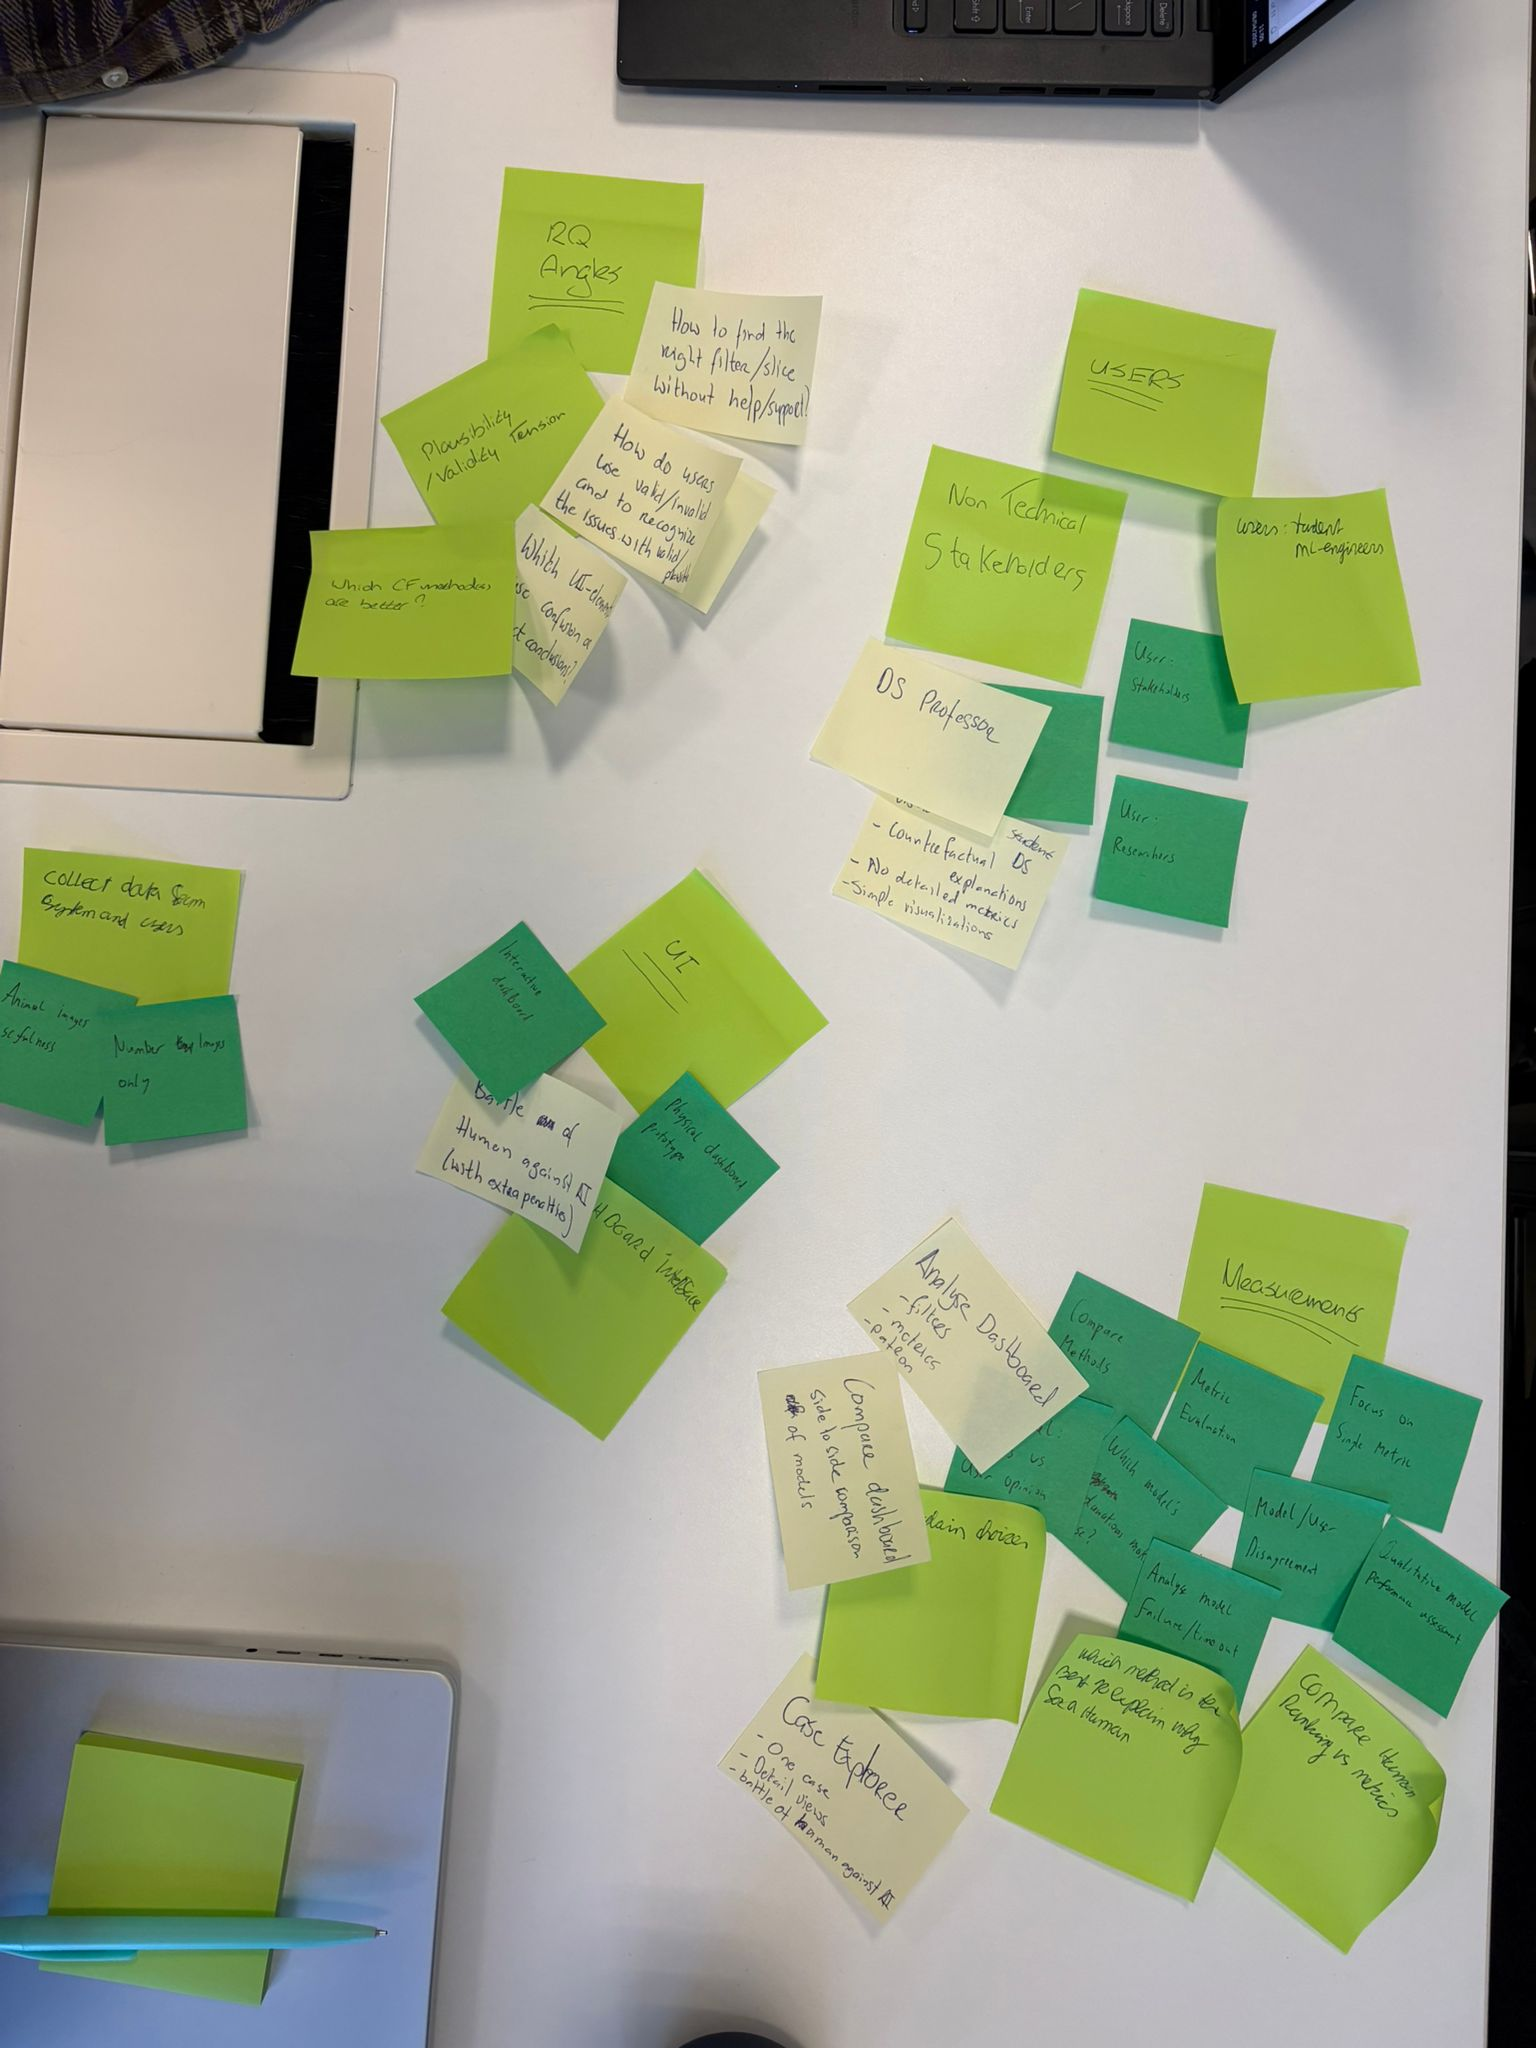
\includegraphics[width=4.6875in,height=\textheight,keepaspectratio]{images/ideation_1.jpeg}

}

\caption{Affinity mapping session showing early problem exploration and
user insights}

\end{figure}%

The workshop focused on three key areas:

\begin{enumerate}
\def\labelenumi{\arabic{enumi}.}
\tightlist
\item
  understanding how users interpret counterfactual explanations
\item
  identifying sources of confusion or misinterpretation
\item
  exploring potential use cases and interaction patterns
\end{enumerate}

The clustering process suggested several recurring themes. Many notes
pointed to the difficulty of determining which counterfactual
explanation is ``better,'' especially when multiple methods produce
different results. Other clusters indicated uncertainty about how to
interpret evaluation metrics and when these metrics can be trusted.

Importantly, this method surfaced both preliminary insights and open
questions, such as how users form judgments without guidance and whether
they rely more on visual intuition or numerical metrics.

\subsubsection{User Identification and Target Group
Definition}\label{user-identification-and-target-group-definition}

During the workshop, potential user groups were identified and refined.
The primary user group was defined as data science students, while
machine learning researchers were considered a secondary group.

\begin{figure}[H]

{\centering 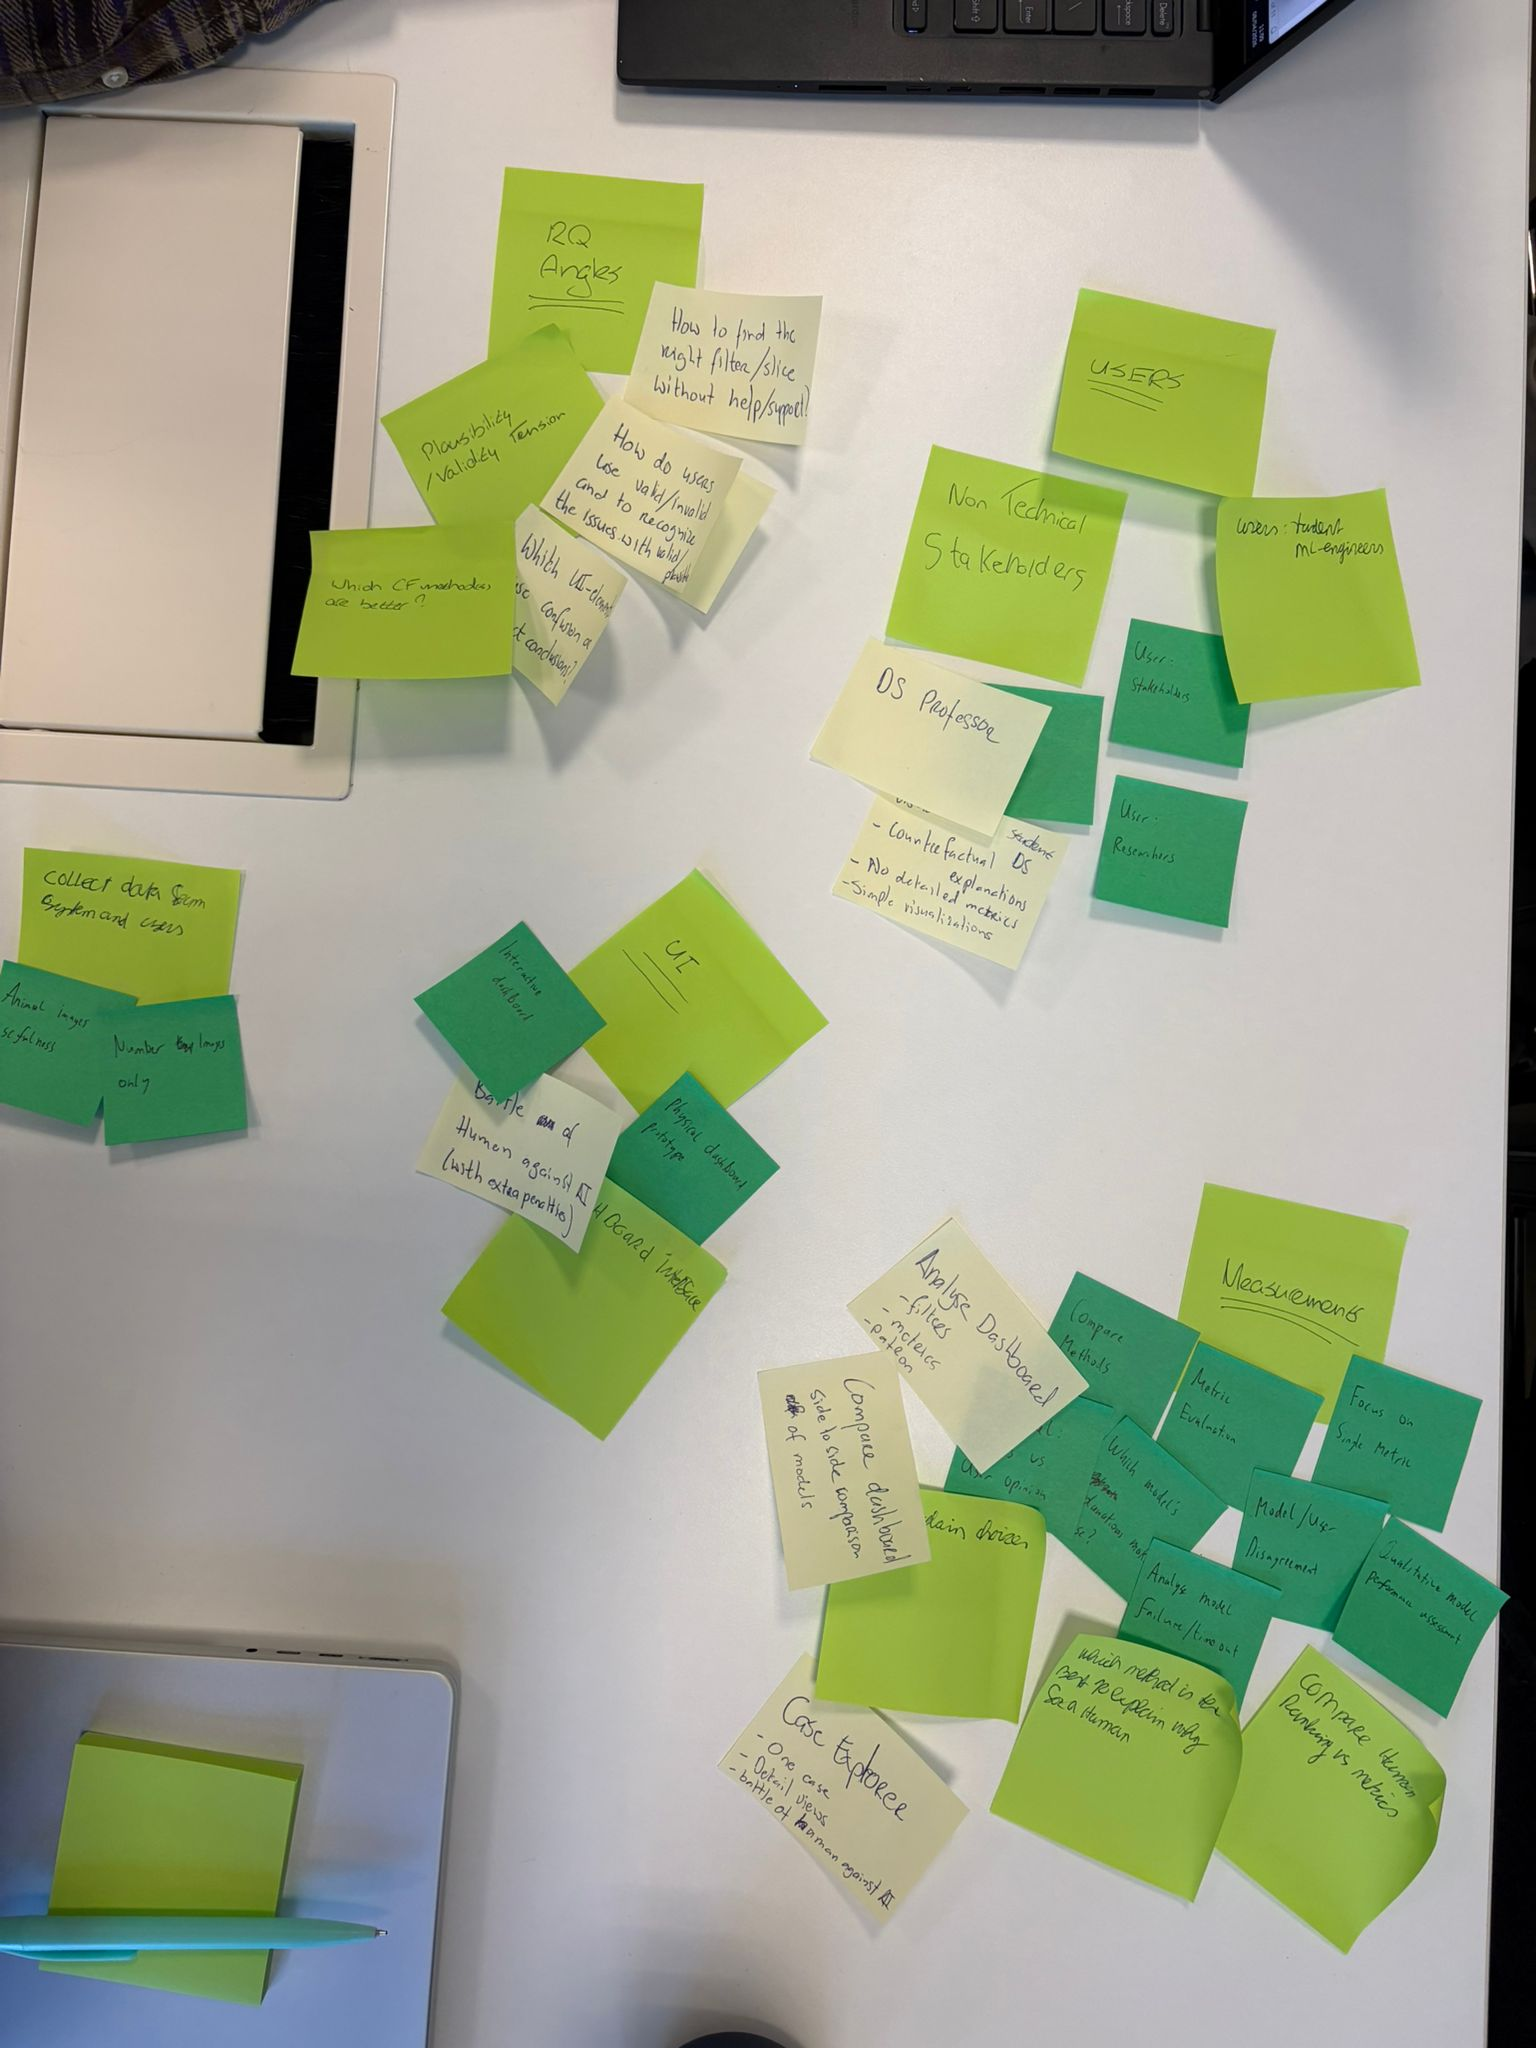
\includegraphics[width=4.54167in,height=\textheight,keepaspectratio]{images/ideation_2.jpeg}

}

\caption{User groups identified during the workshop}

\end{figure}%

Data science students are expected to have a basic understanding of
machine learning concepts but limited experience with evaluating
explanation quality. They may therefore rely more strongly on visual
intuition and may not fully understand the implications of different
evaluation metrics.

Machine learning researchers, in contrast, are more familiar with model
evaluation but may still face challenges when comparing multiple
explanation methods or interpreting trade-offs between different
metrics.

\subsubsection{Literature Scan}\label{literature-scan}

A targeted literature scan was conducted to contextualize the observed
challenges within existing research on explainable AI. Prior work
indicates that explanation quality is inherently multi-dimensional and
that no single metric fully captures what makes an explanation ``good''
(Guidotti et al. 2018).

Furthermore, research suggests that there can be a gap between objective
evaluation metrics and human interpretability. Doshi-Velez and Kim argue
that interpretability should be evaluated with respect to human
understanding, rather than purely technical criteria (Doshi-Velez and
Kim 2017).

In addition, studies on human interaction with explanation tools
indicate that users can be influenced by how information is presented.
For example, numerical metrics may lead to anchoring effects, where
users base their judgment on the metric rather than forming an
independent assessment (Kaur et al. 2020).

These findings provided a theoretical basis for interpreting the
workshop results.

\subsubsection{Technical Inspection of the
Dataset}\label{technical-inspection-of-the-dataset}

A technical inspection of the dataset was conducted by manually
exploring a subset of cases in which multiple counterfactual
explanations were generated for the same input instance. For each case,
the outputs of different methods were compared alongside their
associated evaluation metrics.

This inspection suggested that different methods can produce
substantially different counterfactuals for the same input. In several
observed cases, explanations that appeared visually plausible did not
achieve the intended target prediction, while other explanations that
were classified as valid by the model appeared less intuitive from a
human perspective.

These observations indicate that trade-offs between different evaluation
dimensions are present, and that explanation quality cannot be fully
captured by a single criterion.

\subsection{2.2 Results and Insights}\label{results-and-insights}

The combination of methods resulted in a set of key insights that
informed the subsequent design phases.

\subsubsection{Insight 1: Users struggle to distinguish validity from
plausibility}\label{insight-1-users-struggle-to-distinguish-validity-from-plausibility}

A central observation from the affinity mapping session is that users
have difficulty distinguishing between explanations that are technically
correct and those that appear visually convincing.

\begin{figure}

\centering{

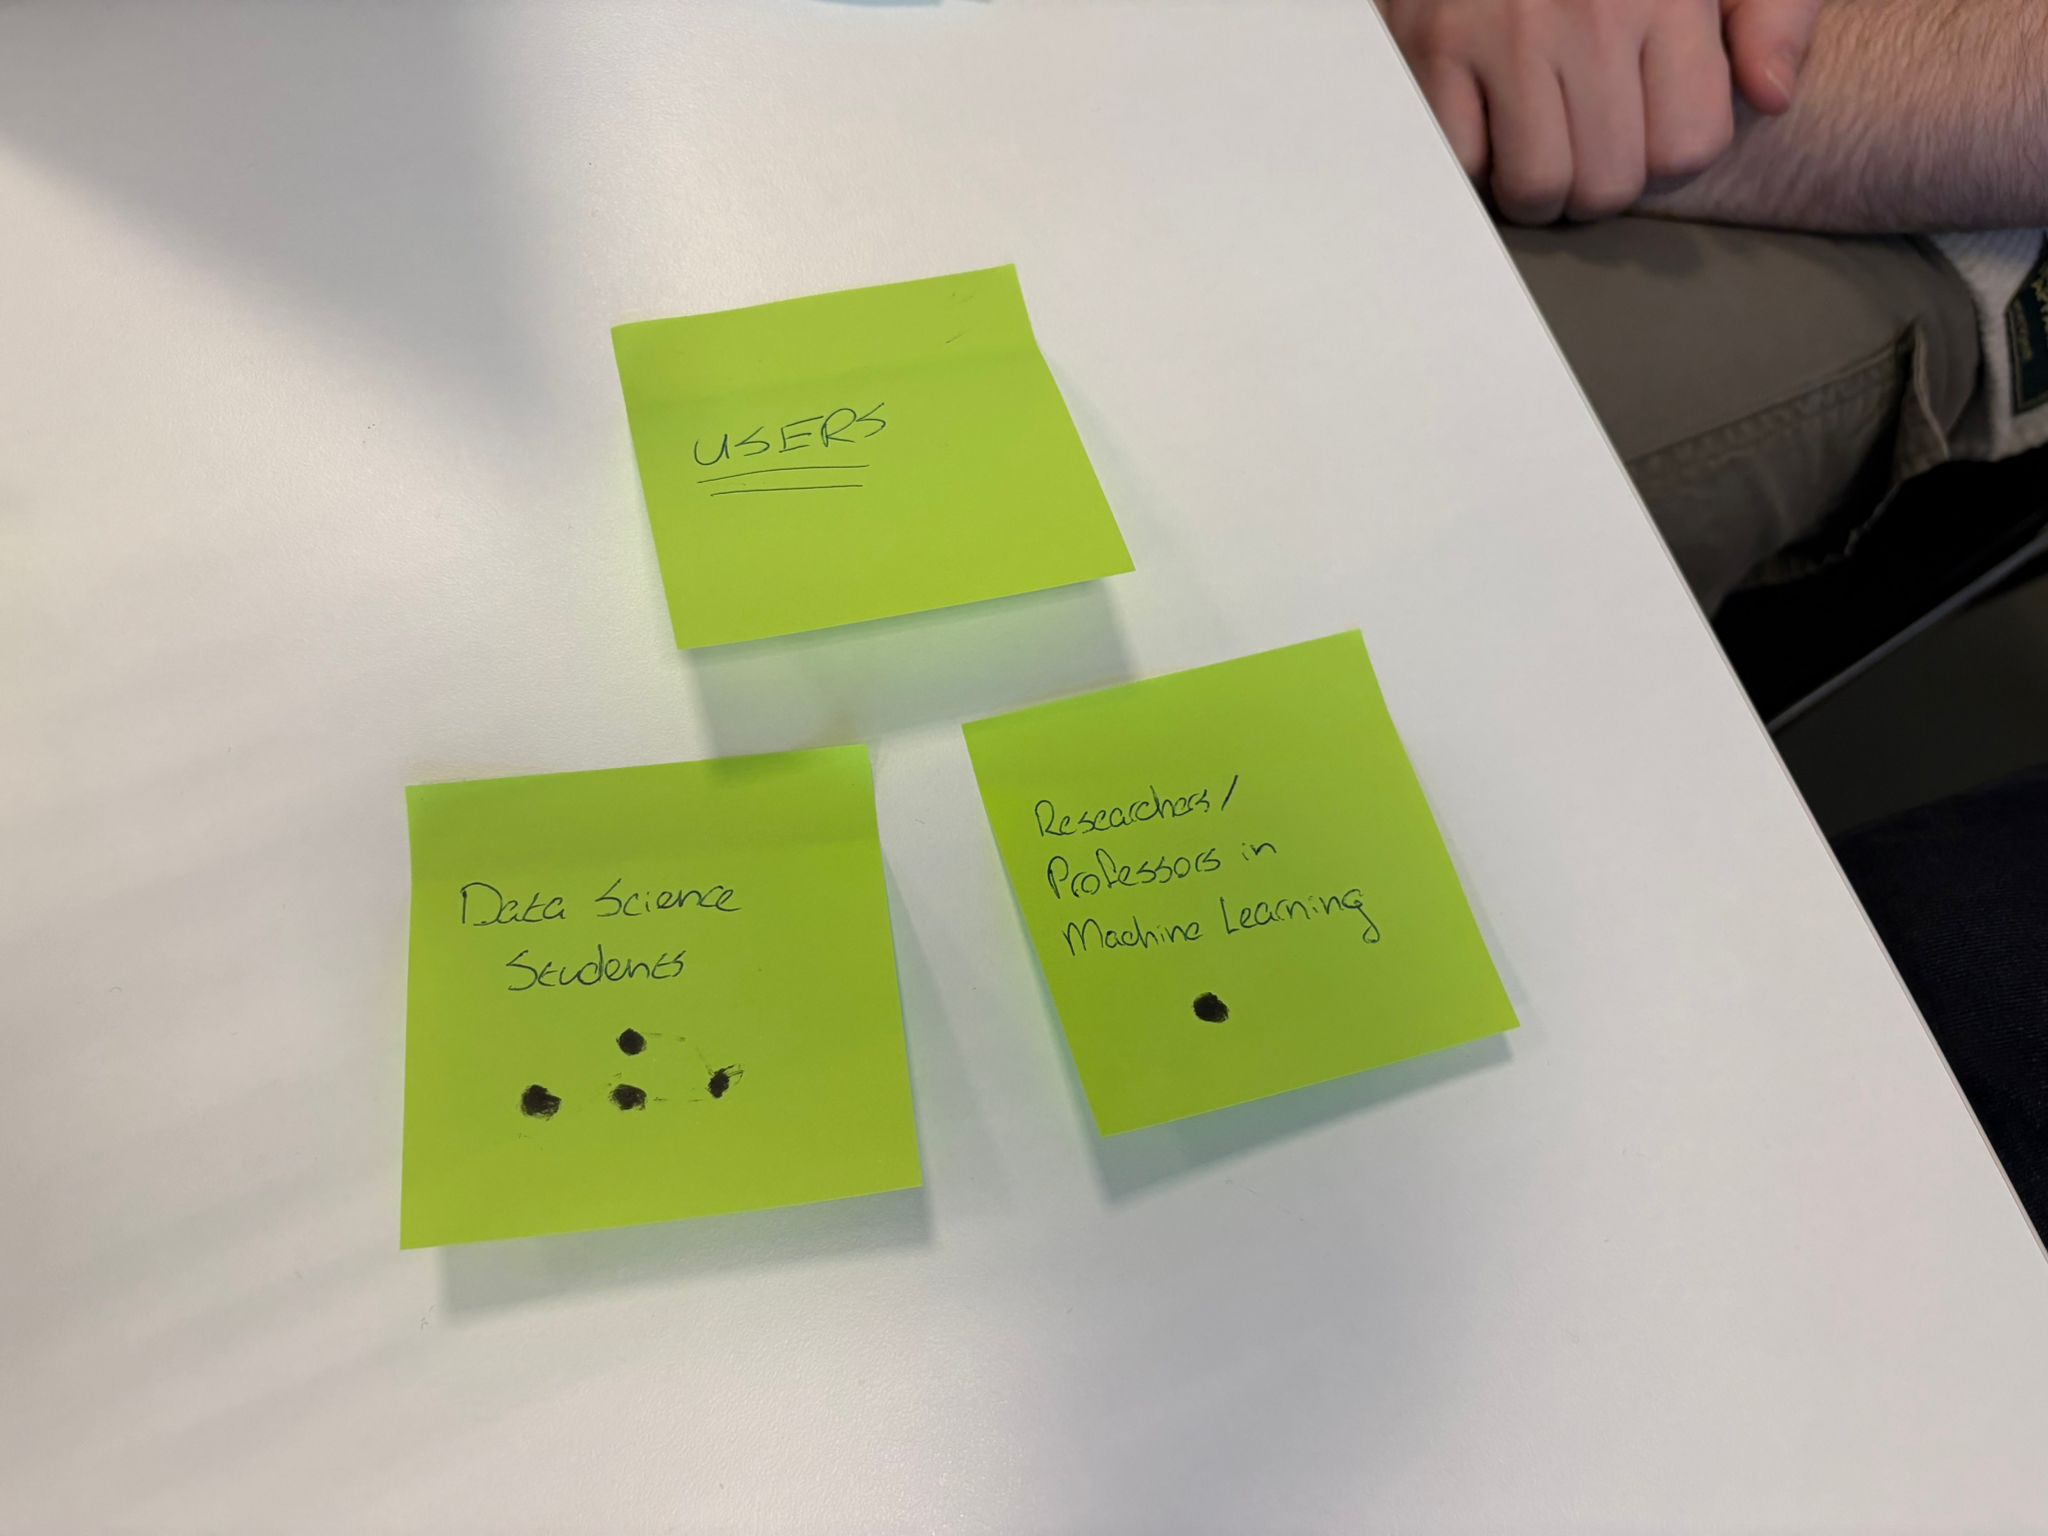
\includegraphics[width=4.5625in,height=\textheight,keepaspectratio]{images/ideation_3.jpeg}

}

\caption{\label{fig-brainwriting1}Clustering of insights related to
evaluation challenges}

\end{figure}%

Users tend to interpret explanations based on visual similarity or
perceived realism, rather than on whether the explanation actually
changes the model prediction. As a result, explanations that are valid
may be rejected, while implausible explanations may be accepted.

\subsubsection{Insight 2: Metrics can influence user
judgment}\label{insight-2-metrics-can-influence-user-judgment}

Another insight is that the presence of evaluation metrics can influence
how users interpret explanations.

\begin{figure}[H]

{\centering 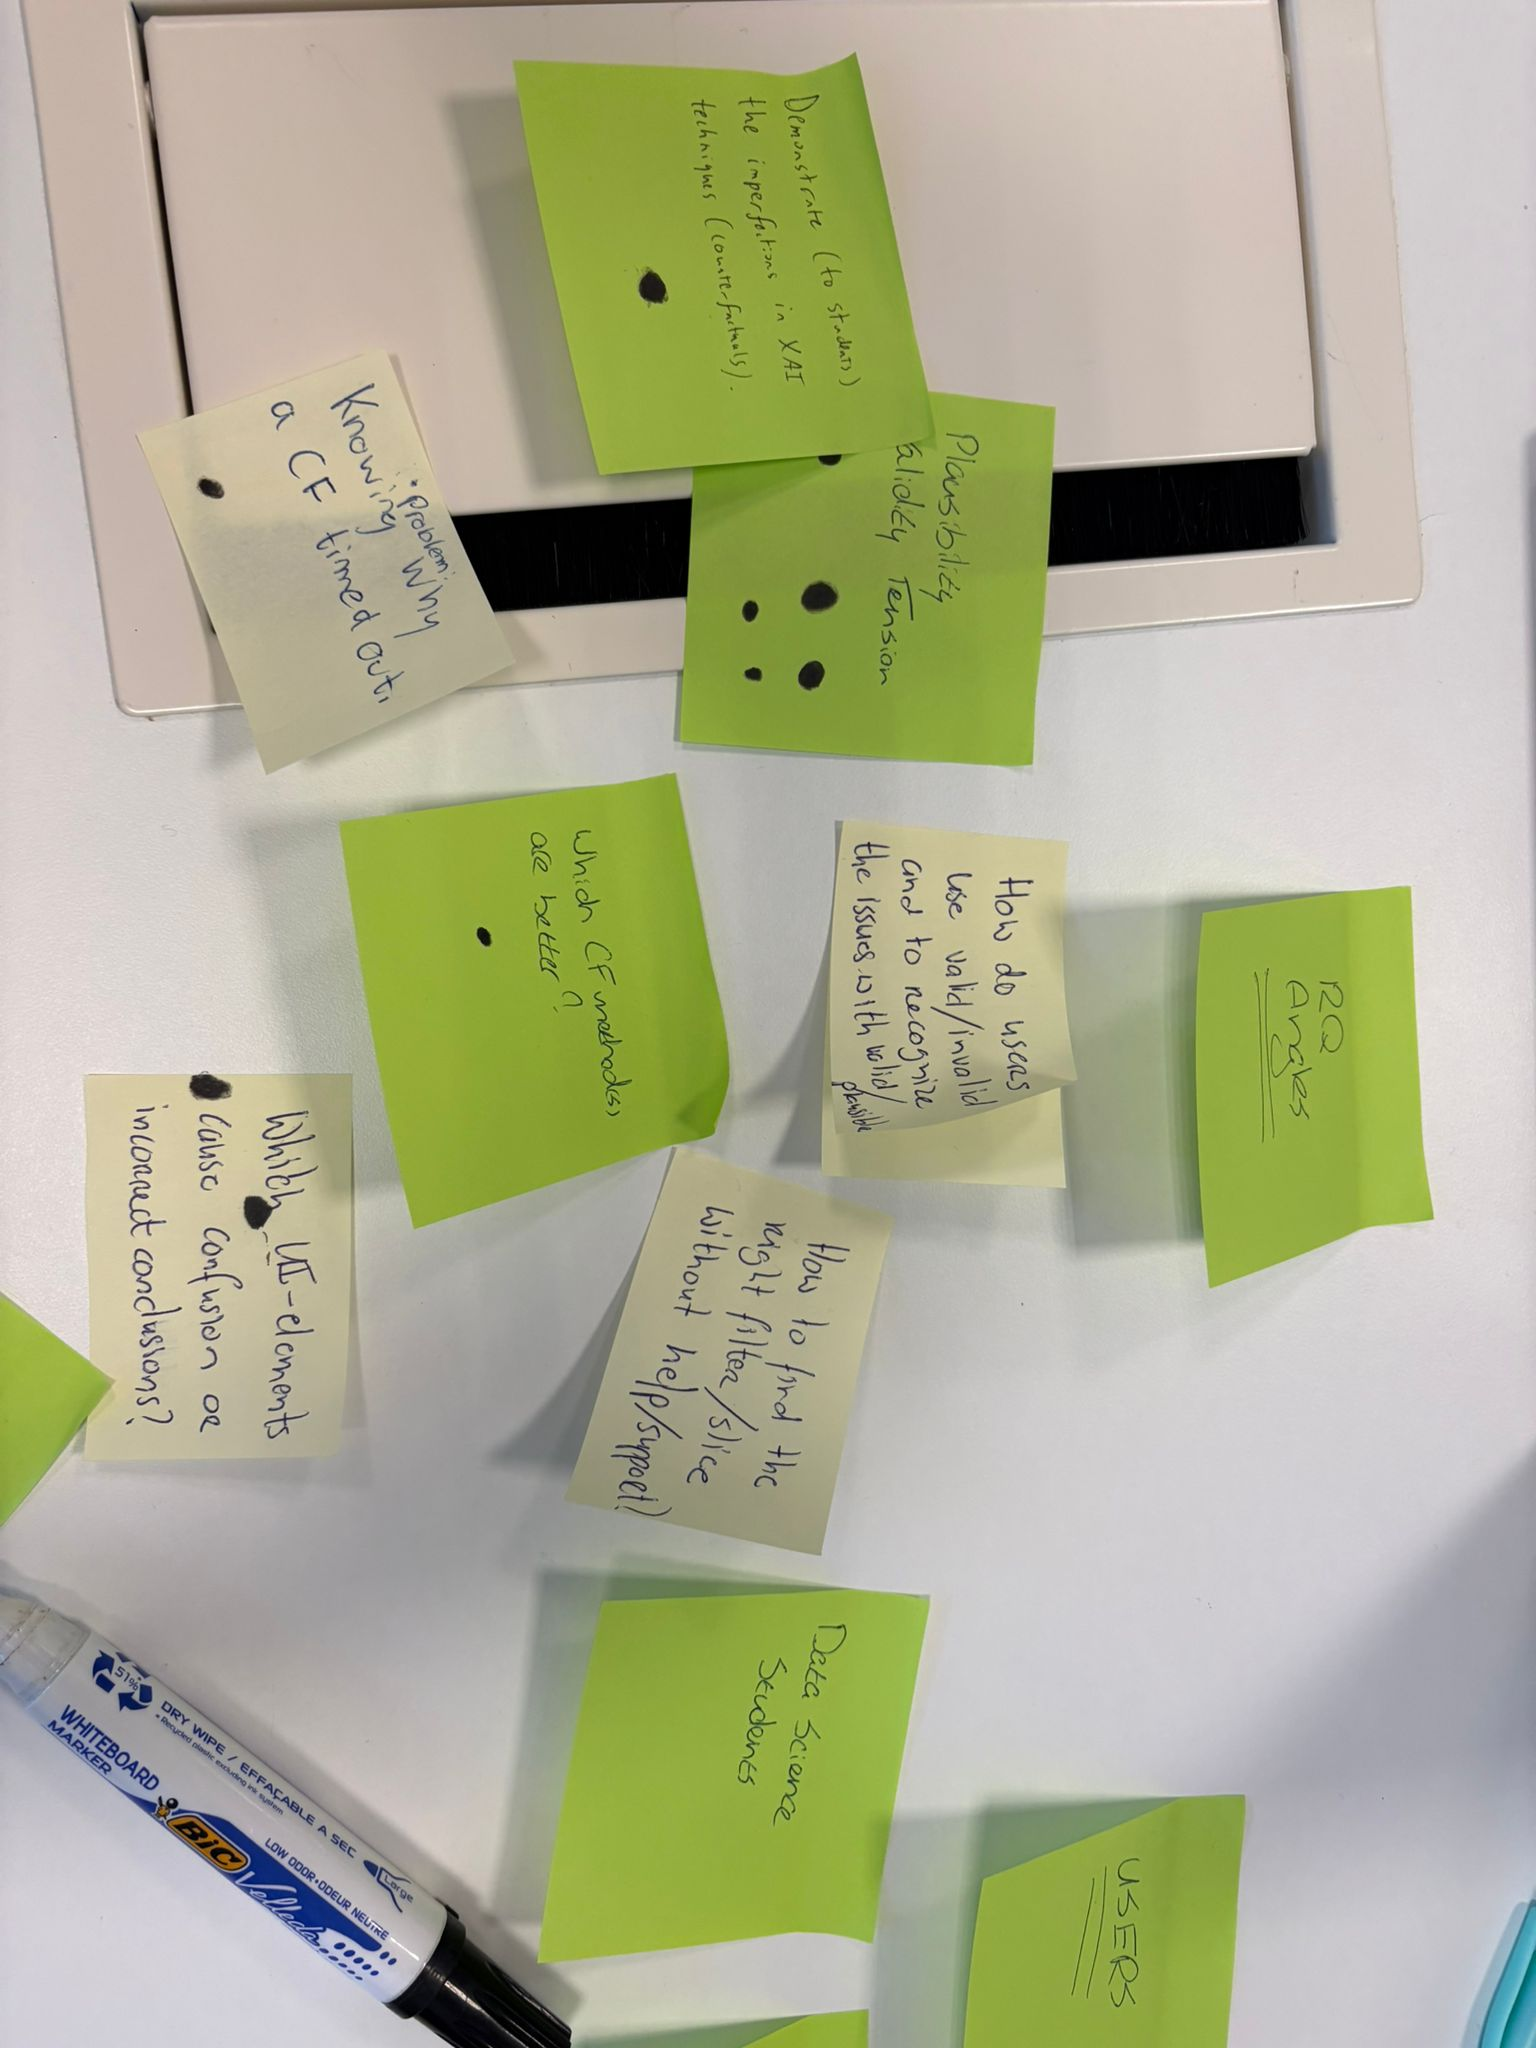
\includegraphics[width=4.55208in,height=\textheight,keepaspectratio]{images/ideation_4.jpeg}

}

\caption{Notes highlighting confusion and bias in interpretation}

\end{figure}%

Participants indicated that numerical values shown early in the process
may guide decision-making. Instead of forming an independent judgment,
users may rely on the metric as a heuristic, which can reduce critical
reflection.

\subsubsection{Insight 3: Comparing multiple explanations is cognitively
demanding}\label{insight-3-comparing-multiple-explanations-is-cognitively-demanding}

Users expressed difficulty in comparing multiple counterfactual
explanations simultaneously.

\begin{figure}[H]

{\centering 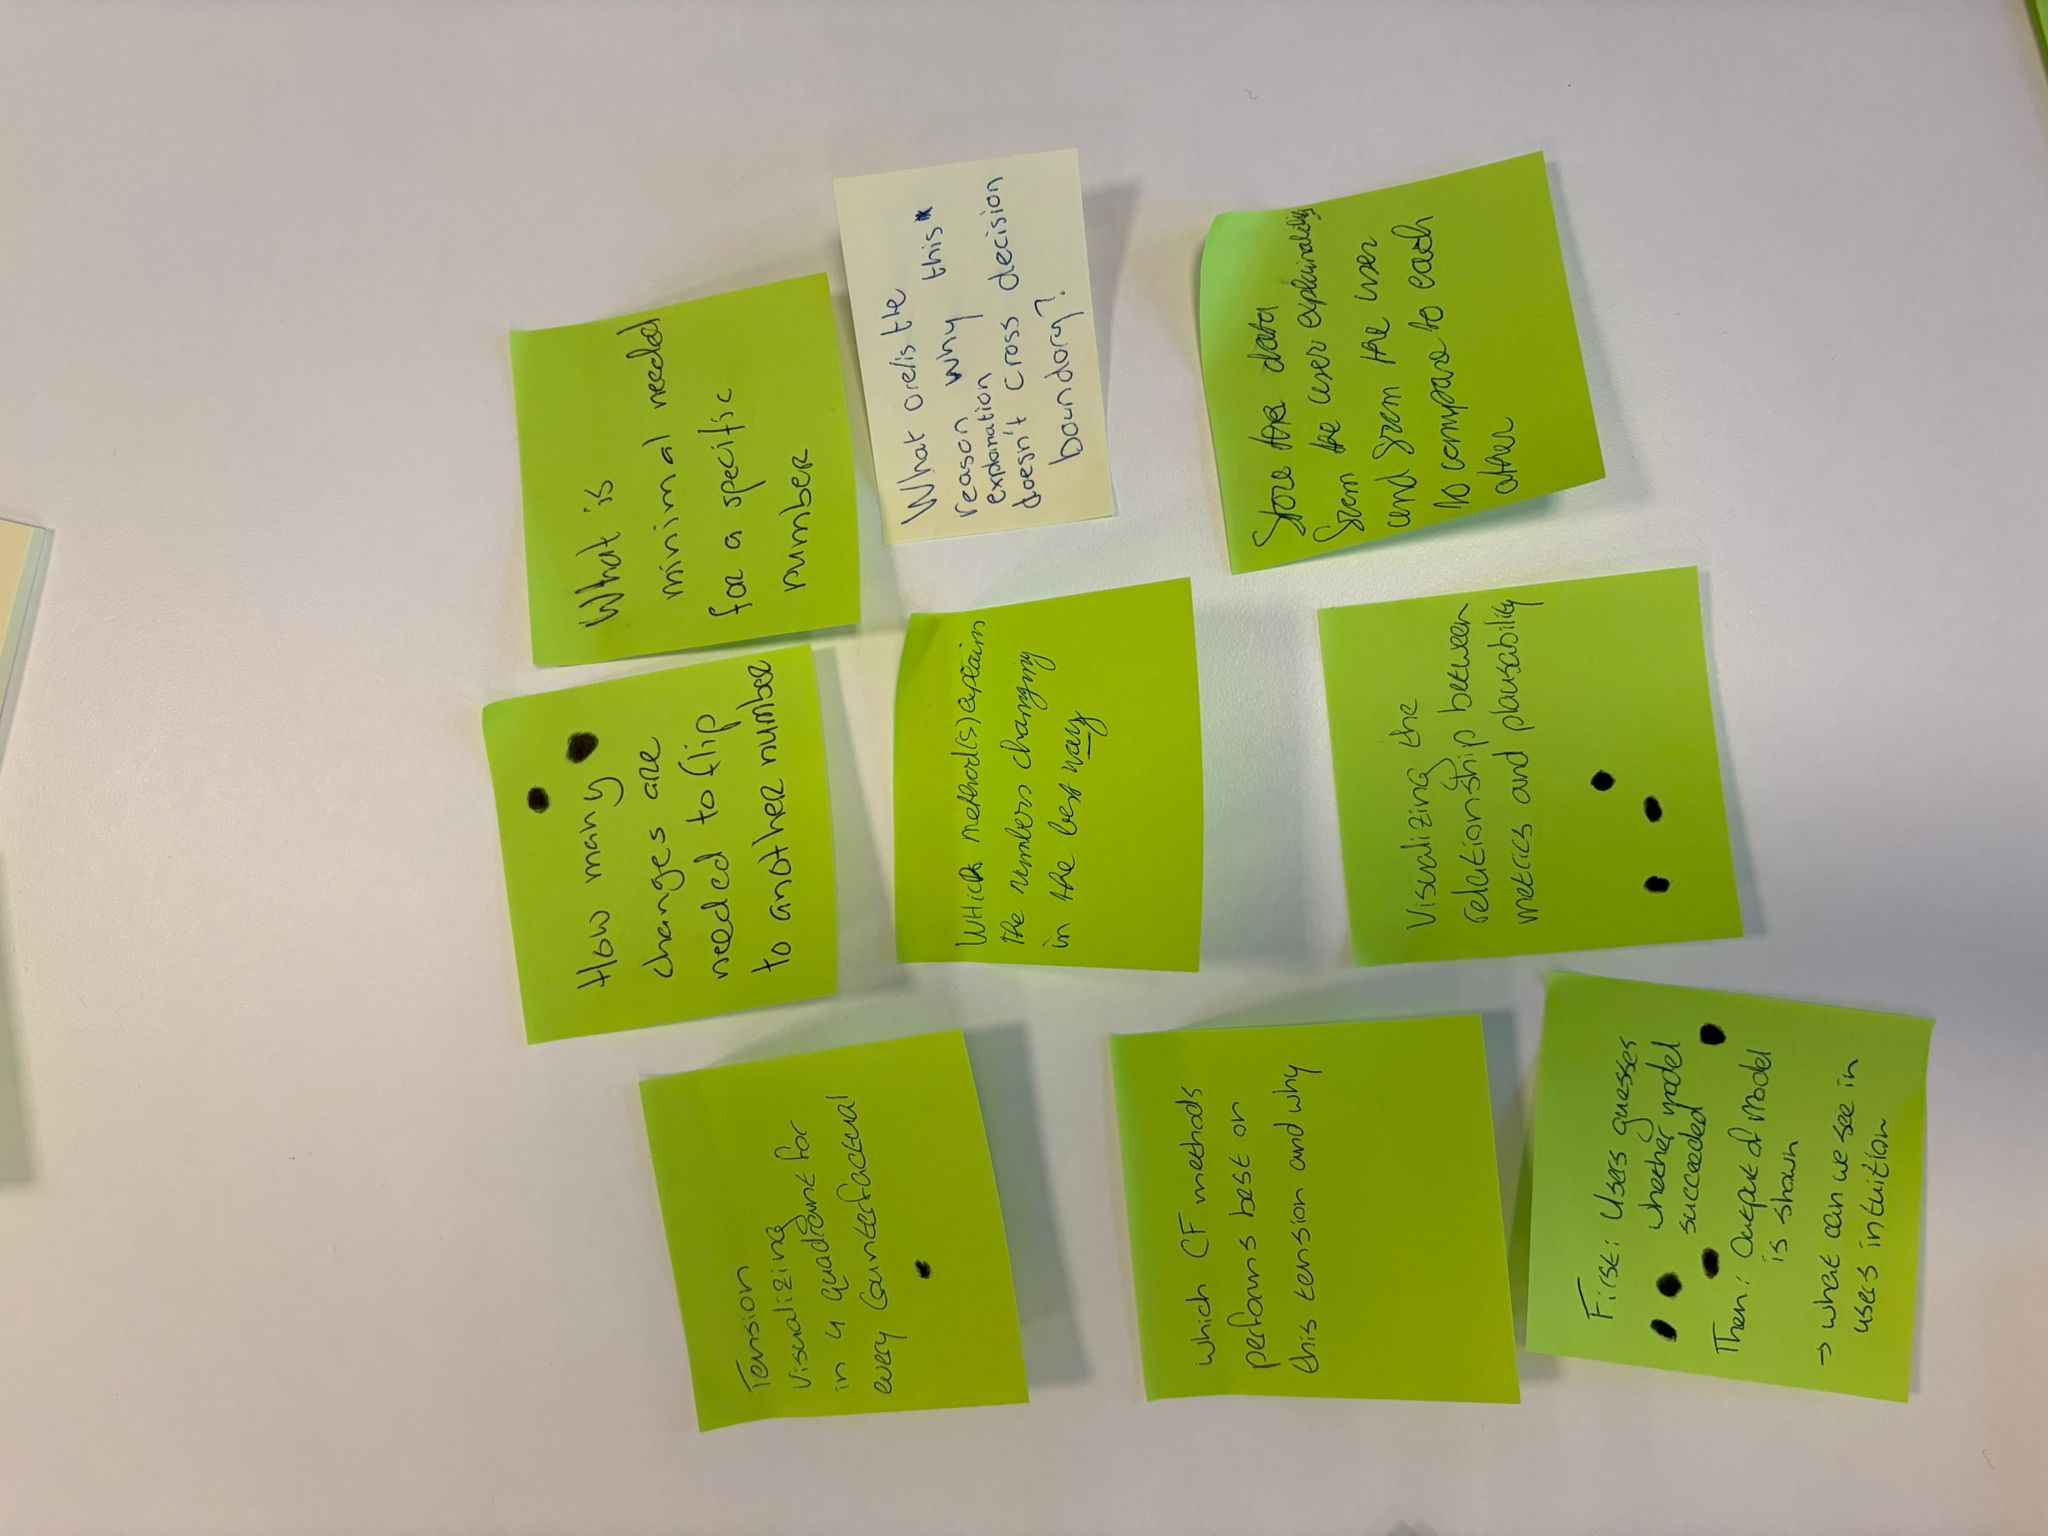
\includegraphics[width=4.67708in,height=\textheight,keepaspectratio]{images/ideation_5.jpeg}

}

\caption{Insights related to comparison and decision-making challenges}

\end{figure}%

The presence of multiple methods introduces several challenges:

\begin{itemize}
\tightlist
\item
  uncertainty about which criteria to use for comparison
\item
  difficulty in tracking differences between explanations
\item
  increased cognitive load when many options are presented
\end{itemize}

\subsubsection{Insight 4: The gap between intuition and metrics is not
explicit}\label{insight-4-the-gap-between-intuition-and-metrics-is-not-explicit}

An important insight is that the discrepancy between human intuition and
model-based evaluation is not explicitly represented in existing tools.

Users may form an initial judgment based on visual inspection, but this
judgment is typically not compared to objective metrics in a structured
way. As a result, potential misalignment remains implicit.

\subsubsection{Insight 5: Users benefit from structured
guidance}\label{insight-5-users-benefit-from-structured-guidance}

A final insight is that users may benefit from structured guidance when
interpreting explanations, rather than fully open exploration.

Without guidance, users may:

\begin{itemize}
\tightlist
\item
  focus on less relevant aspects of the explanation
\item
  misinterpret evaluation metrics
\item
  draw inconsistent conclusions
\end{itemize}

\subsection{2.3 Transition to Define
Phase}\label{transition-to-define-phase}

The empathize phase highlights a consistent pattern: users experience
difficulty interpreting counterfactual explanations, particularly due to
the misalignment between visual intuition and objective evaluation
metrics. This challenge is reinforced by the way information is
presented and by the complexity of comparing multiple explanations.

Based on these findings, the design focus is narrowed to the following
challenge:

\begin{tcolorbox}[enhanced jigsaw, opacityback=0, toprule=.15mm, colframe=quarto-callout-note-color-frame, colback=white, leftrule=.75mm, rightrule=.15mm, arc=.35mm, breakable, bottomrule=.15mm, left=2mm]
\begin{minipage}[t]{5.5mm}
\textcolor{quarto-callout-note-color}{\faInfo}
\end{minipage}%
\begin{minipage}[t]{\textwidth - 5.5mm}

How to design an interface that reveals and supports the interpretation
of the gap between human intuition and model-based evaluation.

\end{minipage}%
\end{tcolorbox}

This forms the basis for the define phase, where the problem will be
formalized into a clear problem statement.

\section{3 Define Phase}\label{define-phase}

\subsection{3.1 Problem Statement}\label{problem-statement}

The empathize phase revealed a consistent challenge: users experience
difficulty in interpreting counterfactual explanations due to the
misalignment between visual intuition and objective evaluation metrics.
While users tend to rely on visual similarity and perceived
plausibility, model-based metrics such as validity may indicate a
different assessment of explanation quality.

This leads to the following problem statement:

\begin{tcolorbox}[enhanced jigsaw, opacityback=0, toprule=.15mm, colframe=quarto-callout-note-color-frame, colback=white, leftrule=.75mm, rightrule=.15mm, arc=.35mm, breakable, bottomrule=.15mm, left=2mm]
\begin{minipage}[t]{5.5mm}
\textcolor{quarto-callout-note-color}{\faInfo}
\end{minipage}%
\begin{minipage}[t]{\textwidth - 5.5mm}

\emph{A data science student needs a way to systematically interpret and
compare counterfactual explanations, because current representations do
not make the relationship between human intuition and evaluation metrics
explicit, resulting in confusion and inconsistent judgments.}

\end{minipage}%
\end{tcolorbox}

This problem is directly grounded in the insights from the empathize
phase, where users expressed uncertainty about how to interpret metrics,
difficulty in comparing multiple explanations, and a tendency to rely on
intuition without validation.

\subsection{3.2 Target User}\label{target-user}

The primary target user for this project is a data science student.
These users typically have a foundational understanding of machine
learning models and evaluation concepts, but limited experience with
interpreting explanation quality, especially in situations where
multiple evaluation criteria are involved.

Data science students are likely to:

\begin{itemize}
\tightlist
\item
  rely on visual intuition when evaluating explanations
\item
  have difficulty interpreting abstract evaluation metrics
\item
  struggle to compare multiple counterfactual methods
\end{itemize}

A secondary user group consists of machine learning researchers. While
these users are more experienced with model evaluation, they may still
face challenges when comparing explanation methods or analysing
trade-offs between different evaluation criteria.

The design primarily focuses on supporting data science students, while
remaining relevant for more advanced users.

\subsection{3.3 Focus for Ideation}\label{focus-for-ideation}

Based on the insights from the empathize phase, the design focus is
narrowed to one central challenge: making the gap between human
intuition and model-based evaluation visible and interpretable.

This focus is derived from three key observations:

\begin{enumerate}
\def\labelenumi{\arabic{enumi}.}
\tightlist
\item
  Users struggle to distinguish between validity and plausibility
\item
  Evaluation metrics can influence or bias user judgment
\item
  Comparing multiple explanations introduces cognitive complexity
\end{enumerate}

These observations indicate that the core issue is not only the
availability of explanations, but how they are interpreted and compared.

Rather than designing a dashboard that prioritizes exploration or metric
visualization, the design will focus on structuring the interaction in
such a way that users first form an independent judgment, and only then
are confronted with model-based evaluation.

This leads to the following design direction:

\begin{itemize}
\tightlist
\item
  guide users through a step-by-step evaluation process
\item
  separate intuition from metric-based evaluation
\item
  explicitly compare user judgments with model outputs
\end{itemize}

This direction forms the basis for the ideation phase, where multiple
design concepts will be explored to determine how such a guided
interaction can be implemented effectively.

\section{4 Ideation Phase}\label{ideation-phase}

\subsection{4.1 Divergence --- Generating Design
Concepts}\label{divergence-generating-design-concepts}

Following the define phase, the ideation phase focused on exploring a
broad range of possible solutions to address the central challenge:
\emph{making the gap between human intuition and model-based evaluation
visible and interpretable}.

To ensure sufficient divergence, a structured brainwriting session was
conducted. Each team member independently generated ideas before sharing
them with the group. This approach reduced the risk of early convergence
on familiar solutions and encouraged the exploration of alternative
interaction patterns.

\begin{figure}

\centering{

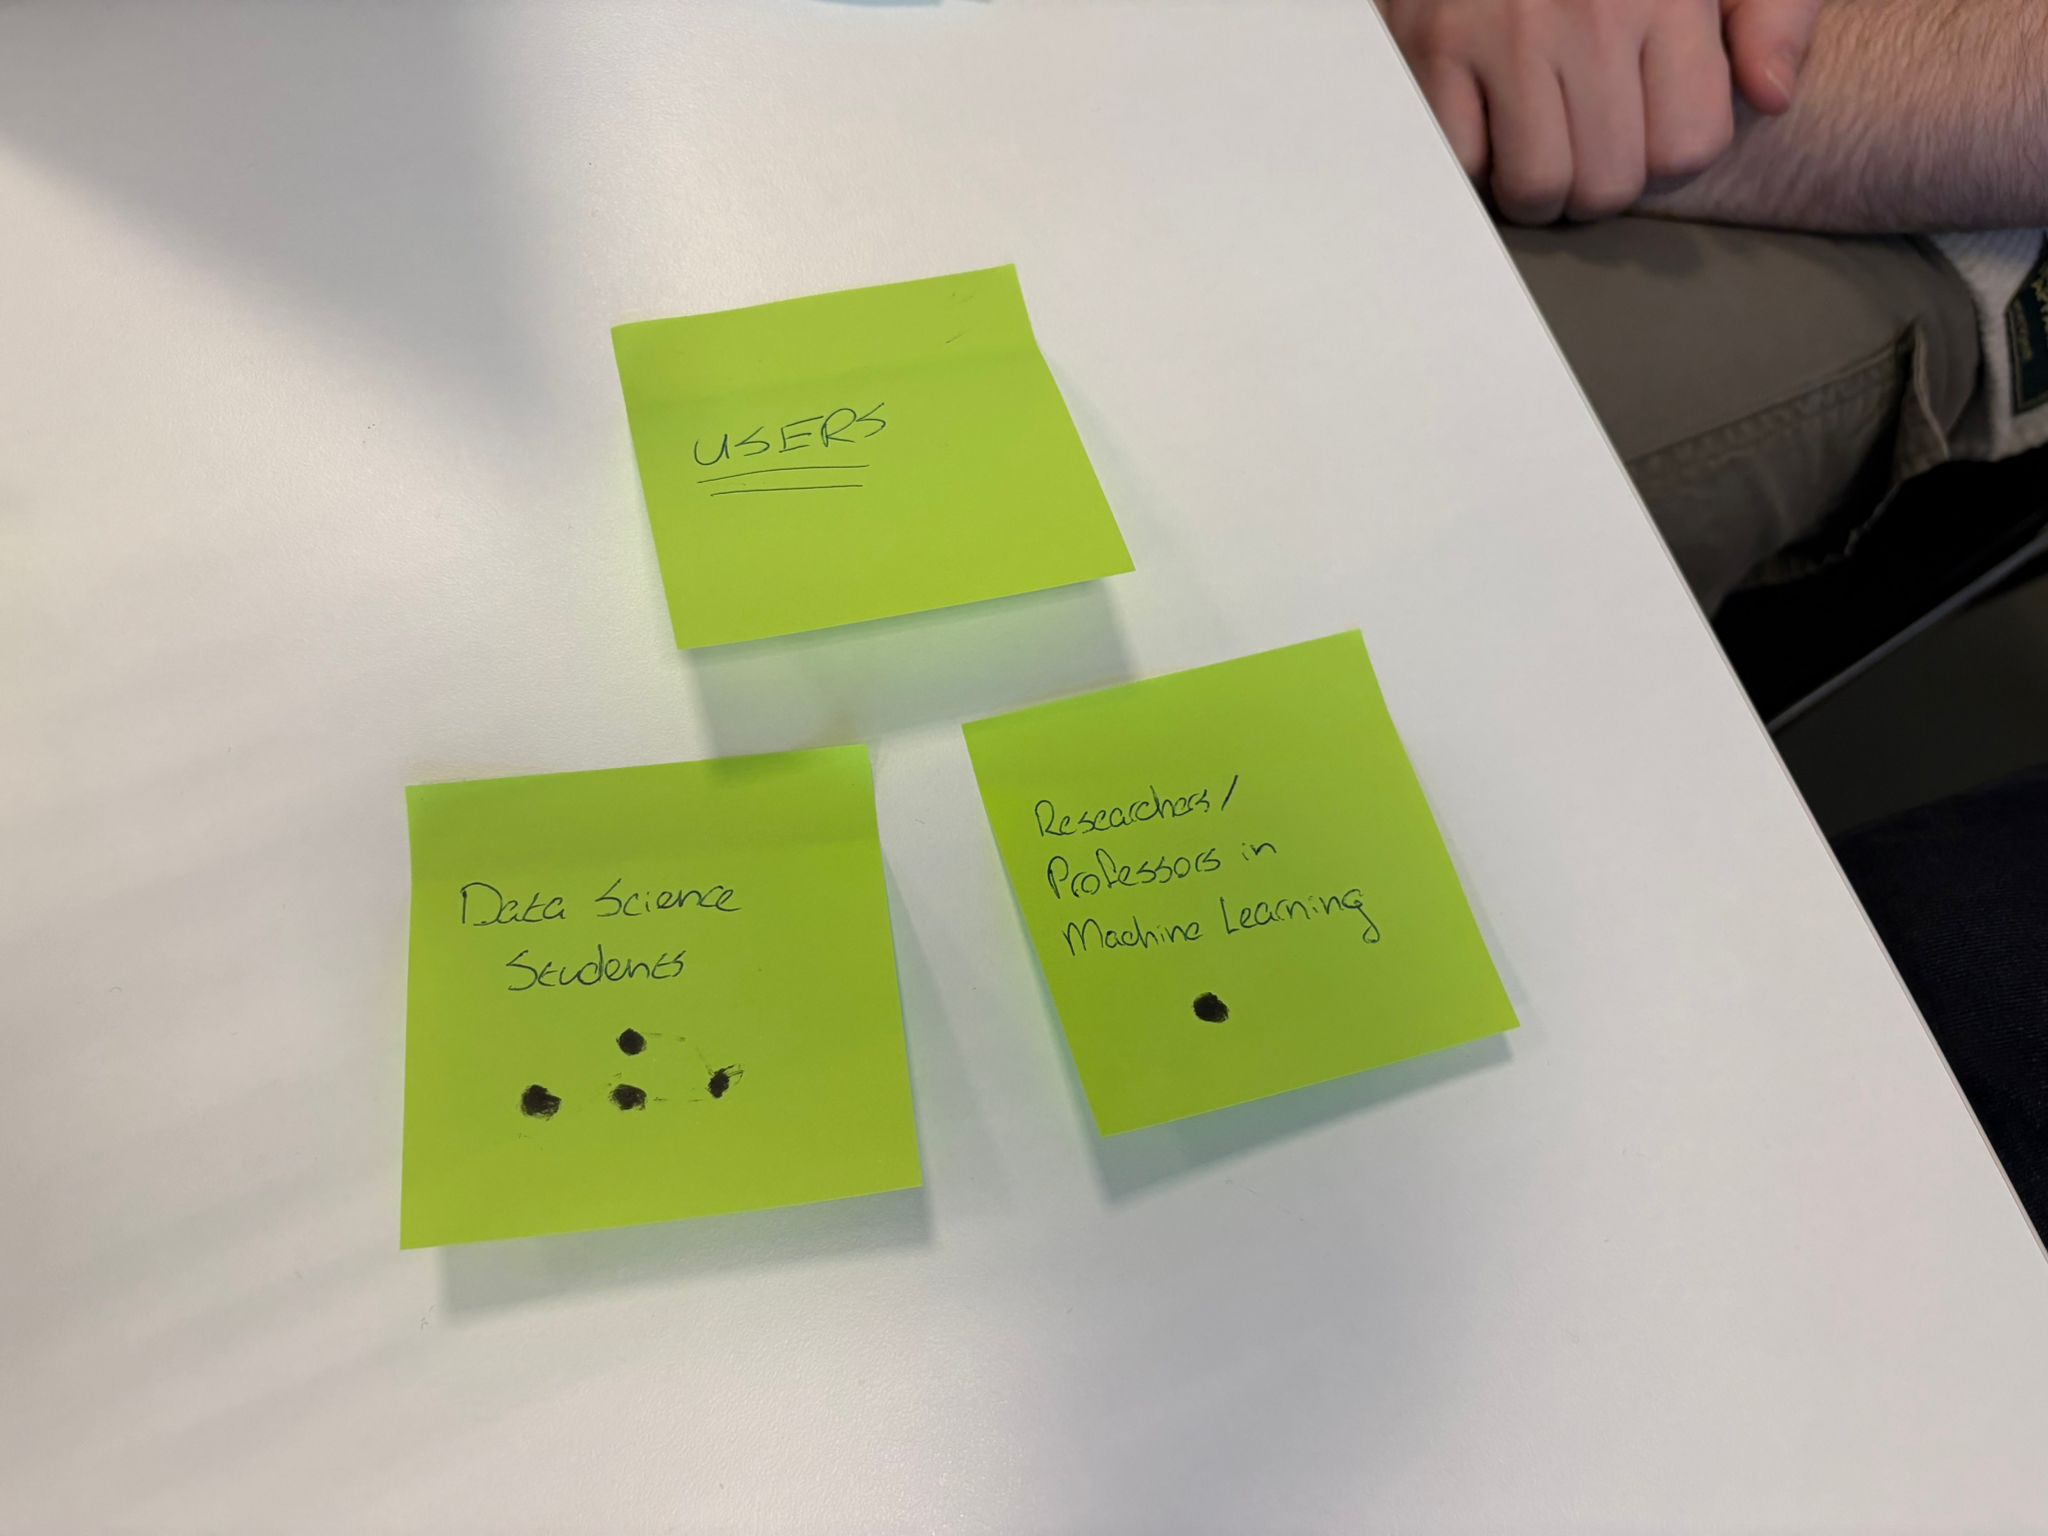
\includegraphics[width=4.71875in,height=\textheight,keepaspectratio]{images/ideation_3.jpeg}

}

\caption{\label{fig-brainwriting2}Brainwriting session showing a wide
range of alternative dashboard concepts}

\end{figure}%

Figure Figure~\ref{fig-brainwriting2} illustrates the divergence phase.
The variety of post-it notes reflects multiple directions, including
dashboard-based exploration, metric-driven evaluation, comparison views,
and more structured interaction flows.

Ideas were intentionally not evaluated during the initial generation
phase. This allowed both conventional and more experimental concepts to
emerge before introducing selection criteria.

The generated ideas can be grouped into several concept categories.

\subsubsection{Free Exploration
Dashboard}\label{free-exploration-dashboard}

One concept focused on a traditional dashboard approach, where users can
freely explore counterfactual explanations using filters, dropdowns, and
coordinated visualizations.

Strengths:

\begin{itemize}
\tightlist
\item
  Supports flexible exploration and user control
\item
  Aligns with familiar dashboard interaction patterns
\item
  Allows users to define their own analysis process
\end{itemize}

Limitations:

\begin{itemize}
\tightlist
\item
  Requires users to determine their own evaluation strategy
\item
  Does not reduce cognitive load when comparing multiple explanations
\item
  Offers limited support for interpreting evaluation metrics
\end{itemize}

Relation to the core problem: This concept does not explicitly address
the gap between intuition and model-based evaluation. It assumes that
users are able to interpret explanations independently, which
contradicts the findings from the empathize phase.

\subsubsection{Metric-First Evaluation
Interface}\label{metric-first-evaluation-interface}

Another concept prioritized evaluation metrics as the primary entry
point. Users would first see values such as validity and plausibility,
and then inspect the corresponding counterfactual explanations.

Strengths:

\begin{itemize}
\tightlist
\item
  Supports systematic and metric-driven evaluation
\item
  Makes quantitative differences between methods explicit
\item
  Efficient for expert users
\end{itemize}

Limitations:

\begin{itemize}
\tightlist
\item
  Risks influencing user judgment through anchoring effects
\item
  Reduces the role of independent interpretation
\item
  May discourage critical reflection
\end{itemize}

Relation to the core problem: This concept potentially reinforces the
misalignment between intuition and metrics by prioritizing numerical
values over user interpretation. It therefore does not support the goal
of making this gap visible.

\subsubsection{Explanation Comparison
View}\label{explanation-comparison-view}

A third concept focused on side-by-side comparison of multiple
counterfactual explanations.

\begin{figure}

\centering{

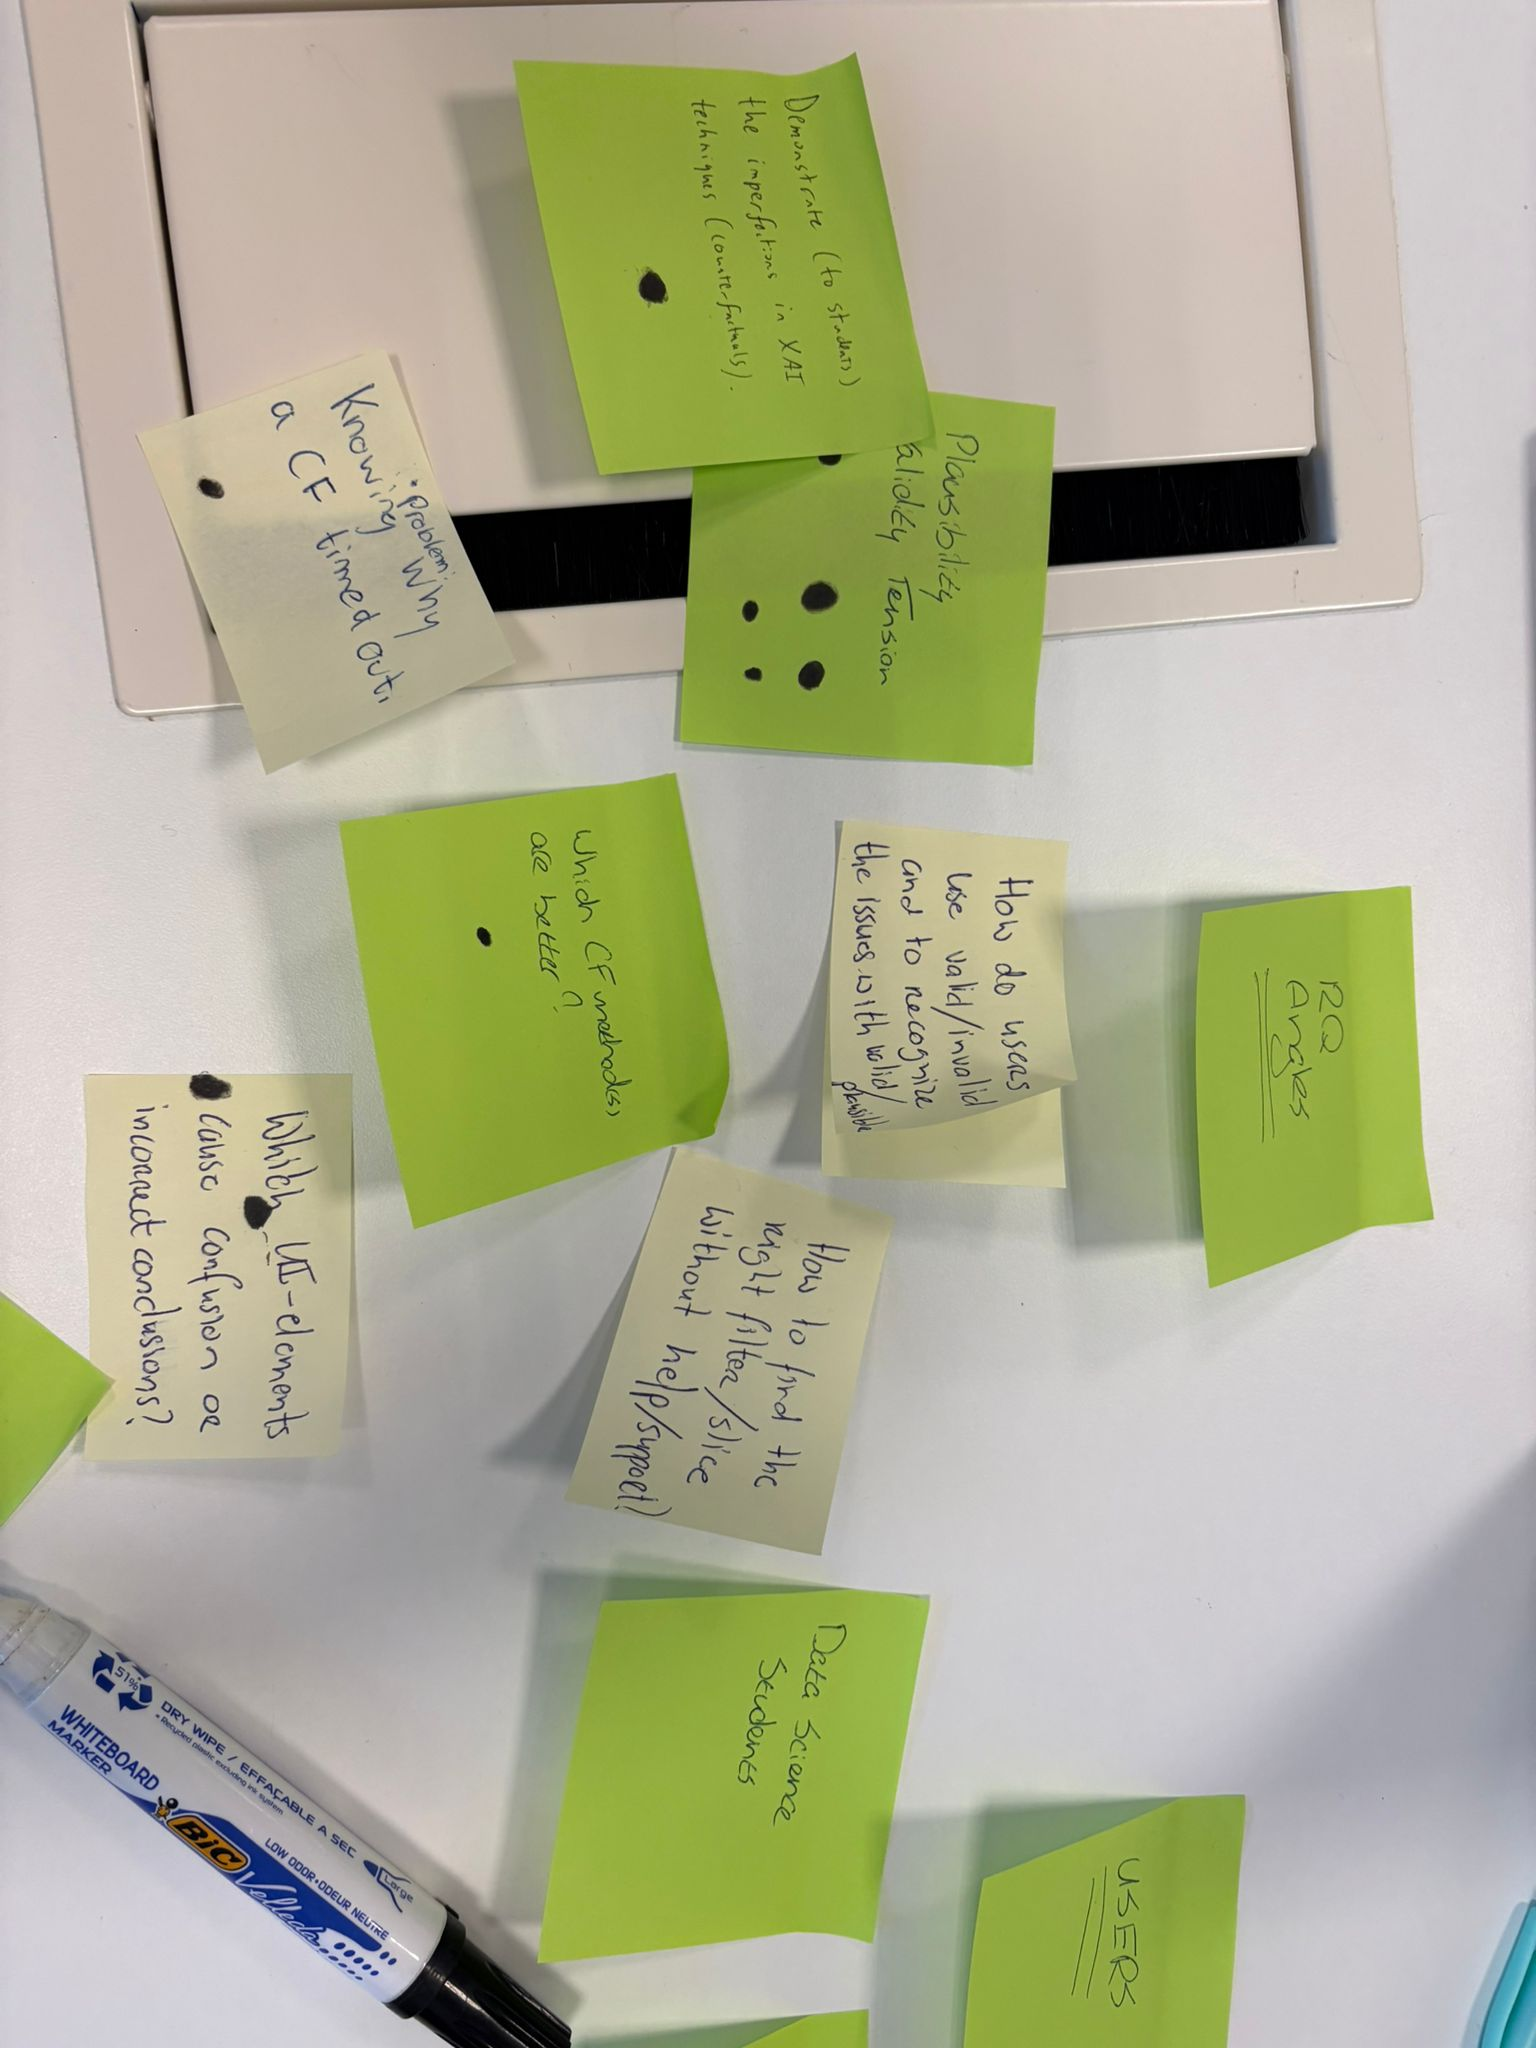
\includegraphics[width=4.23958in,height=\textheight,keepaspectratio]{images/ideation_4.jpeg}

}

\caption{\label{fig-patterns}Generated ideas focusing on interaction
patterns and evaluation challenges}

\end{figure}%

Strengths:

\begin{itemize}
\tightlist
\item
  Enables direct comparison between different methods
\item
  Makes visual differences between explanations observable
\item
  Supports exploratory analysis
\end{itemize}

Limitations:

\begin{itemize}
\tightlist
\item
  Introduces cognitive load when multiple explanations are presented
\item
  Does not provide guidance on how to evaluate differences
\item
  Leaves interpretation strategy undefined
\end{itemize}

Relation to the core problem:\\
While this concept supports comparison, it does not explicitly structure
the relationship between intuition and metrics. Users are still required
to interpret both independently.

\subsubsection{Ranking-Based Interface}\label{ranking-based-interface}

Another idea involved automatically ranking counterfactual explanations
based on selected metrics.

Strengths:

\begin{itemize}
\tightlist
\item
  Reduces decision effort for users
\item
  Provides a clear outcome based on defined criteria
\item
  Supports quick identification of ``best'' explanations
\end{itemize}

Limitations:

\begin{itemize}
\tightlist
\item
  Removes the need for user interpretation
\item
  Obscures trade-offs between different metrics
\item
  Does not expose disagreement between human judgment and model
  evaluation
\end{itemize}

Relation to the core problem:\\
This concept bypasses the central issue by replacing user judgment with
automated ranking. As a result, it does not support the investigation of
discrepancies between intuition and metrics.

\subsubsection{Guided Task Mode}\label{guided-task-mode}

The final concept introduced a structured interaction flow in which
users are guided through a sequence of evaluation steps.

In this concept, users:

\begin{enumerate}
\def\labelenumi{\arabic{enumi}.}
\tightlist
\item
  evaluate explanations based on visual inspection
\item
  estimate evaluation metrics
\item
  are presented with actual model metrics
\item
  reflect on differences between their judgment and the model output
\end{enumerate}

Strengths:

\begin{itemize}
\tightlist
\item
  Structures the evaluation process
\item
  Separates intuition from metric-based evaluation
\item
  Enables direct comparison between user input and model output
\item
  Reduces cognitive load through step-by-step interaction
\end{itemize}

Limitations:

\begin{itemize}
\tightlist
\item
  Less flexible than free exploration dashboards
\item
  Requires careful design to avoid over-guidance
\end{itemize}

Relation to the core problem:\\
This concept directly addresses the central challenge by making the
relationship between intuition and metrics explicit. It operationalizes
the gap identified in the empathize phase and creates a measurable
interaction.

\subsection{4.2 COCD Box --- Structuring Divergence and
Convergence}\label{cocd-box-structuring-divergence-and-convergence}

To support convergence, the generated ideas were mapped onto a COCD
(Creative Problem Solving) box, positioning them based on feasibility
and originality.

\begin{figure}[H]

{\centering \pandocbounded{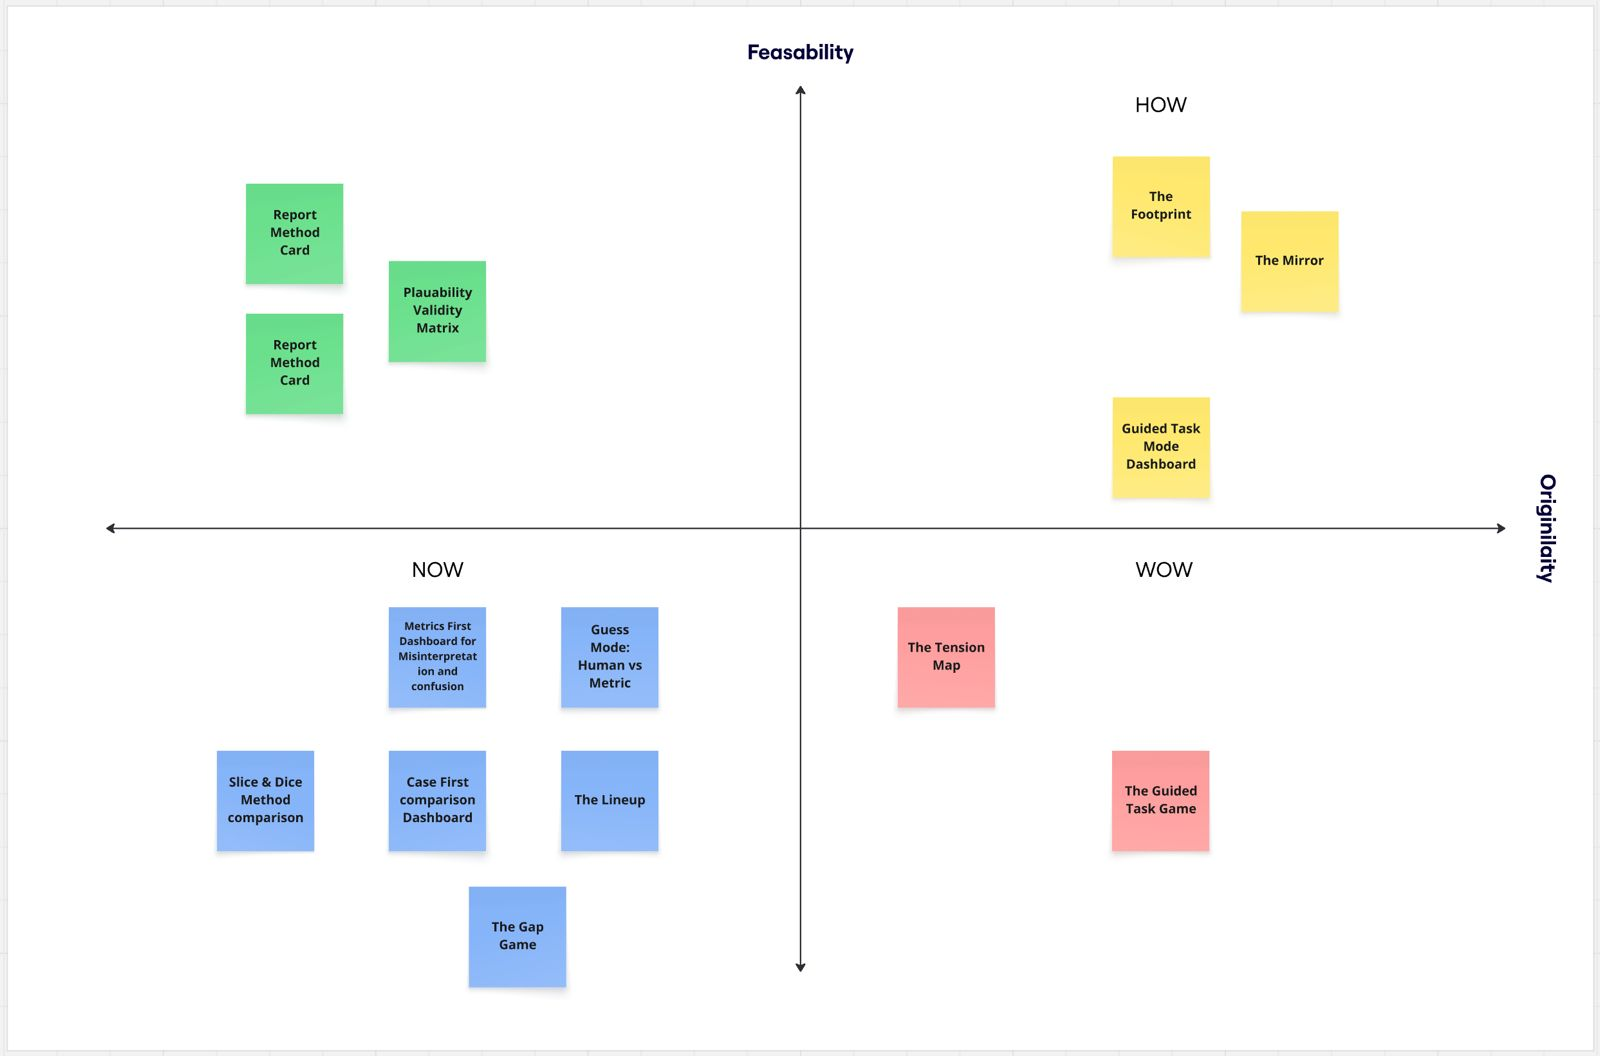
\includegraphics[keepaspectratio]{images/COCD.jpeg}}

}

\caption{COCD box showing divergence and convergence of design ideas}

\end{figure}%

The COCD box distinguishes four quadrants:

\begin{itemize}
\tightlist
\item
  Now: high feasibility, low originality
\item
  How: high feasibility, higher originality
\item
  Wow: high originality, lower feasibility
\item
  Non-ideas: low feasibility and low relevance
\end{itemize}

Most ideas were positioned in the ``Now'' quadrant, including
\emph{Metrics First Dashboard}, \emph{Case First Comparison Dashboard},
\emph{Slice \& Dice Method Comparison}, \emph{The Lineup}, and \emph{The
Gap Game}. These concepts are feasible and align with established design
patterns, but do not fundamentally change how users interpret
explanations.

Several concepts were positioned in the ``How'' quadrant, including
\emph{The Footprint}, \emph{The Mirror}, and the \emph{Guided Task Mode
Dashboard}. These ideas introduce new interaction patterns while
remaining feasible within the scope of the project.

Two concepts, \emph{The Tension Map} and \emph{The Guided Task Game},
were placed in the ``Wow'' quadrant. While these ideas offer high
originality, they were considered less feasible to implement within the
available time constraints.

The distribution of ideas indicates that initial ideation tended to
gravitate toward familiar solutions. The COCD mapping made it possible
to explicitly identify and select concepts that introduce meaningful
innovation while remaining implementable.

\subsection{4.3 Convergence --- Selection of Design
Direction}\label{convergence-selection-of-design-direction}

Based on the COCD analysis and the insights from the empathize and
define phases, the \emph{Guided Task Mode Dashboard} was selected as the
primary design direction.

This decision is based on three considerations.

\subsubsection{Alignment with User
Needs}\label{alignment-with-user-needs}

The guided task mode addresses the observed difficulties in interpreting
counterfactual explanations by structuring the evaluation process. It
reduces cognitive complexity and supports users in forming judgments
step by step.

Unlike free exploration approaches, it provides guidance without
removing user agency.

\subsubsection{Mitigating Metric Bias}\label{mitigating-metric-bias}

The empathize phase highlighted the risk of metric-driven bias. The
guided task mode addresses this by delaying the presentation of
evaluation metrics.

Users first form an independent judgment, after which they are exposed
to model-based evaluation. This supports a clearer distinction between
intuition and metrics.

\subsubsection{Making the Core Problem
Observable}\label{making-the-core-problem-observable}

The guided task mode makes the central problem measurable. By capturing
both user judgments and model outputs, it enables the analysis of
discrepancies between the two.

Alternative concepts either prioritize exploration or automate
evaluation, but do not make this relationship explicit.

\subsection{4.4 Design Direction}\label{design-direction}

The selected design direction can be summarized as follows:

\begin{itemize}
\tightlist
\item
  a step-by-step interaction flow that guides users through evaluation
  tasks
\item
  separation between intuitive judgment and metric-based evaluation
\item
  explicit comparison between user input and model output
\item
  structured reflection on discrepancies
\end{itemize}

This direction ensures that the design is directly aligned with the
research question and provides a clear foundation for the prototype
phase, where the guided interaction is translated into a concrete
interface.

\section{Prototype Phase}\label{prototype-phase}

\subsection{Prototype Description}\label{prototype-description}

The prototype is an interactive web-based dashboard built with
Streamlit, designed to serve two types of users: \textbf{study
participants} (data science students who evaluate counterfactual
explanations) and \textbf{researchers} (who collect and analyse the
resulting data). The dashboard runs on real data, PyTorch image tensors
generated by five CF methods across 1 dataset (MNIST) and supports
genuine interaction at every step, making it appropriate for a real user
study rather than a demonstration.

The current application in this repository is organized into four
user-facing pages in the sidebar:

\begin{itemize}
\tightlist
\item
  Guided Task Mode
\item
  Mini Game
\item
  Leaderboard
\item
  Guided Task Results
\end{itemize}

Guided Task Mode remains the central research flow. Participants
complete a locked seven-step protocol for one sampled case, and each
step captures a different judgment type such as visual assessment,
scalar estimates, forced choices, and written reflection. The lock is
intentional so that human intuition is recorded before metrics are
revealed.

The Mini Game and Leaderboard support engagement and repeated
interaction with CF validity judgments. The Guided Task Results page
aggregates completed guided sessions for analysis and export.

\subsubsection{\texorpdfstring{Code Structure in
\texttt{src/}}{Code Structure in src/}}\label{code-structure-in-src}

The prototype was refactored into modular Python files under
\texttt{src/} instead of one monolithic script.

\begin{itemize}
\tightlist
\item
  \texttt{src/app.py} handles page routing, global session state, and
  sidebar navigation.
\item
  \texttt{src/intro.py} contains onboarding and participant entry for
  the guided protocol.
\item
  \texttt{src/task.py} contains the full seven-step guided-task logic
  and persistence hooks.
\item
  \texttt{src/minigame.py} implements the mini game loop and scoring.
\item
  \texttt{src/leaderboard.py} renders ranking views for mini game
  sessions.
\item
  \texttt{src/results.py} renders aggregate guided-task analytics and
  CSV export.
\item
  \texttt{src/components.py} centralizes reusable UI components, metric
  explainers, and plotting helpers.
\item
  \texttt{src/data\_utils.py} centralizes CSV loading, tensor loading,
  metric retrieval, and dataset utilities.
\end{itemize}

This separation is deliberate. It improves maintainability, makes each
page independently testable, reduces merge conflicts, and keeps study
logic clearly separated from shared rendering and data access concerns.

\subsubsection{\texorpdfstring{Result Storage in
\texttt{Game\ Results/}}{Result Storage in Game Results/}}\label{result-storage-in-game-results}

For reporting and analysis, session outputs are stored as JSON logs in
\texttt{Game\ Results/}.

\begin{itemize}
\tightlist
\item
  \texttt{Game\ Results/guided\_task\_results.json} stores one complete
  record per finished guided-task session.
\item
  \texttt{Game\ Results/minigame\_log.json} stores one complete record
  per finished mini game run, including per-round history.
\end{itemize}

These files are used for descriptive analysis, comparison of human
choices against objective metrics, and CSV export from the results
interfaces.

\subsection{Design Decisions}\label{design-decisions}

\subsubsection{Linear, locked step
progression}\label{linear-locked-step-progression}

The seven steps follow a strict linear order and participants cannot
navigate freely between them. This decision was driven directly by the
core research question: to measure how human judgment of CF quality
diverges from objective evaluation metrics. If participants could jump
immediately to a step showing metrics, they would anchor their judgments
on those numbers rather than forming an independent opinion. The linear
lock ensures that intuition is always captured \emph{before} information
is revealed, making the collected data meaningful for comparison. Each
step builds on the previous one in a deliberate sequence: first pure
visual judgment, then estimation, then selection, then revelation, then
reflection.

\subsubsection{Showing one random CF method in steps 1 and 2 before the
full
lineup}\label{showing-one-random-cf-method-in-steps-1-and-2-before-the-full-lineup}

In steps 1 and 2, participants see only the original image and one
randomly chosen CF method, without seeing the method identity. All five
methods are shown together only in step 3. This forces an initial
independent judgment and reduces method-name anchoring effects.

\subsubsection{Combining free-text and structured
input}\label{combining-free-text-and-structured-input}

The protocol combines structured responses (radio buttons, sliders,
fixed choices) with mandatory reflection fields at key points.
Structured fields support aggregation and comparison across
participants, while free text captures reasoning that explains
\emph{why} participants diverge from metric-based rankings.

\subsubsection{In-session guidance and explainability
support}\label{in-session-guidance-and-explainability-support}

The interface includes a persistent step-specific information panel so
participants can request context at any point in the session. This panel
explains what the current step asks from the user, how to interpret the
task objective, and how to read the metric terminology introduced in the
onboarding. This was added to reduce confusion during longer sessions
and to keep participant interpretation consistent without forcing users
to return to the introduction page.

\subsubsection{Hiding metrics until step
4}\label{hiding-metrics-until-step-4}

Evaluation metrics are first shown in step 4, after visual judgment and
method selection have already been recorded. This timing protects the
internal validity of the study by reducing metric-driven bias in earlier
human judgments.

When metrics are revealed, the interface explicitly compares participant
estimates with model values. It reports both the participant estimate
and the actual metric outcome, and it labels model-side values using
qualitative bands such as good, moderate, and poor where applicable. For
validity, the system also checks agreement between the participant
direction of judgment and the model outcome.

The estimation interface intentionally uses a 0 to 1 human slider for
both validity and plausibility in step 2. This is easy for participants
to interpret and keeps input consistent across users. In contrast, the
underlying model metrics are not on a shared human scale. Validity is
binary and maps cleanly to 0 or 1, while plausibility-related metrics
such as IM1 can exceed 1. The separation between human-scale input and
model-scale output is therefore explained explicitly in the interface
and in step 4 to avoid misinterpretation.

\subsubsection{The Game as the primary data collection
mechanism}\label{the-game-as-the-primary-data-collection-mechanism}

Step 3 captures the key comparative choice: which CF method the
participant judges as best before seeing objective scores. This supports
direct comparison between perceived quality and metric-defined quality
across sessions.

\subsubsection{Collecting all inputs per session, not per
step}\label{collecting-all-inputs-per-session-not-per-step}

Rather than storing partial rows after each interaction, the guided-task
log stores complete sessions after step 7. This keeps each entry
analytically coherent and allows within-session comparison across all
steps for the same participant.

\subsubsection{Dataset choice}\label{dataset-choice}

Only MNIST is used in this study, as handwritten digit recognition
provides a simpler and more interpretable visual domain for
participants. Digits are easier to judge intuitively, as it is clearer
whether a modified image still looks like a recognisable digit. This
reduces noise in the human judgments and keeps the focus on the validity
and plausibility gap rather than on image complexity. Cases are sampled
randomly from MNIST instances that have non-blank CF images available
across a sufficient number of methods.

For the full Prototype final version screenshots we reference to the
appendix Section~\ref{sec-appendix-final-version-prototype}

\subsubsection{Archive}\label{archive}

\textbf{Earlier prototype version}

The dashboard was initially built as a simpler Guess Mode interface in
which participants were shown one CF at a time and asked only whether
they thought it was valid (yes or no), with their response immediately
compared against the actual correctness score. This version collected
minimal data and did not capture the reasoning behind judgments or allow
comparison across methods within the same case.

\emph{{[}Screenshot: Earlier Guess Mode interface{]}}

The Guided Task Mode was developed as a replacement to address the
limitations of this approach: the binary guess format did not allow
measurement of plausibility perception, did not capture why participants
made their choices, and did not enable cross-method comparison within a
single case, all of which are necessary to answer the research question
with depth.

\textbf{Dashboard file:} \texttt{app.py} (run with
\texttt{streamlit\ run\ app.py})

\textbf{Data log:} \texttt{game\_log.json} (auto-generated, appended to
after each completed session)

\section{Test Phase (4 pages)}\label{test-phase-4-pages}

\subsection{Research Question}\label{research-question-1}

\subsection{Method}\label{method}

\subsection{Results}\label{results}

\subsection{Insights}\label{insights}

\section{Conclusions \& Recommendations (4
pages)}\label{conclusions-recommendations-4-pages}

\subsection{Conclusions from User
Testing}\label{conclusions-from-user-testing}

\subsection{Improvement
Recommendations}\label{improvement-recommendations}

\subsection{Final Design Concept}\label{final-design-concept}

\subsection{User Interaction in
Context}\label{user-interaction-in-context}

\section{Design Archive Description (0.5
page)}\label{design-archive-description-0.5-page}

\subsection{Archive Overview}\label{archive-overview}

This archive documents the first complete front-end prototype we built
for the XAI study: an interactive Streamlit dashboard that translated
our evaluation pipeline into a participant-facing experience. The goal
of this version was to make the study flow testable from end to end and
to verify that participants could compare counterfactual explanations in
a structured way.

The prototype was implemented in \texttt{Dashboard/app.py}, with data
and image handling in \texttt{Dashboard/data\_utils.py}. It combined
model outputs from MNIST and CIFAR-10, loaded original and
counterfactual images, and guided participants through a step-by-step
interaction sequence: visual judgment, metric estimation, method
comparison, and final reflection. This structure was useful because it
let us observe how judgments changed before and after metric information
was revealed.

A key contribution of this V1 frontend was the integration of
quantitative and qualitative feedback in one flow. Participants gave
confidence and plausibility estimates, selected the method they
considered best, and provided short written explanations for their
choices. After each session, responses were automatically stored in
\texttt{game\_log.json}, which enabled efficient analysis without manual
data collection. The dashboard also included a results page for quick
aggregation checks (e.g., method preferences and confidence
distributions), which helped us validate that logging and comparison
logic worked during early testing.

At the same time, this archived version had usability limitations that
motivated the redesign. Although metrics were shown, users often did not
understand what those metrics meant, why they were included, or how to
interpret high and low values. In addition, the interaction flow was not
always intuitive: participants were asked in later steps (such as Step
7) to reflect on early choices from Step 1, but without enough
in-context reminders this felt less user-friendly.

The newer frontend integrated in this report addresses these issues
directly. We added clearer explanations of each metric (what it
represents, why it matters, and how to interpret it), improved
page-level instructions, and introduced repeated context and information
cues so users consistently understand what they need to do on each
screen. In that sense, the V1 archive remains an important bridge: it
established the core interaction logic and data pipeline, while also
making clear which design improvements were necessary for a better user
experience. For the full prototype archive see figures 1 to 8 in
Section~\ref{sec-appendix-archive-prototype}

\section{References}\label{references}

\section{Appendix Final Version
Prototype}\label{sec-appendix-final-version-prototype}

\begin{figure}

\centering{

\pandocbounded{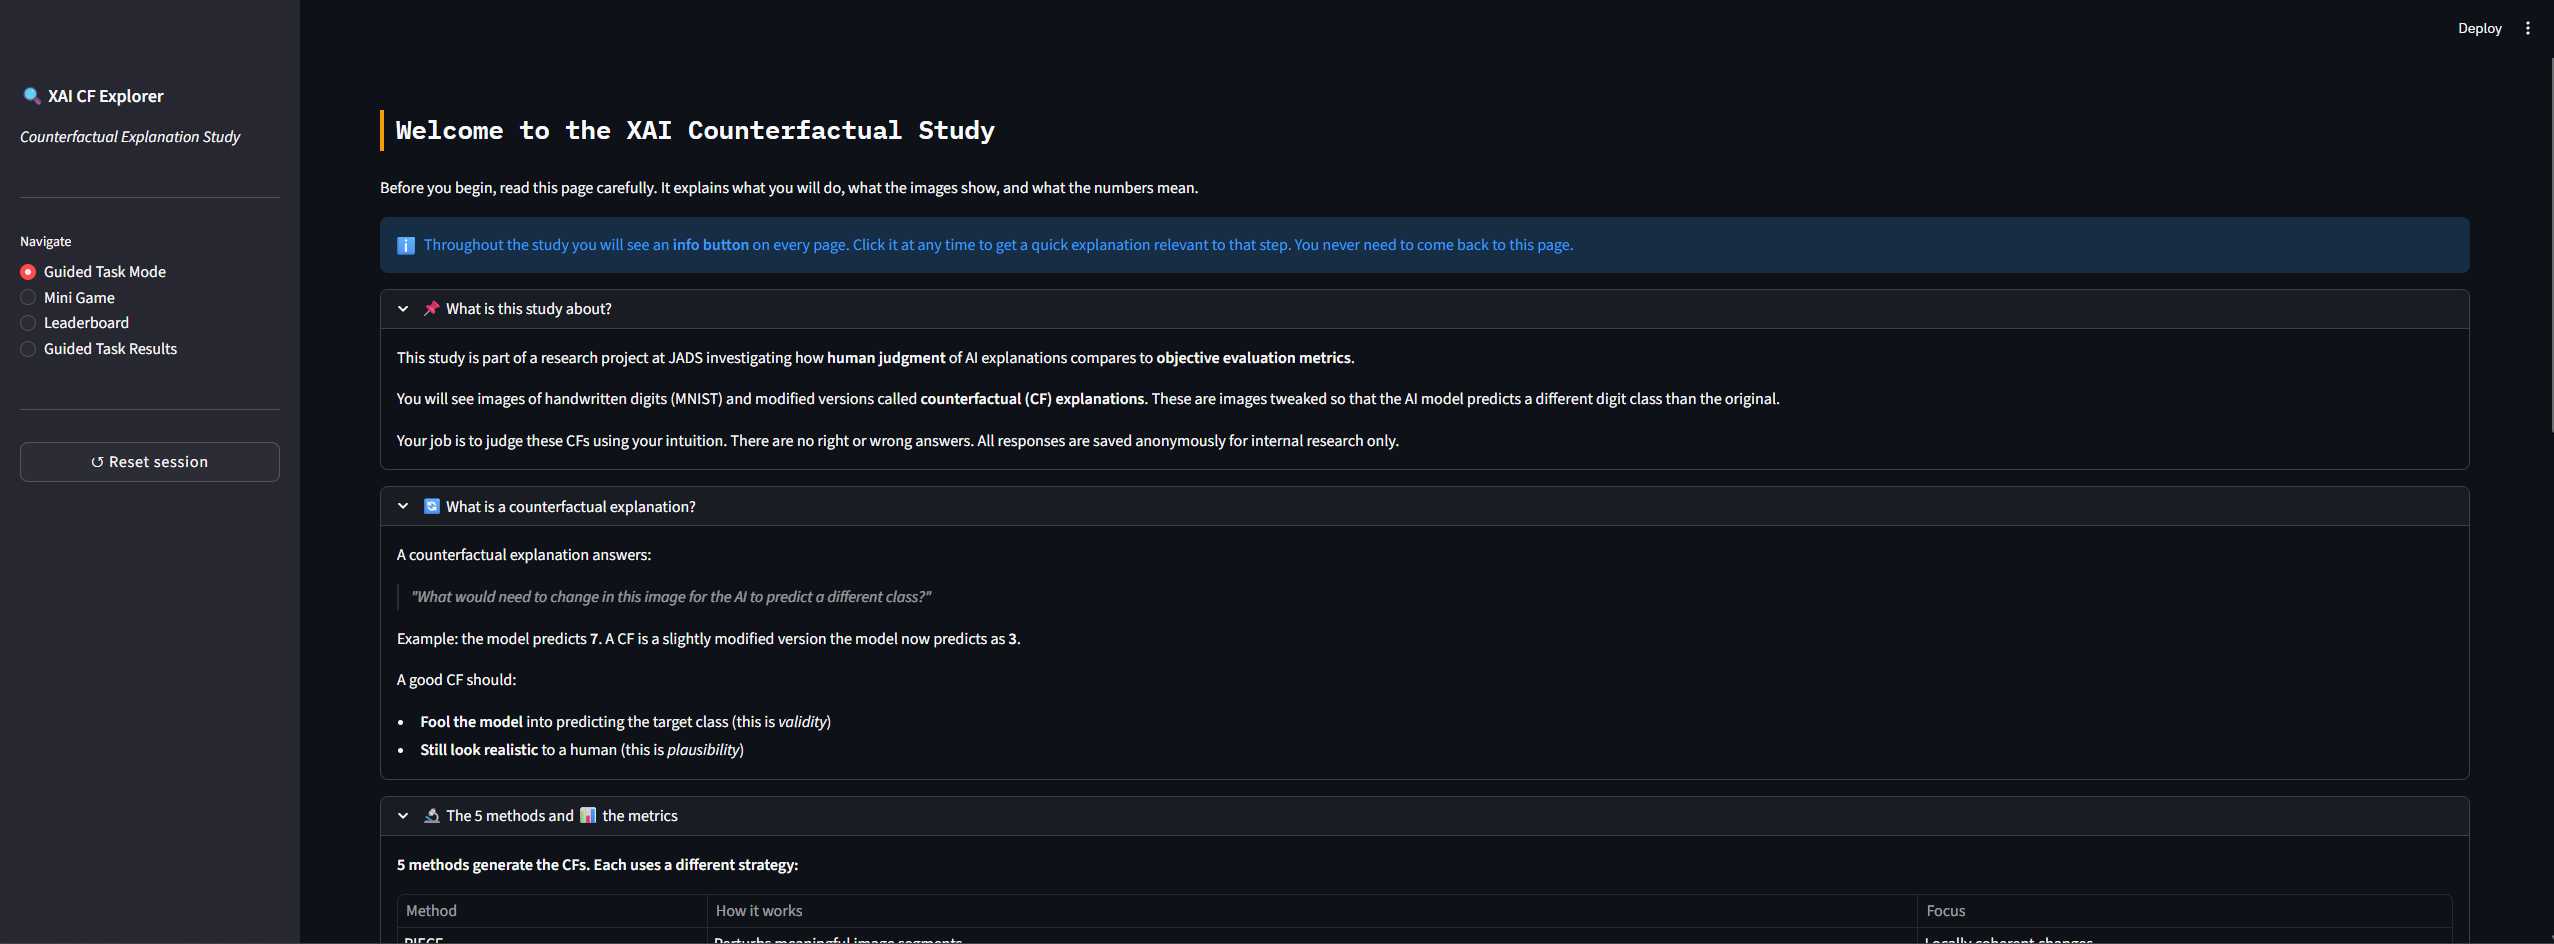
\includegraphics[keepaspectratio]{images/Final prototype/Home Screen Final Version.png}}

}

\caption{\label{fig-homescreen-1}HomeScreen 1}

\end{figure}%

\begin{figure}

\centering{

\pandocbounded{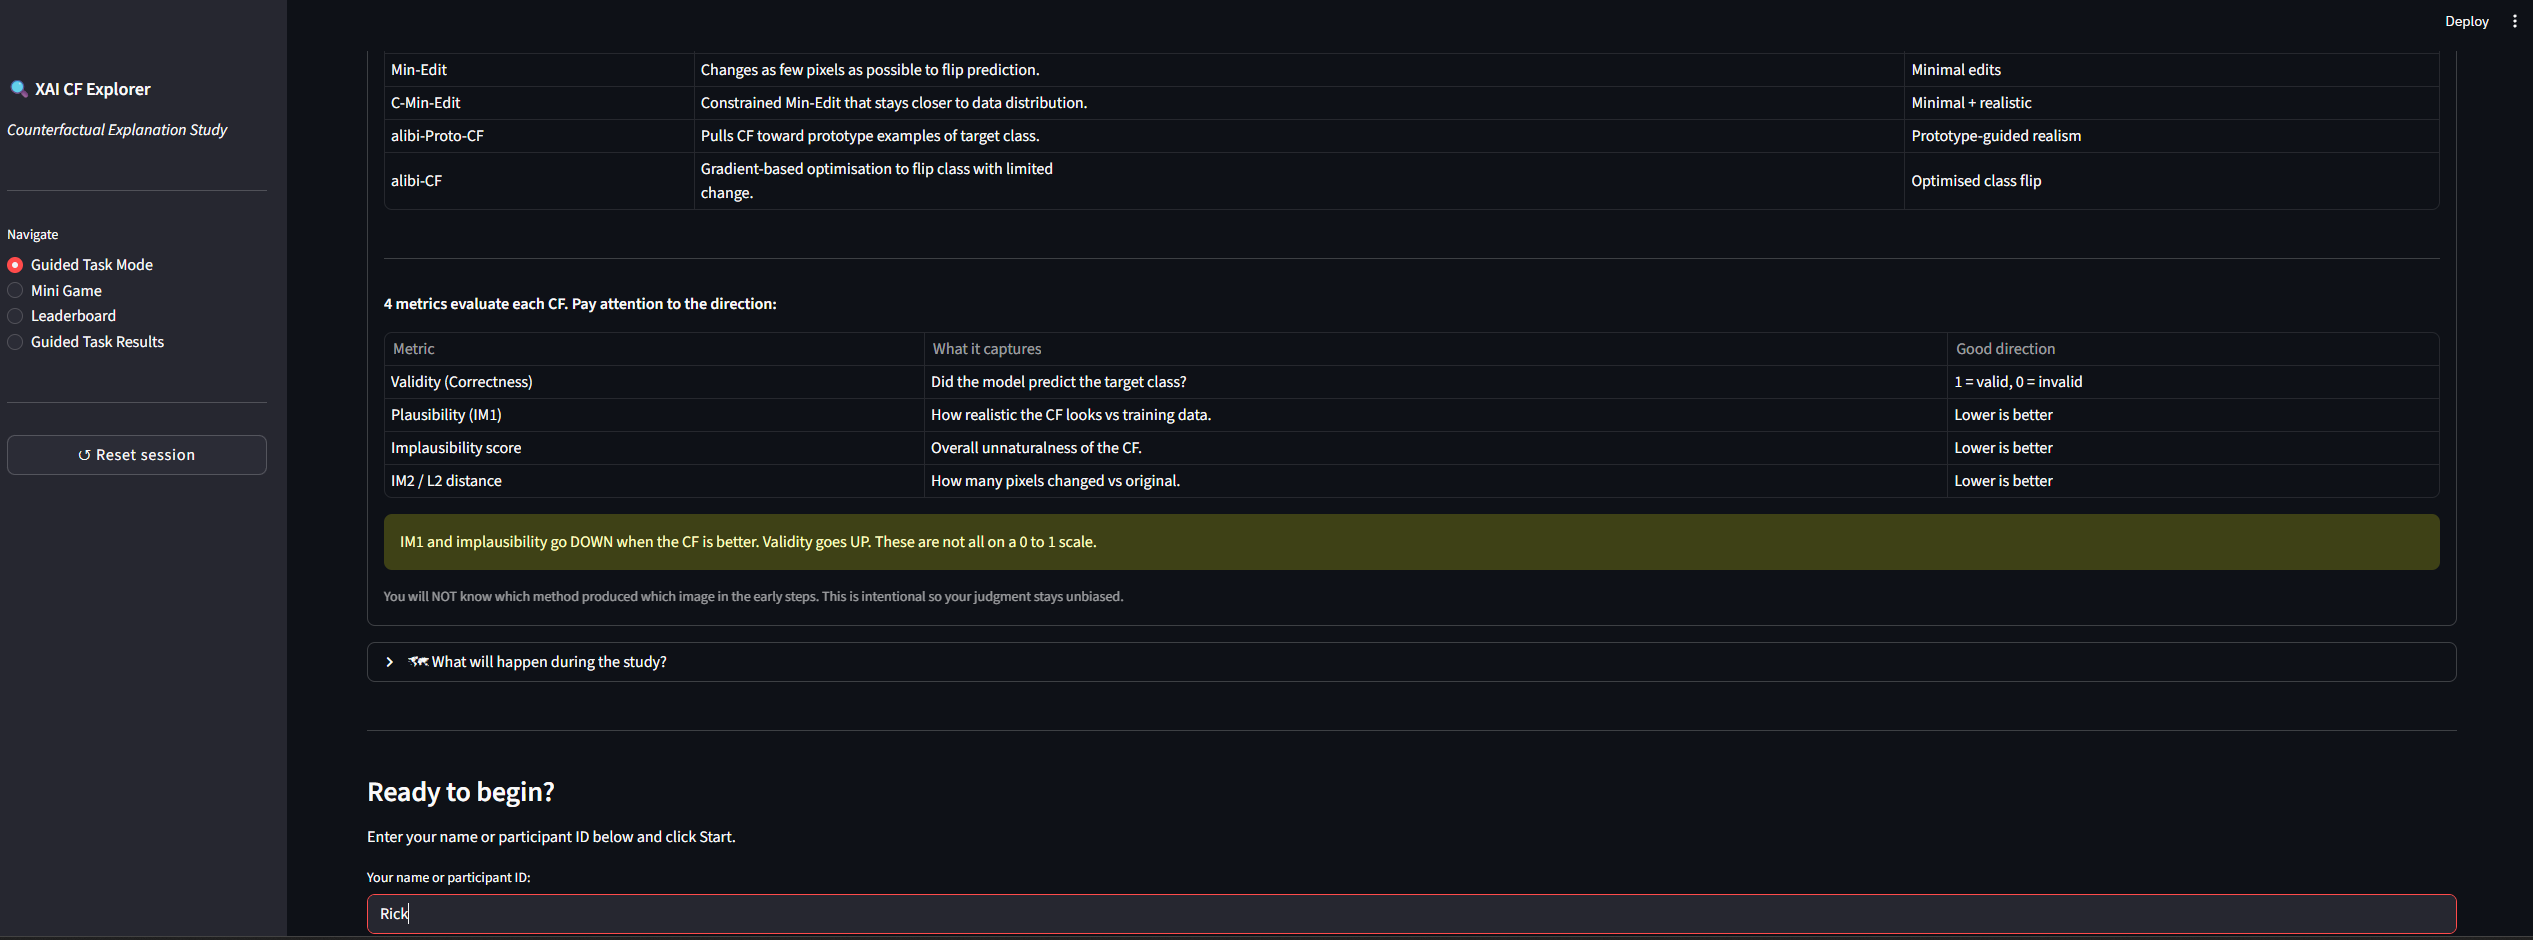
\includegraphics[keepaspectratio]{images/Final prototype/HomeScreen Final Version2.png}}

}

\caption{\label{fig-homescreen-2}Homescreen 2}

\end{figure}%

\begin{figure}

\centering{

\pandocbounded{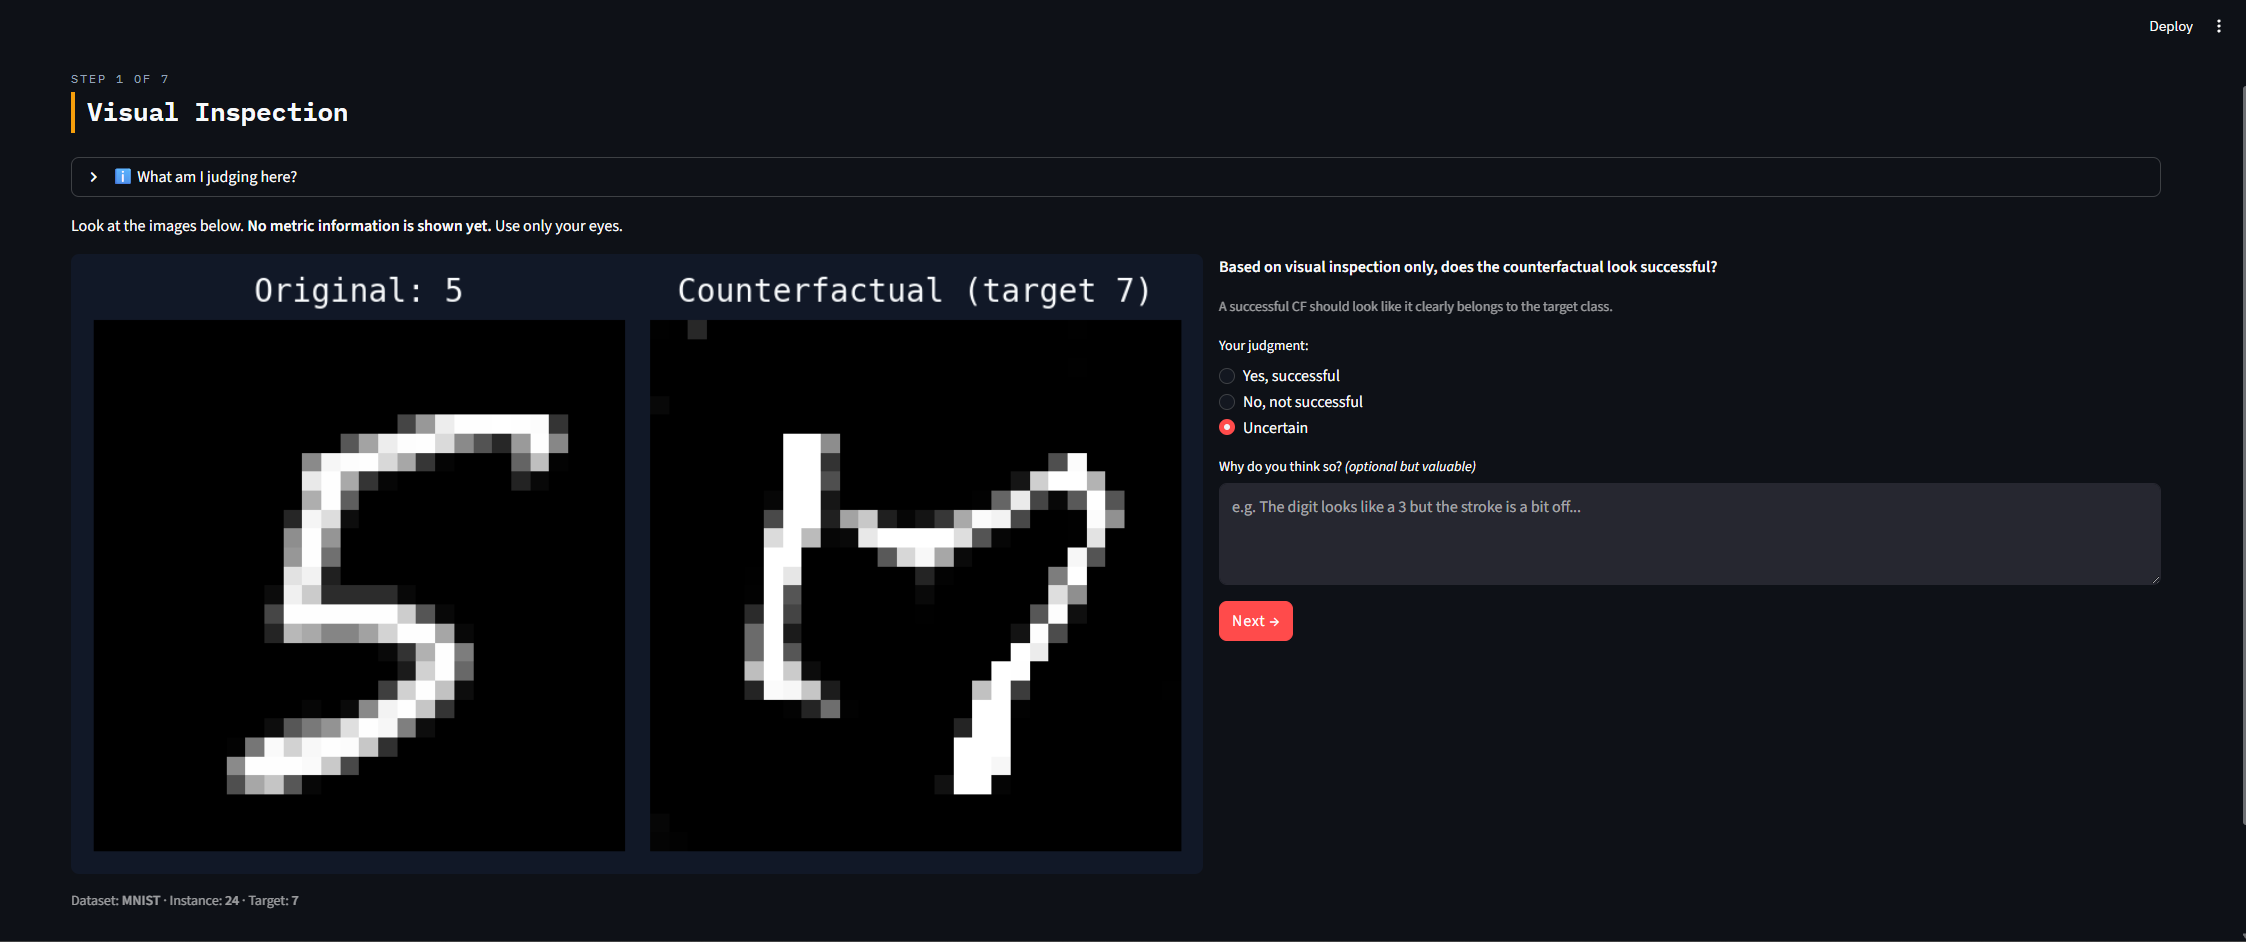
\includegraphics[keepaspectratio]{images/Final prototype/Visual Inspection Final Version.png}}

}

\caption{\label{fig-visual-inspec-fv}Visual Inspection FV}

\end{figure}%

\begin{figure}

\centering{

\pandocbounded{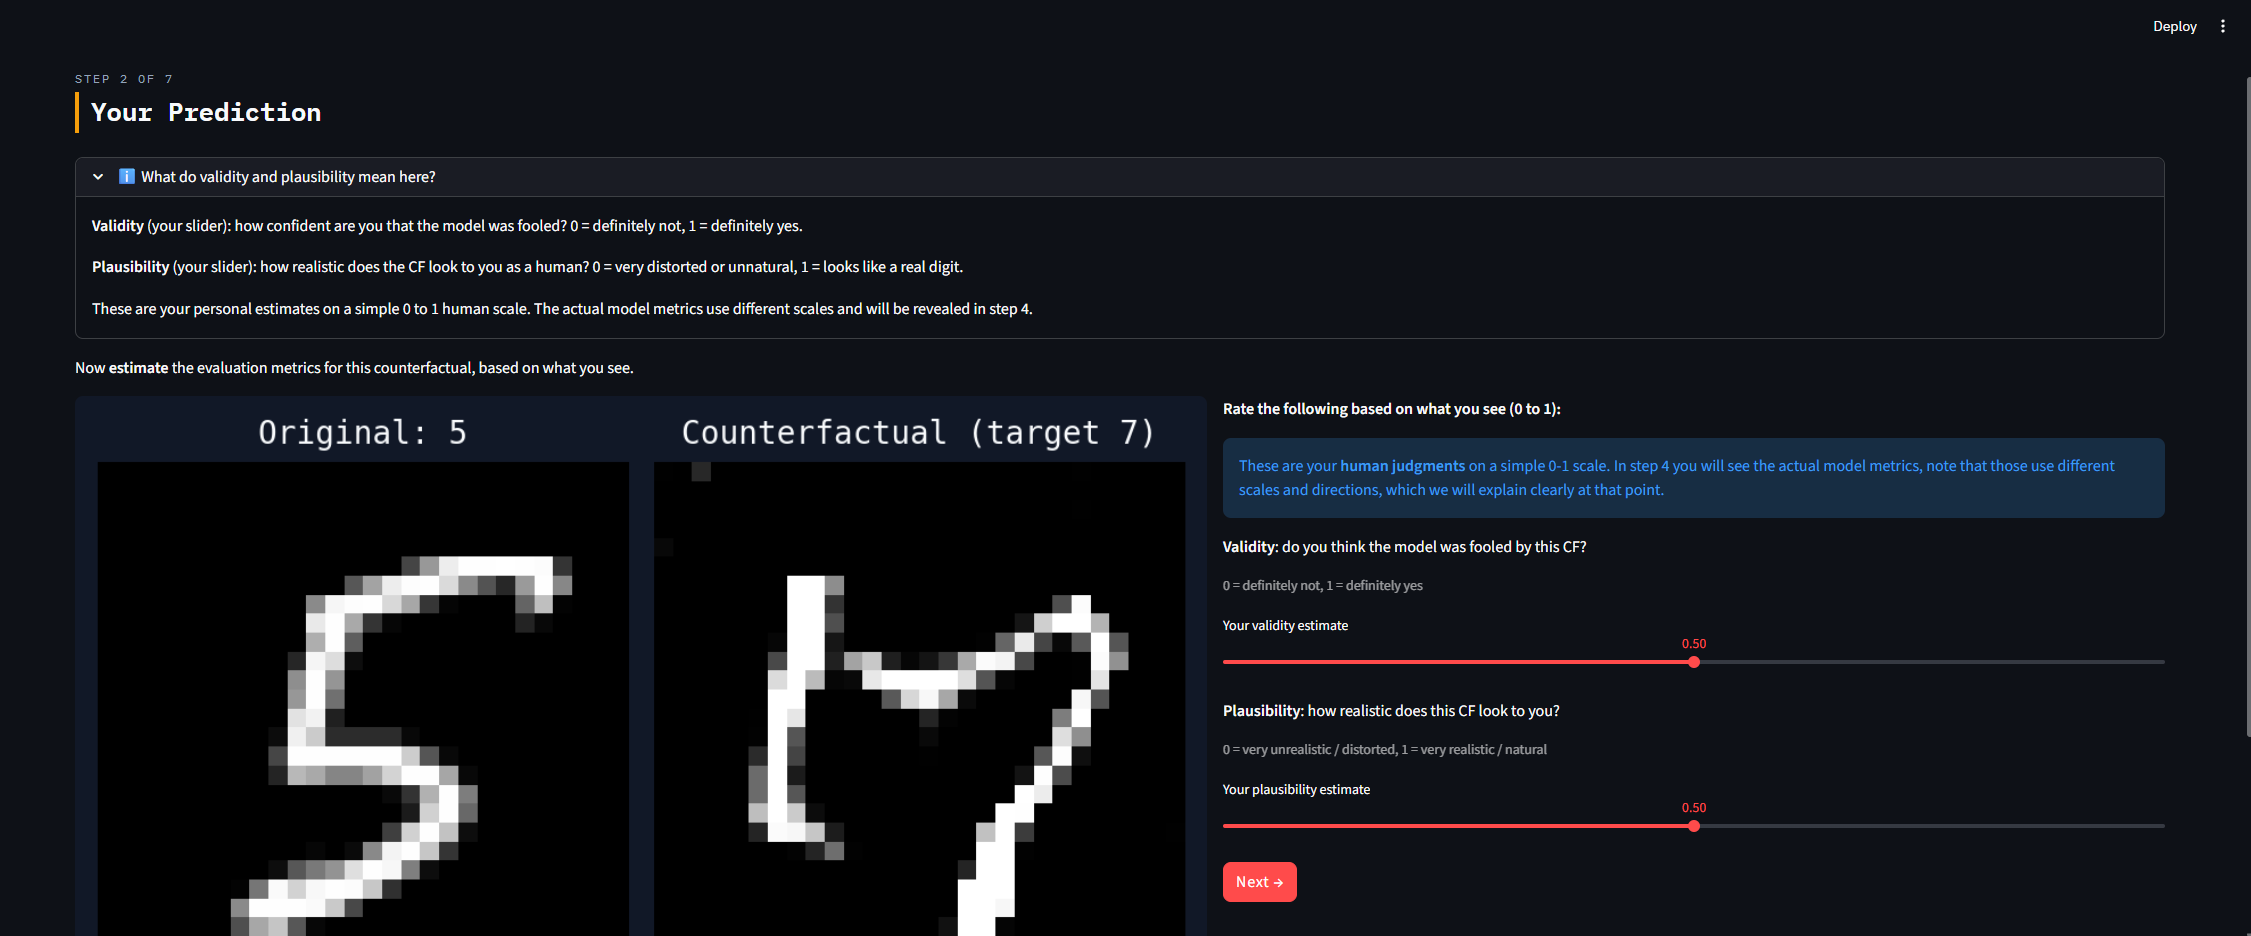
\includegraphics[keepaspectratio]{images/Final prototype/Your Prediction FV.png}}

}

\caption{\label{fig-user-pred-fv}User Prediction FV}

\end{figure}%

\begin{figure}

\centering{

\pandocbounded{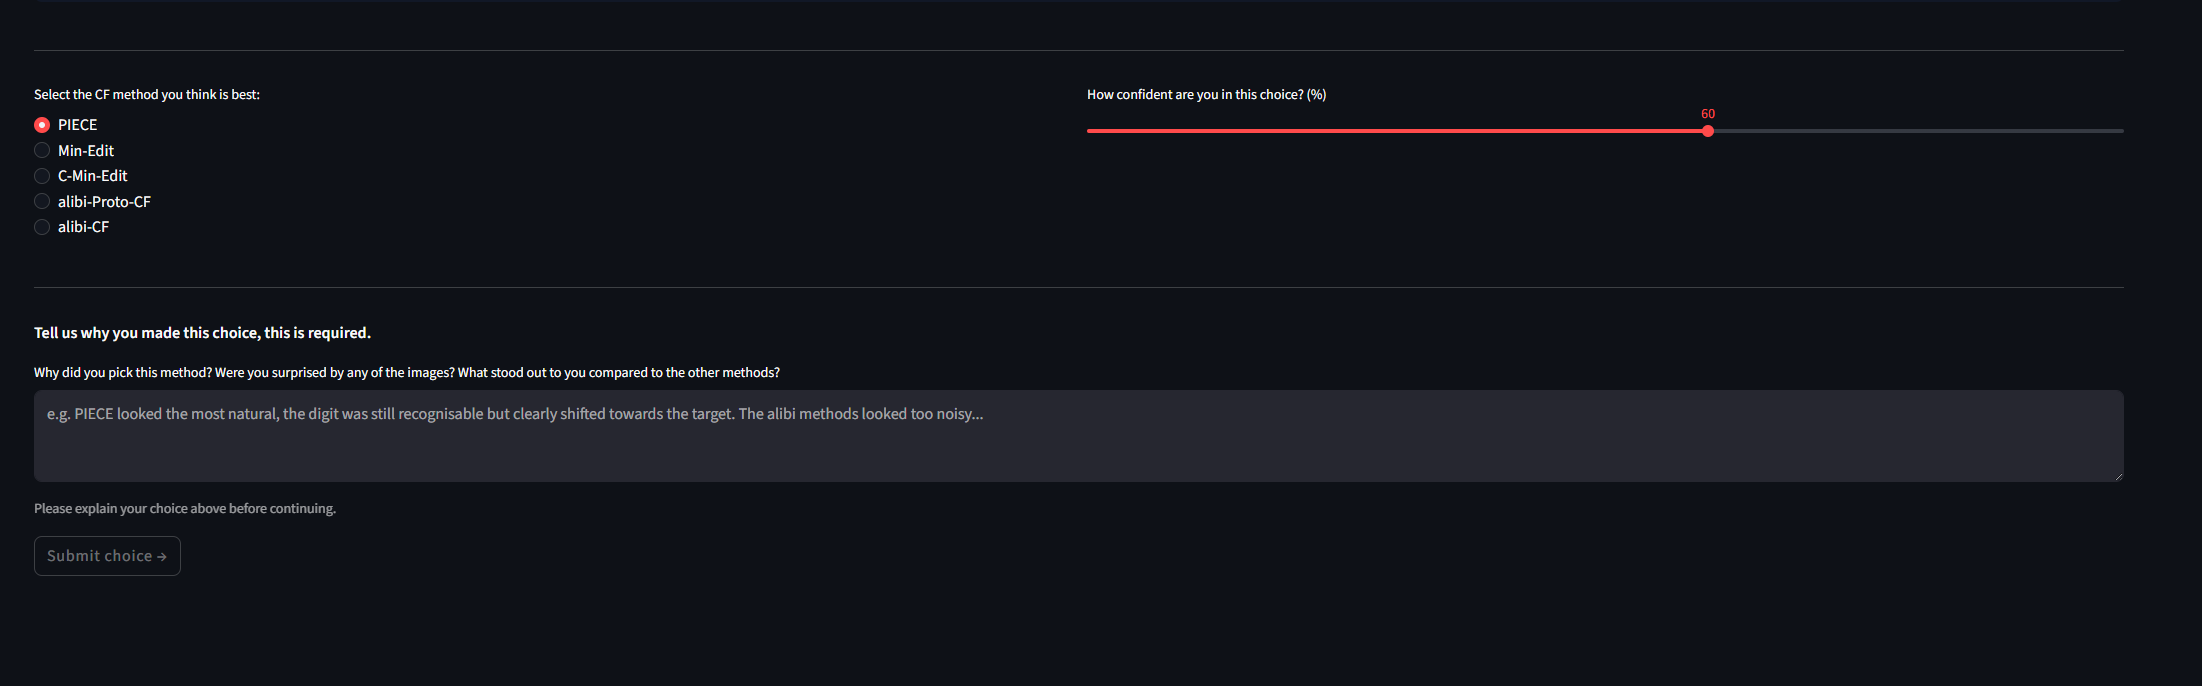
\includegraphics[keepaspectratio]{images/Final prototype/The Game FV2.png}}

}

\caption{\label{fig-game-fv}The Game}

\end{figure}%

\begin{figure}

\centering{

\pandocbounded{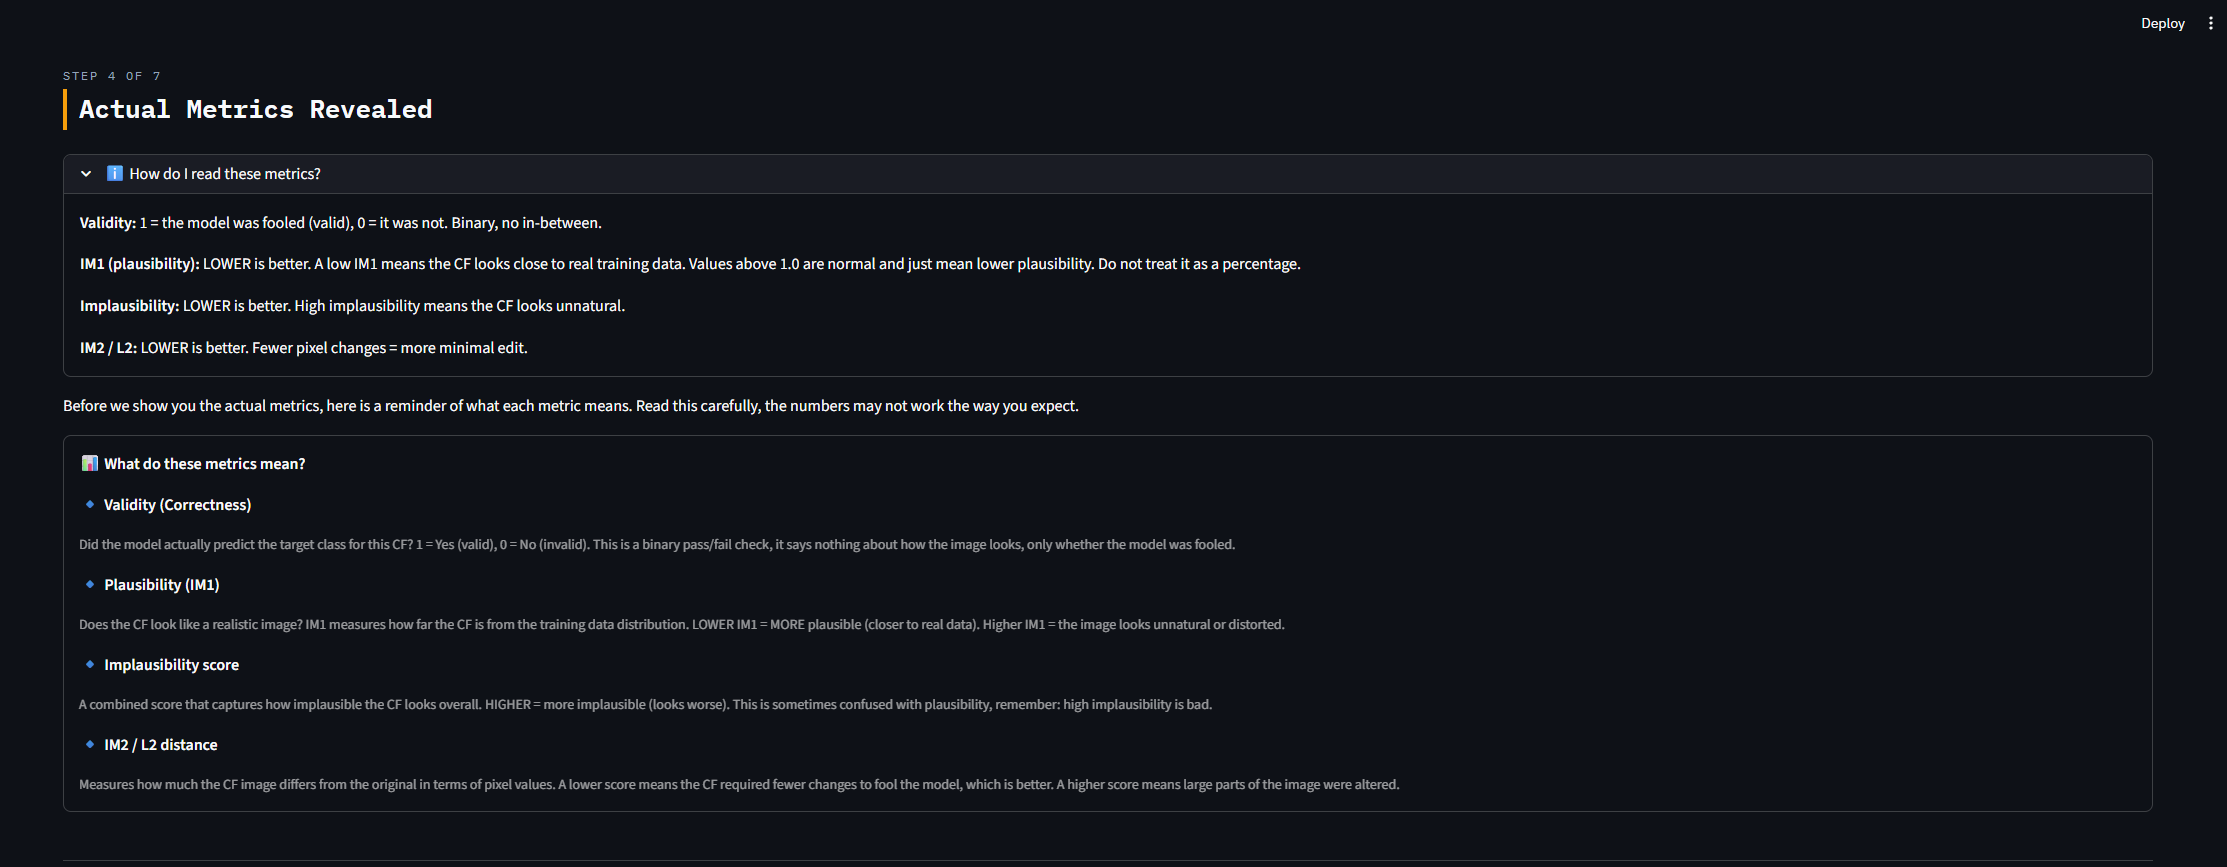
\includegraphics[keepaspectratio]{images/Final prototype/Actual Metrics FV.png}}

}

\caption{\label{fig-actual-1}Actual metrics 1}

\end{figure}%

\begin{figure}

\centering{

\pandocbounded{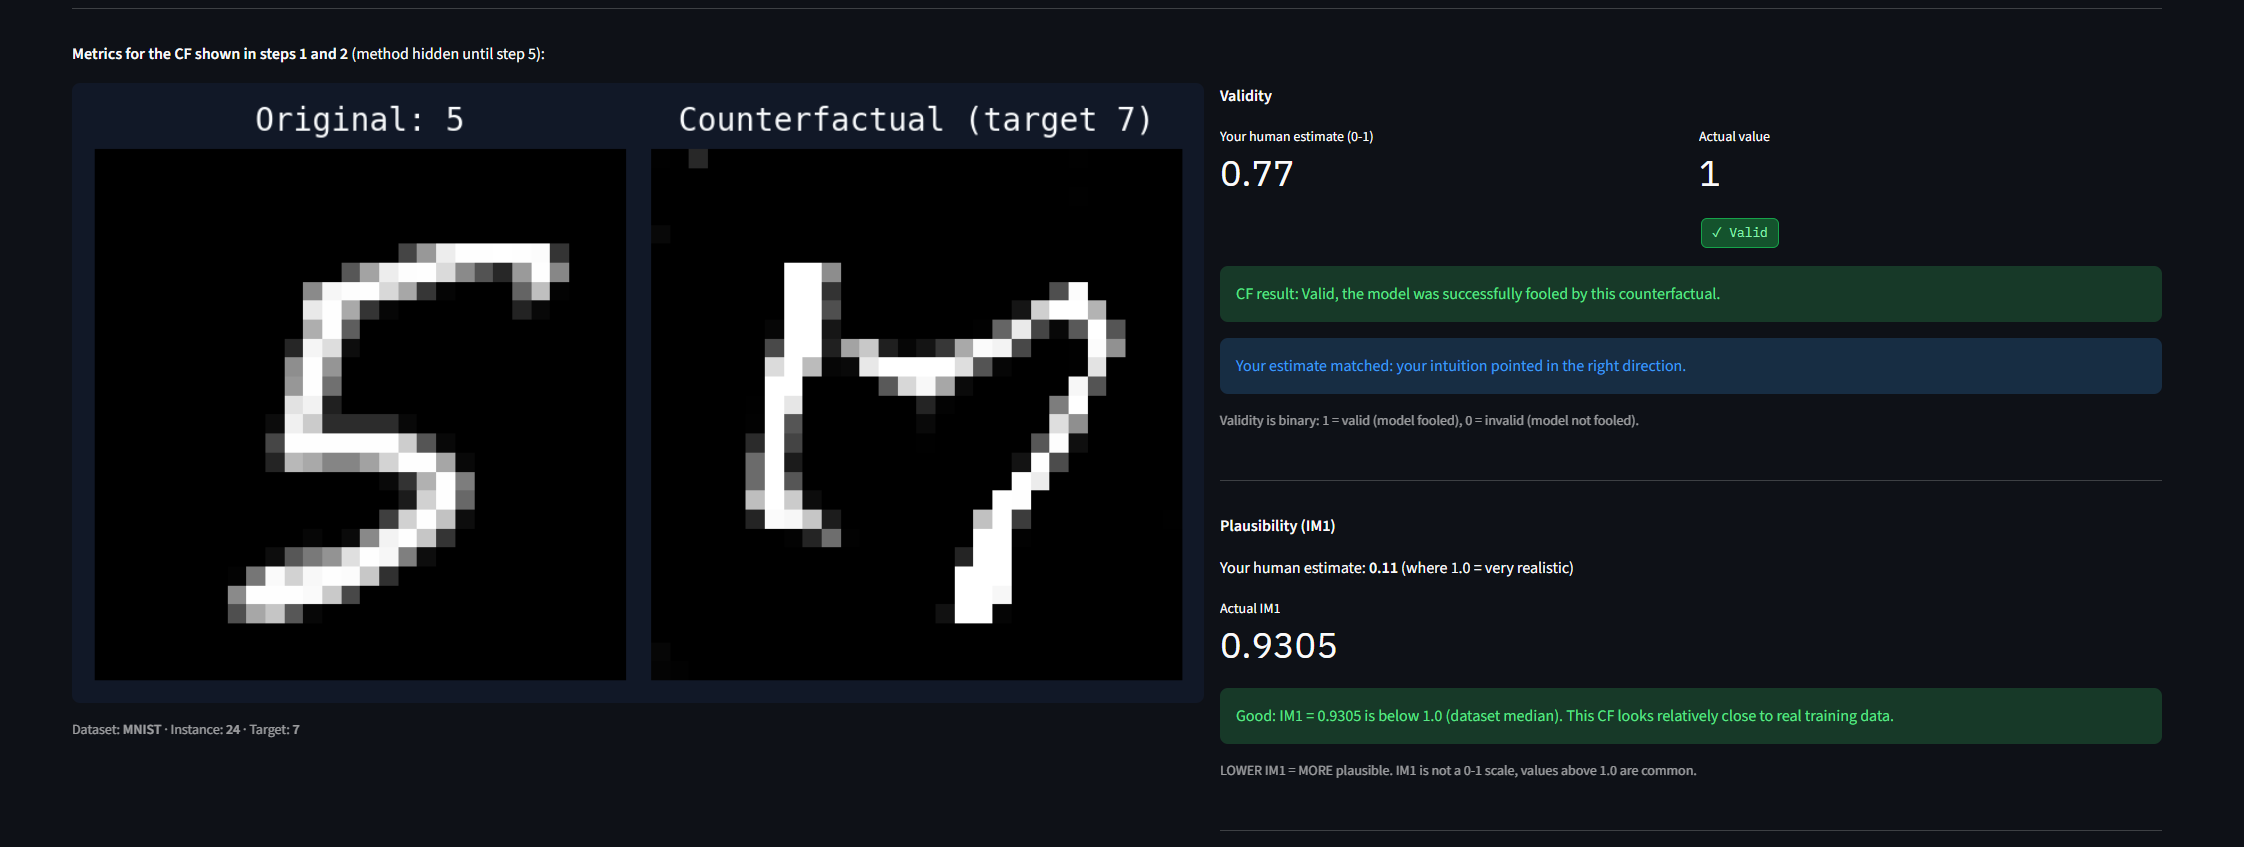
\includegraphics[keepaspectratio]{images/Final prototype/Actual Metrics 2.png}}

}

\caption{\label{fig-actual-2}Actual metric 2}

\end{figure}%

\pandocbounded{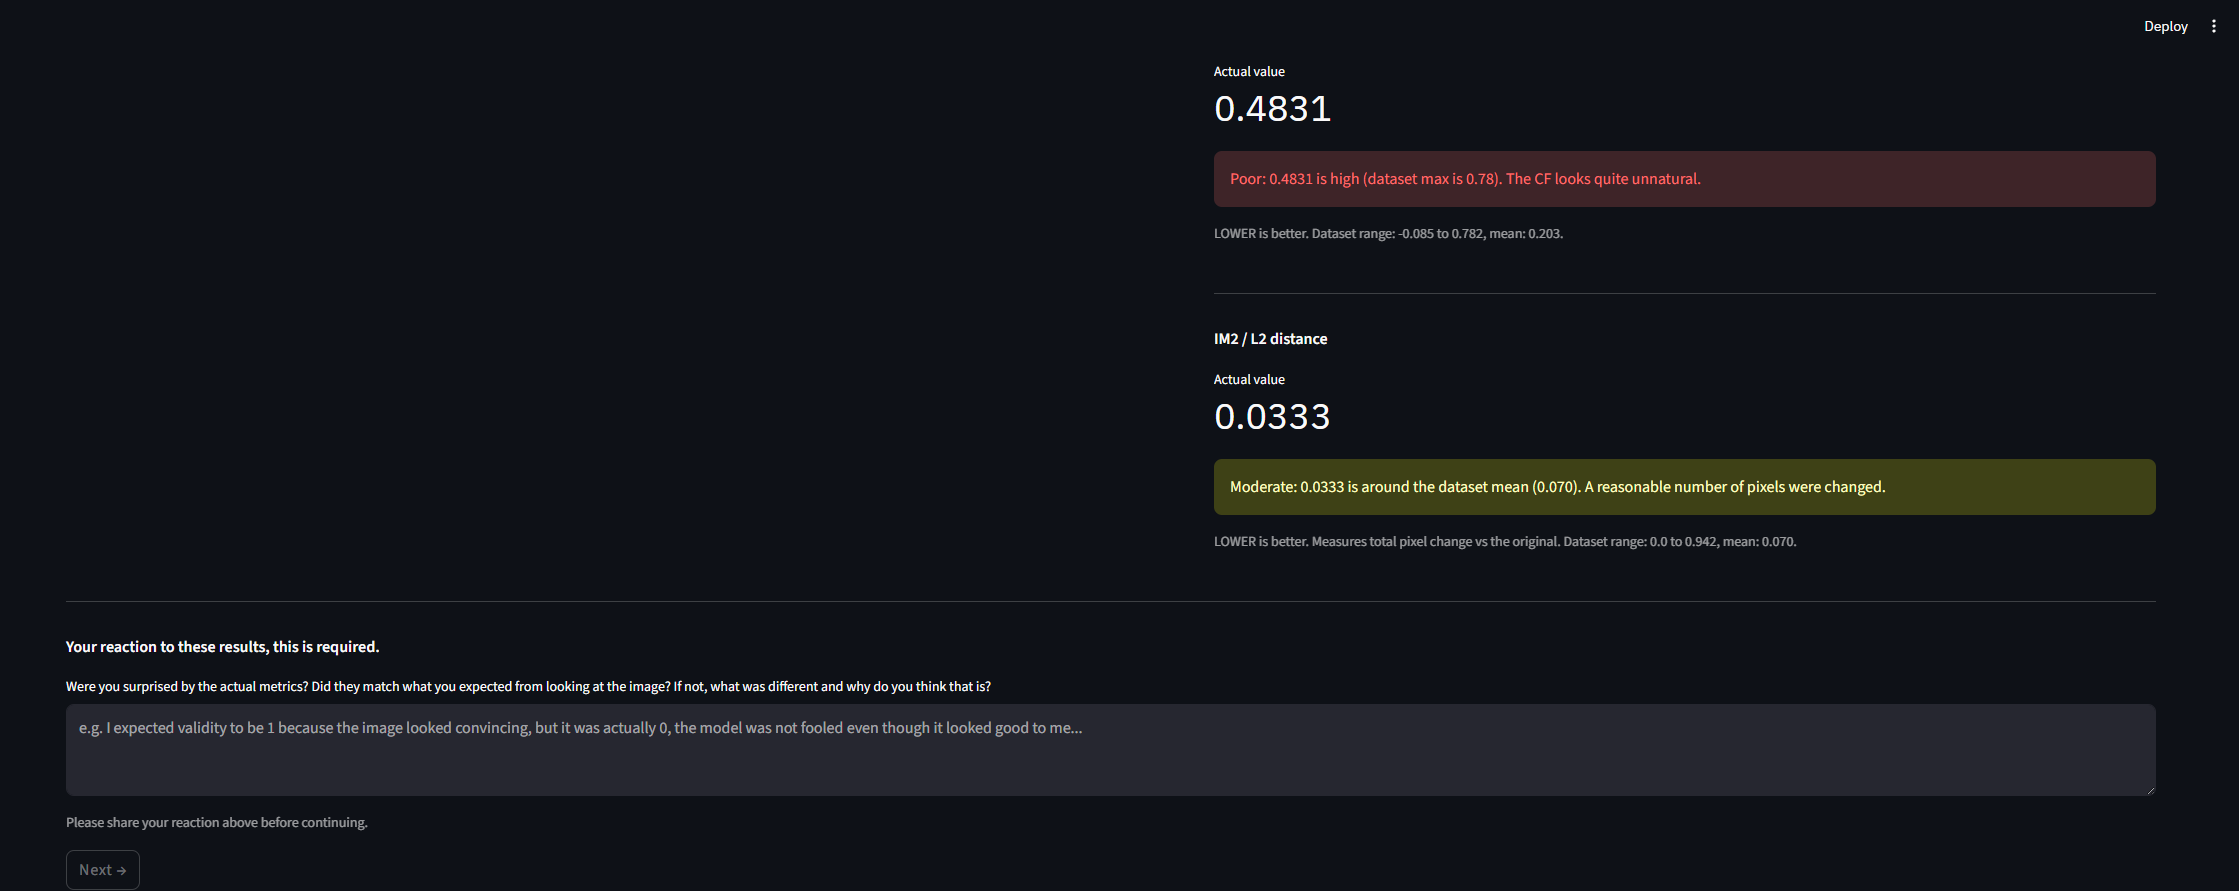
\includegraphics[keepaspectratio]{images/Final prototype/Actual Metrics FV 3.png}}\{\#fig-actual
metric 3\}

\begin{figure}[H]

{\centering \pandocbounded{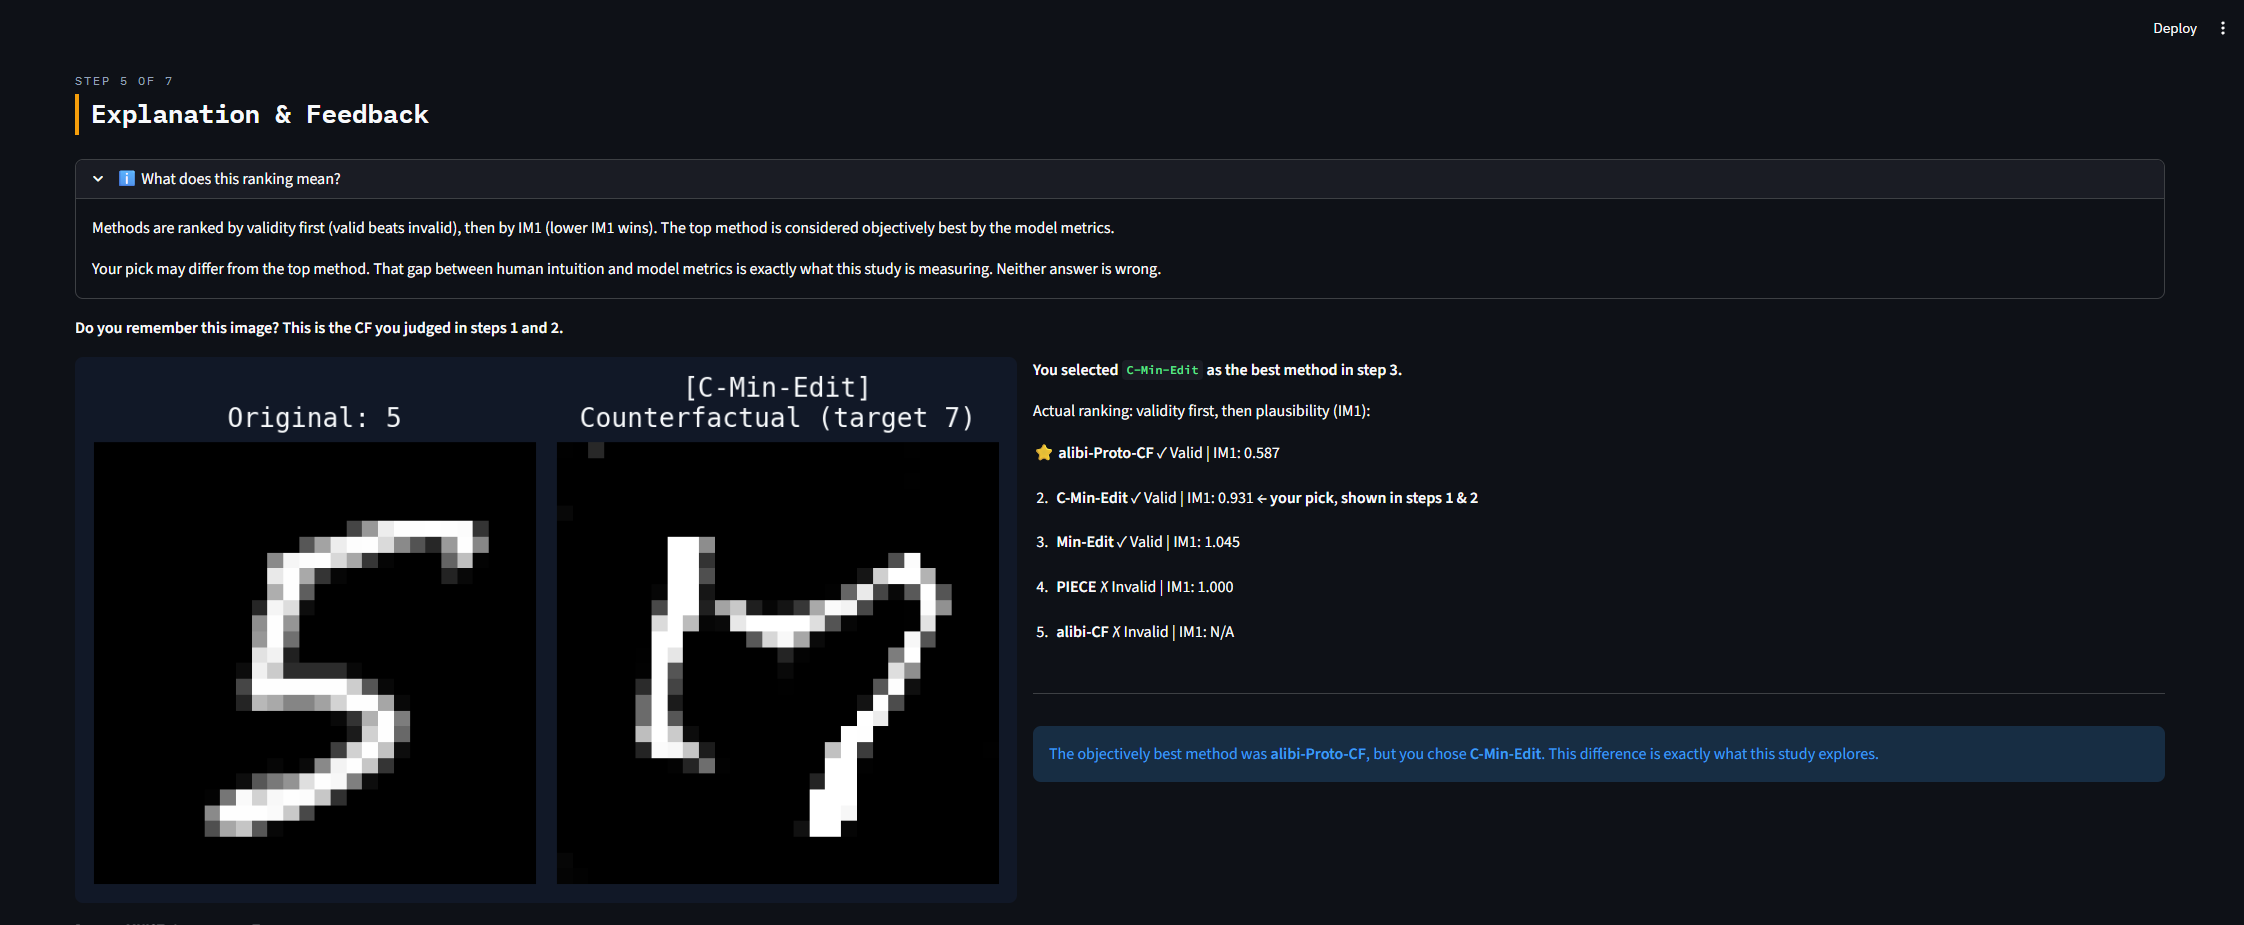
\includegraphics[keepaspectratio]{images/Final prototype/Explanation & Feedback 1.png}}

}

\caption{Explanation \& Feedback FV 1}

\end{figure}%

\begin{figure}

\centering{

\pandocbounded{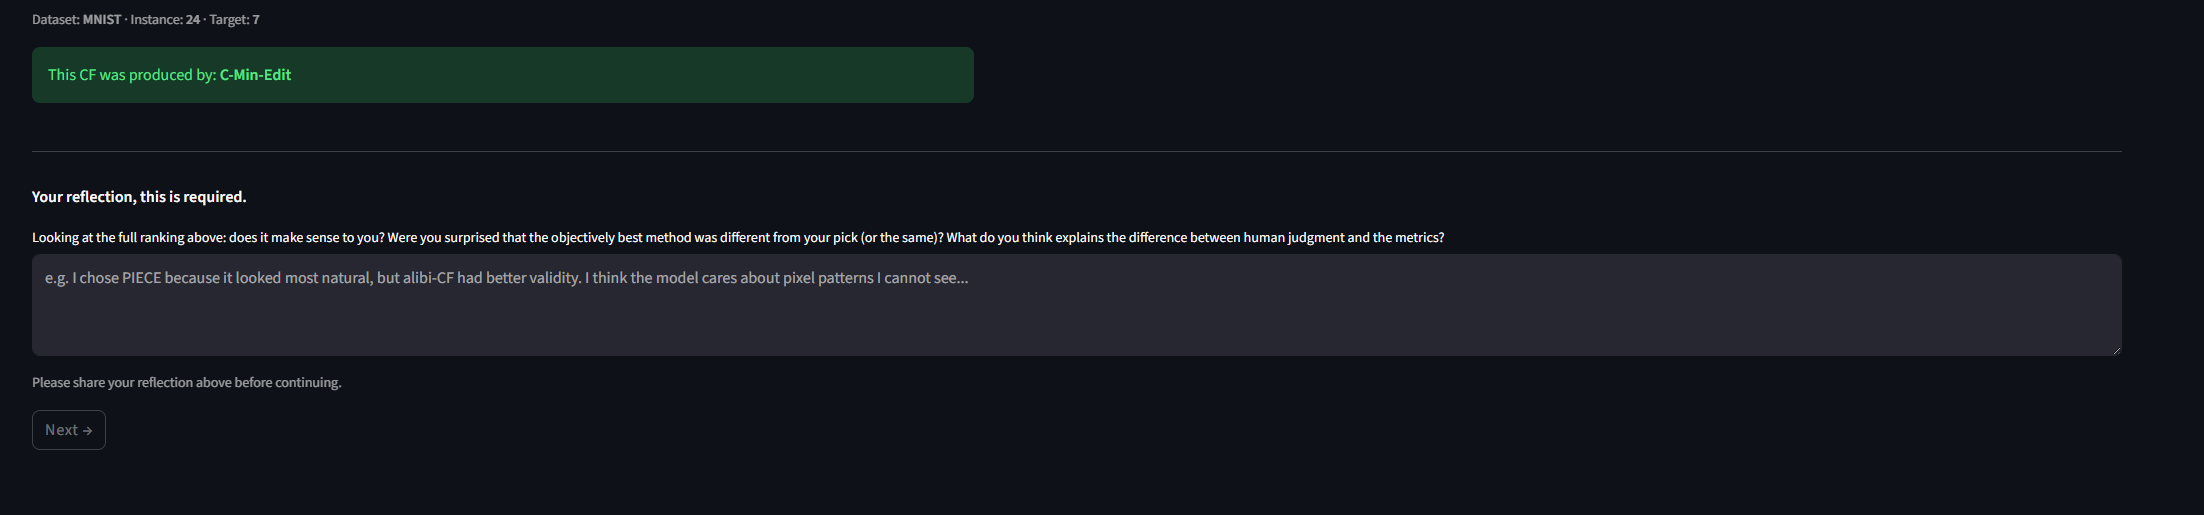
\includegraphics[keepaspectratio]{images/Final prototype/Explanation & feedback 2.png}}

}

\caption{\label{fig-expla-2}Explanation \& Feedback 2}

\end{figure}%

\begin{figure}[H]

{\centering \pandocbounded{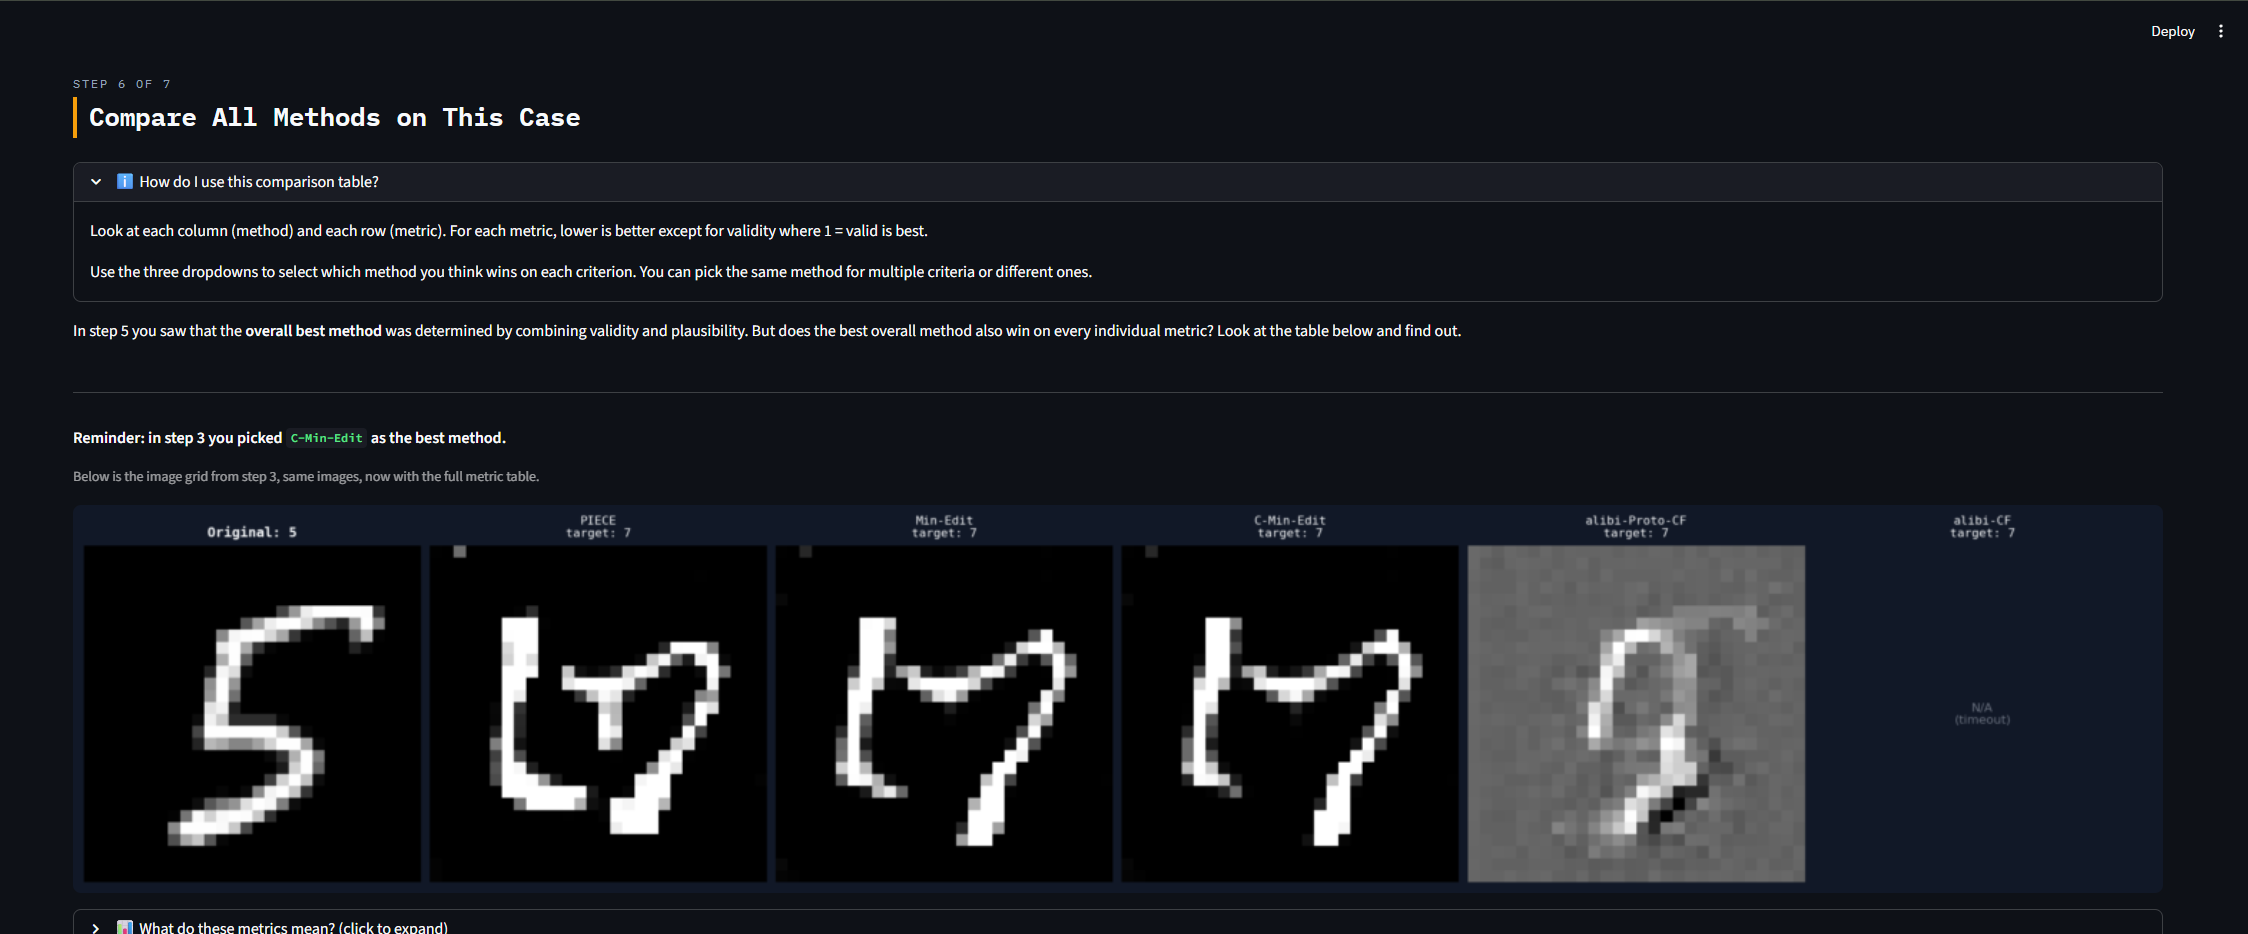
\includegraphics[keepaspectratio]{images/Final prototype/Compare all methods 1.png}}

}

\caption{Compare methods FV 1}

\end{figure}%%
\begin{figure}[H]

{\centering \pandocbounded{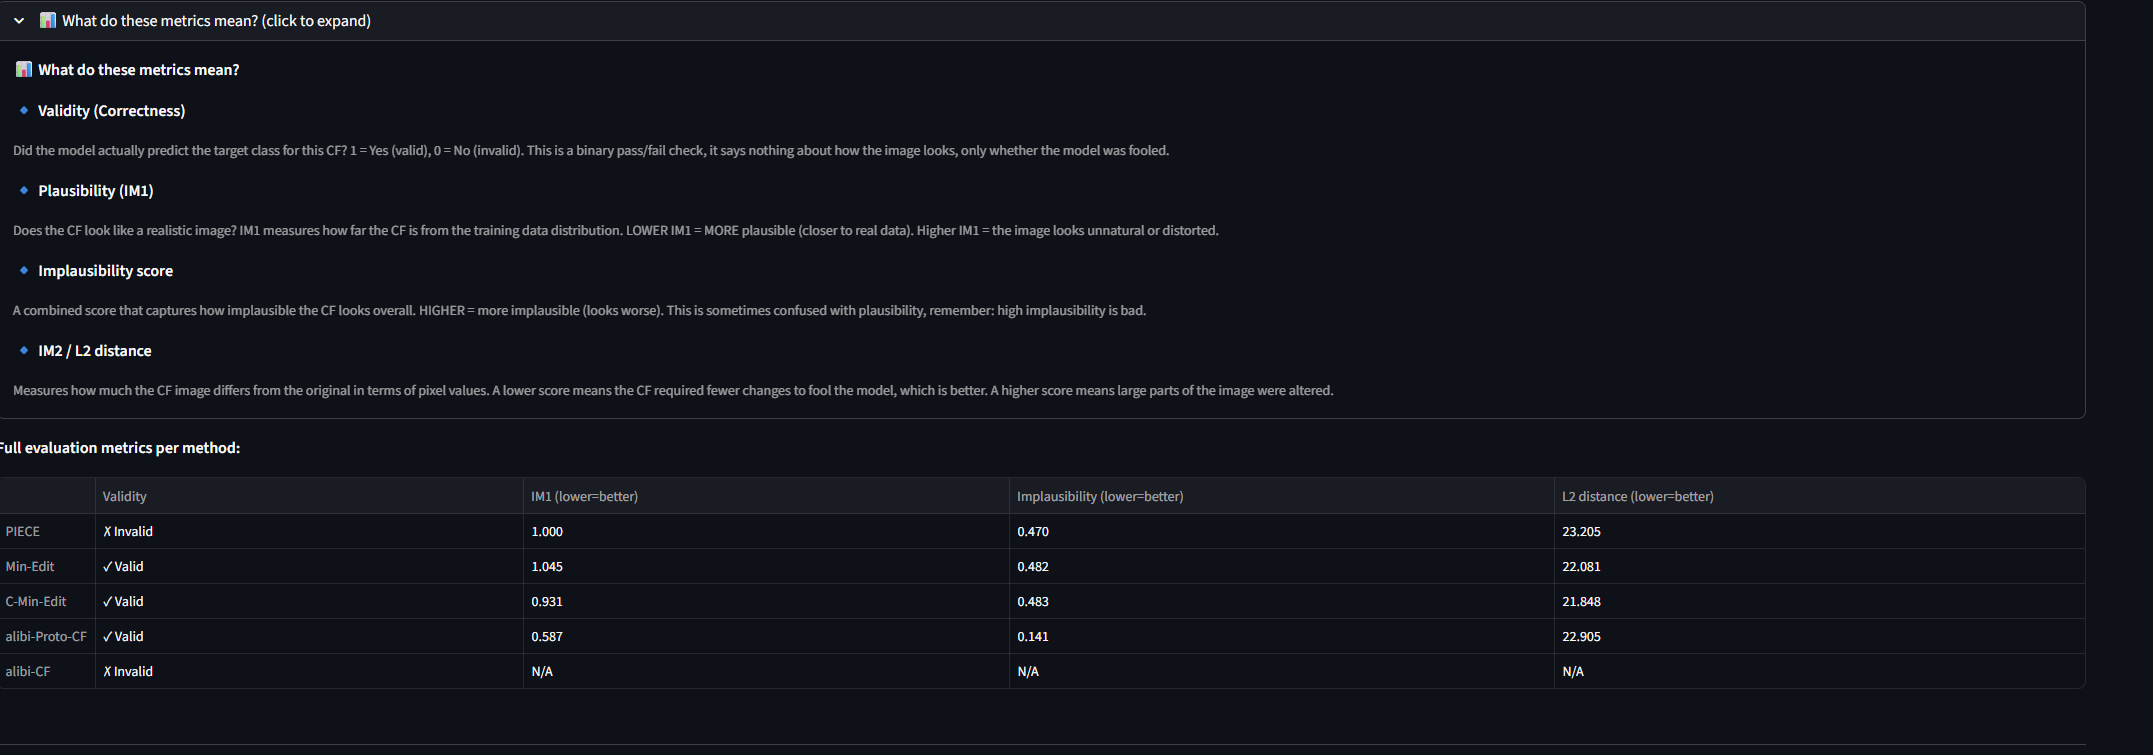
\includegraphics[keepaspectratio]{images/Final prototype/Compare all methods 2.png}}

}

\caption{Compare methods 2 FV}

\end{figure}%%
\begin{figure}[H]

{\centering \pandocbounded{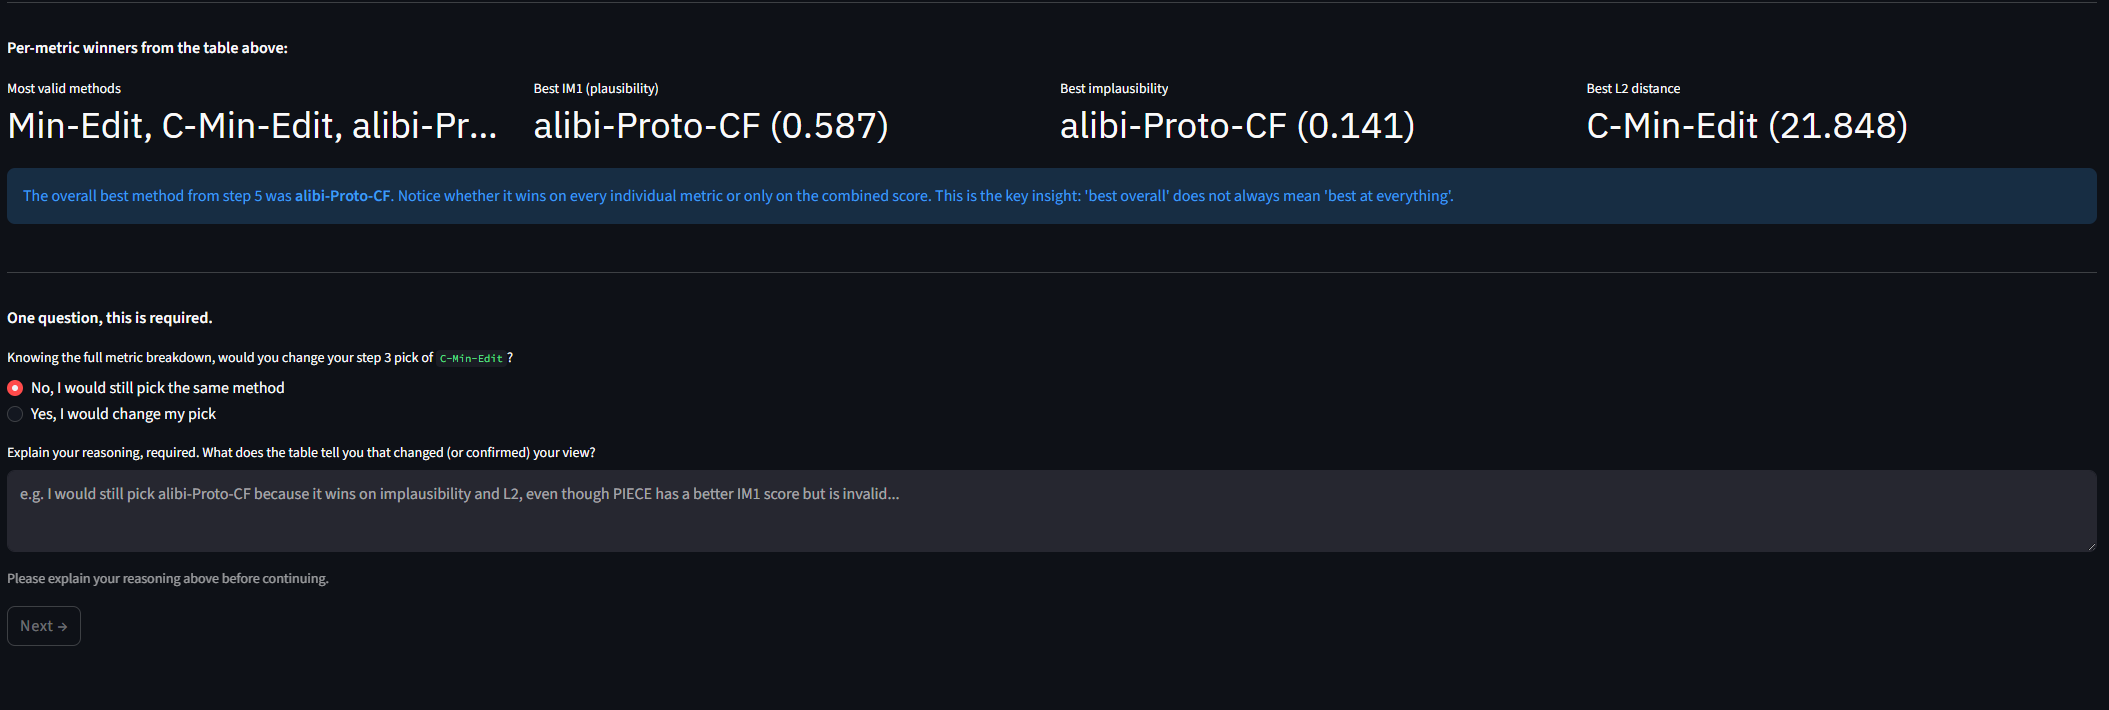
\includegraphics[keepaspectratio]{images/Final prototype/Compare all methods 3.png}}

}

\caption{Compare methods FV 3}

\end{figure}%%
\begin{figure}[H]

{\centering \pandocbounded{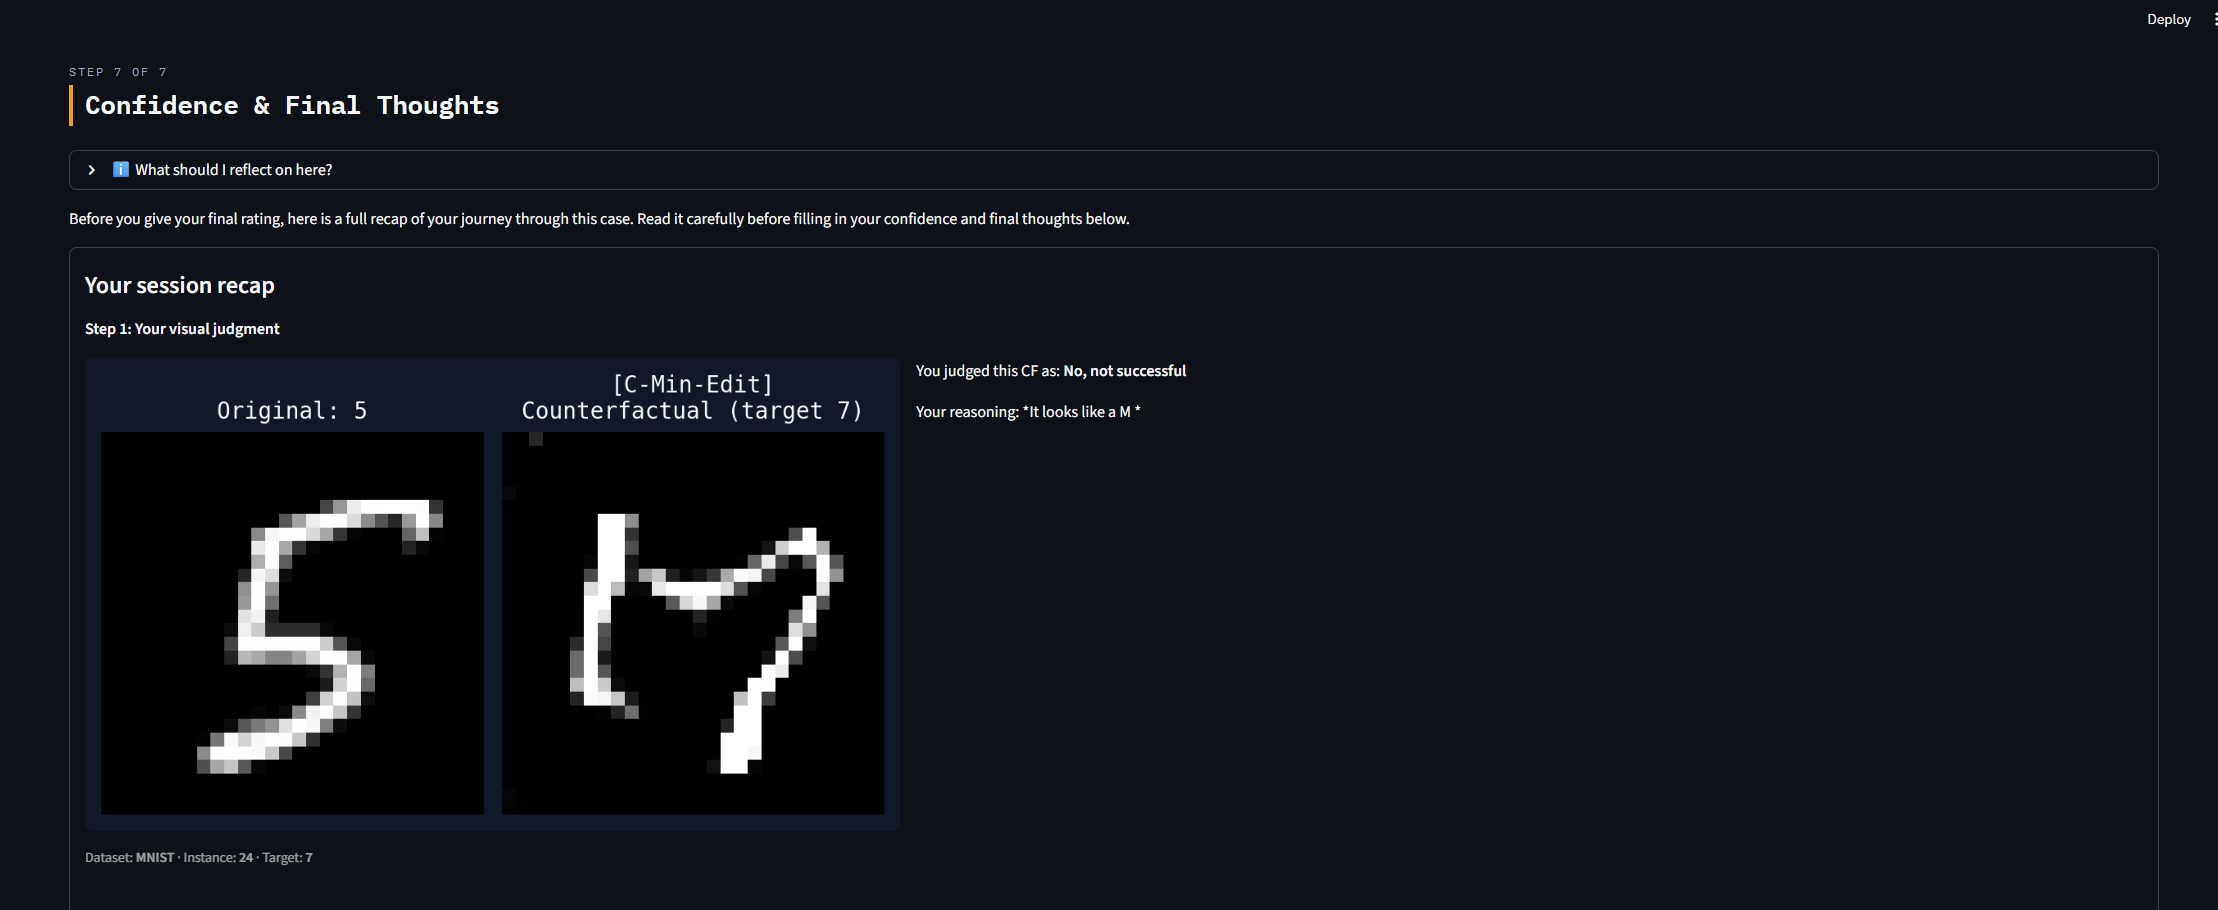
\includegraphics[keepaspectratio]{images/Confidence & Final Thoughts.png}}

}

\caption{Final Thought \& Confidence FV 1}

\end{figure}%%
\begin{figure}[H]

{\centering \pandocbounded{\includegraphics[keepaspectratio]{images/Final prototype/Confidence & final thoughts 2.png}}

}

\caption{Final Thought \& Confidence 2}

\end{figure}%%
\begin{figure}[H]

{\centering \pandocbounded{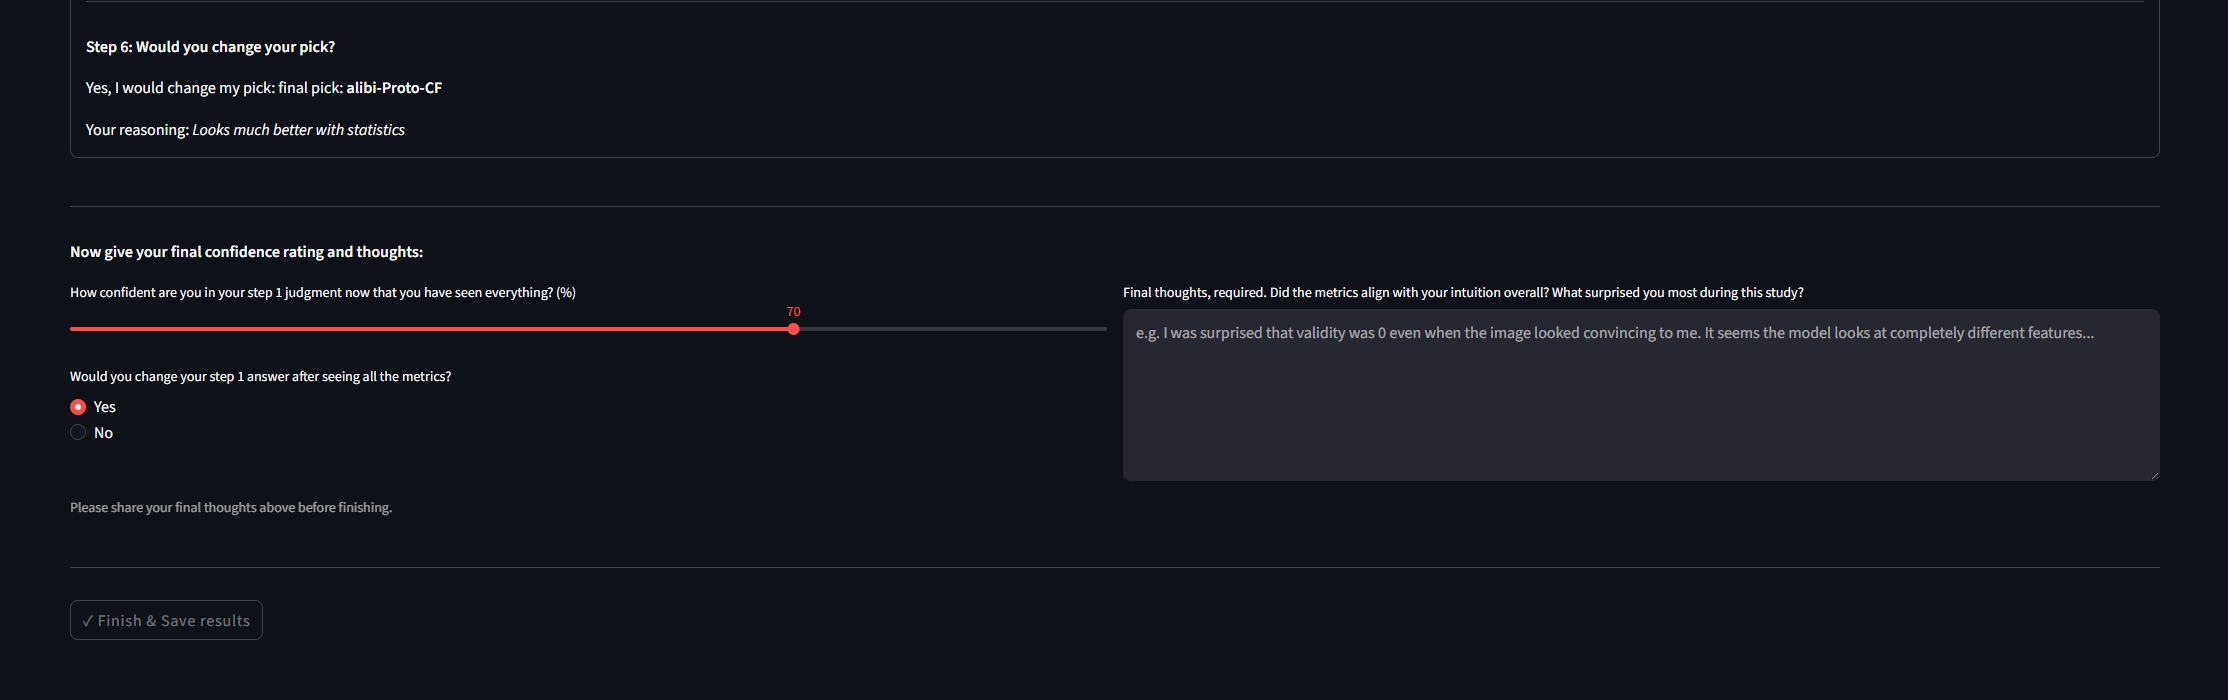
\includegraphics[keepaspectratio]{images/confidence 3.png}}

}

\caption{Confidence 3}

\end{figure}%

\section{Appendix Archive
Prototype}\label{sec-appendix-archive-prototype}

\begin{figure}

\centering{


\includegraphics[width=17.64583in,height=\textheight,keepaspectratio]{images/Filling_in_name.png}

}

\caption{\label{fig-home}Homescreen}

\end{figure}%

\begin{figure}

\centering{

\pandocbounded{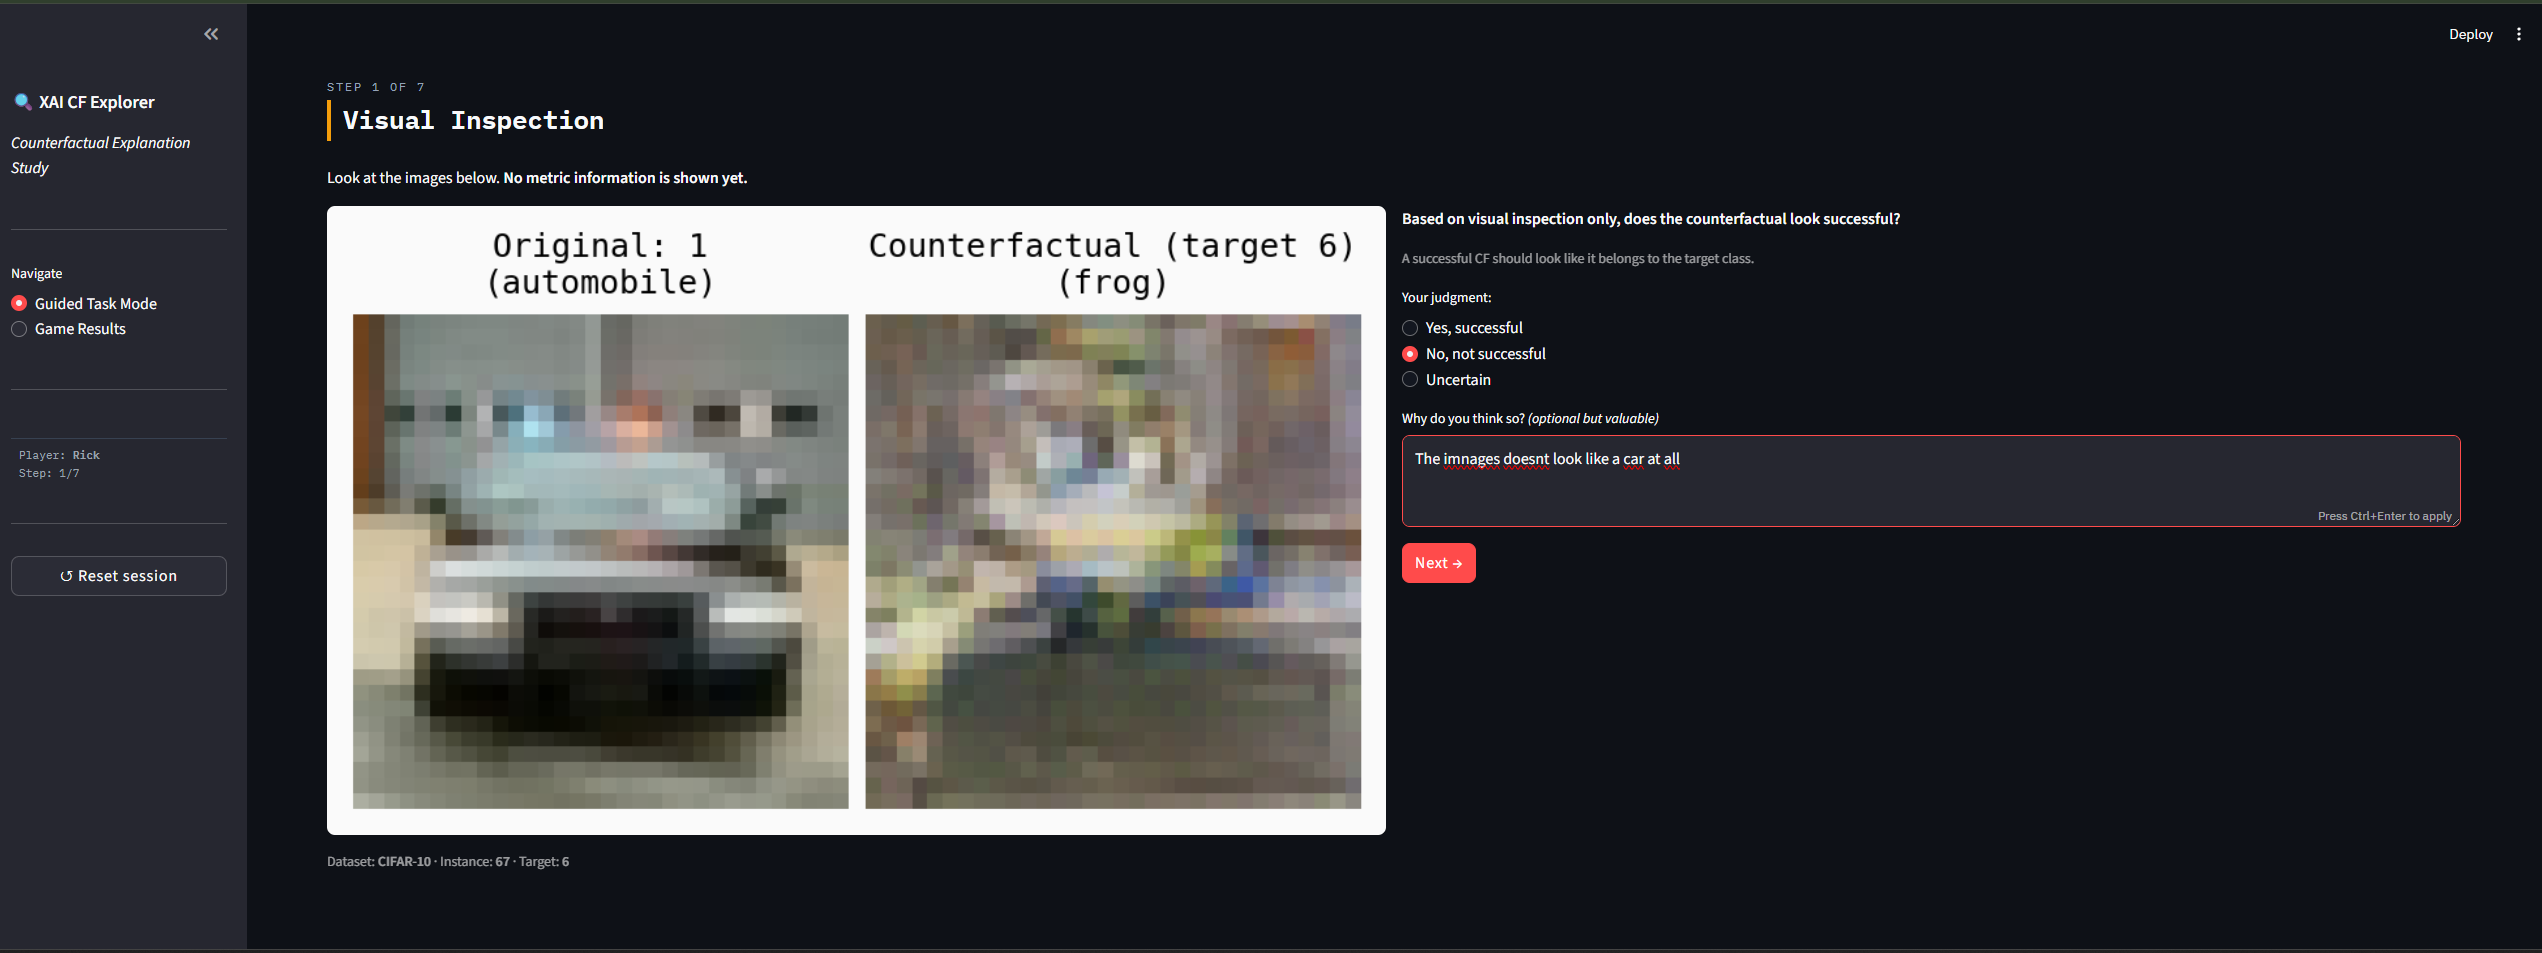
\includegraphics[keepaspectratio]{images/Visual-Inspection.png}}

}

\caption{\label{fig-visual}Visual Inspection}

\end{figure}%

\begin{figure}

\centering{

\pandocbounded{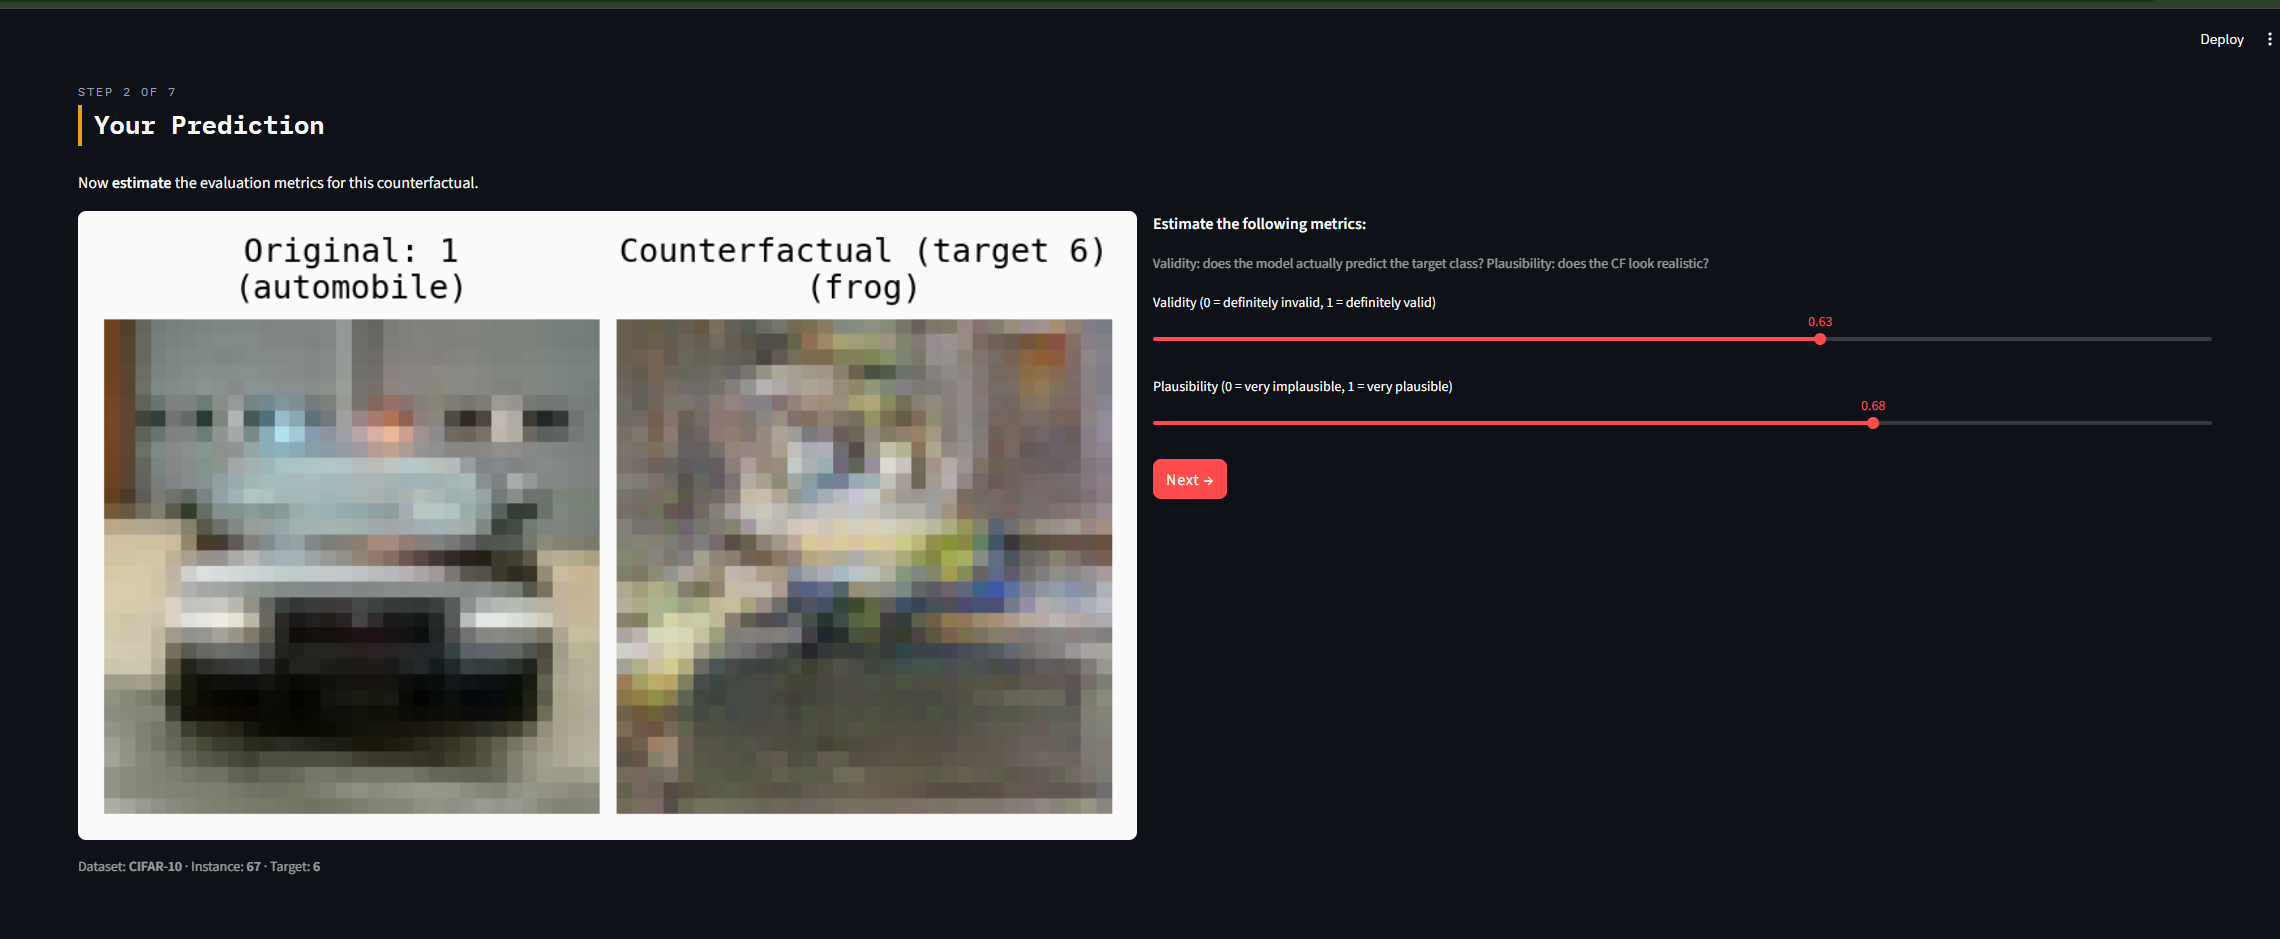
\includegraphics[keepaspectratio]{images/Your prediciton (3).png}}

}

\caption{\label{fig-prediction-users}User Prediction}

\end{figure}%

\begin{figure}

\centering{

\pandocbounded{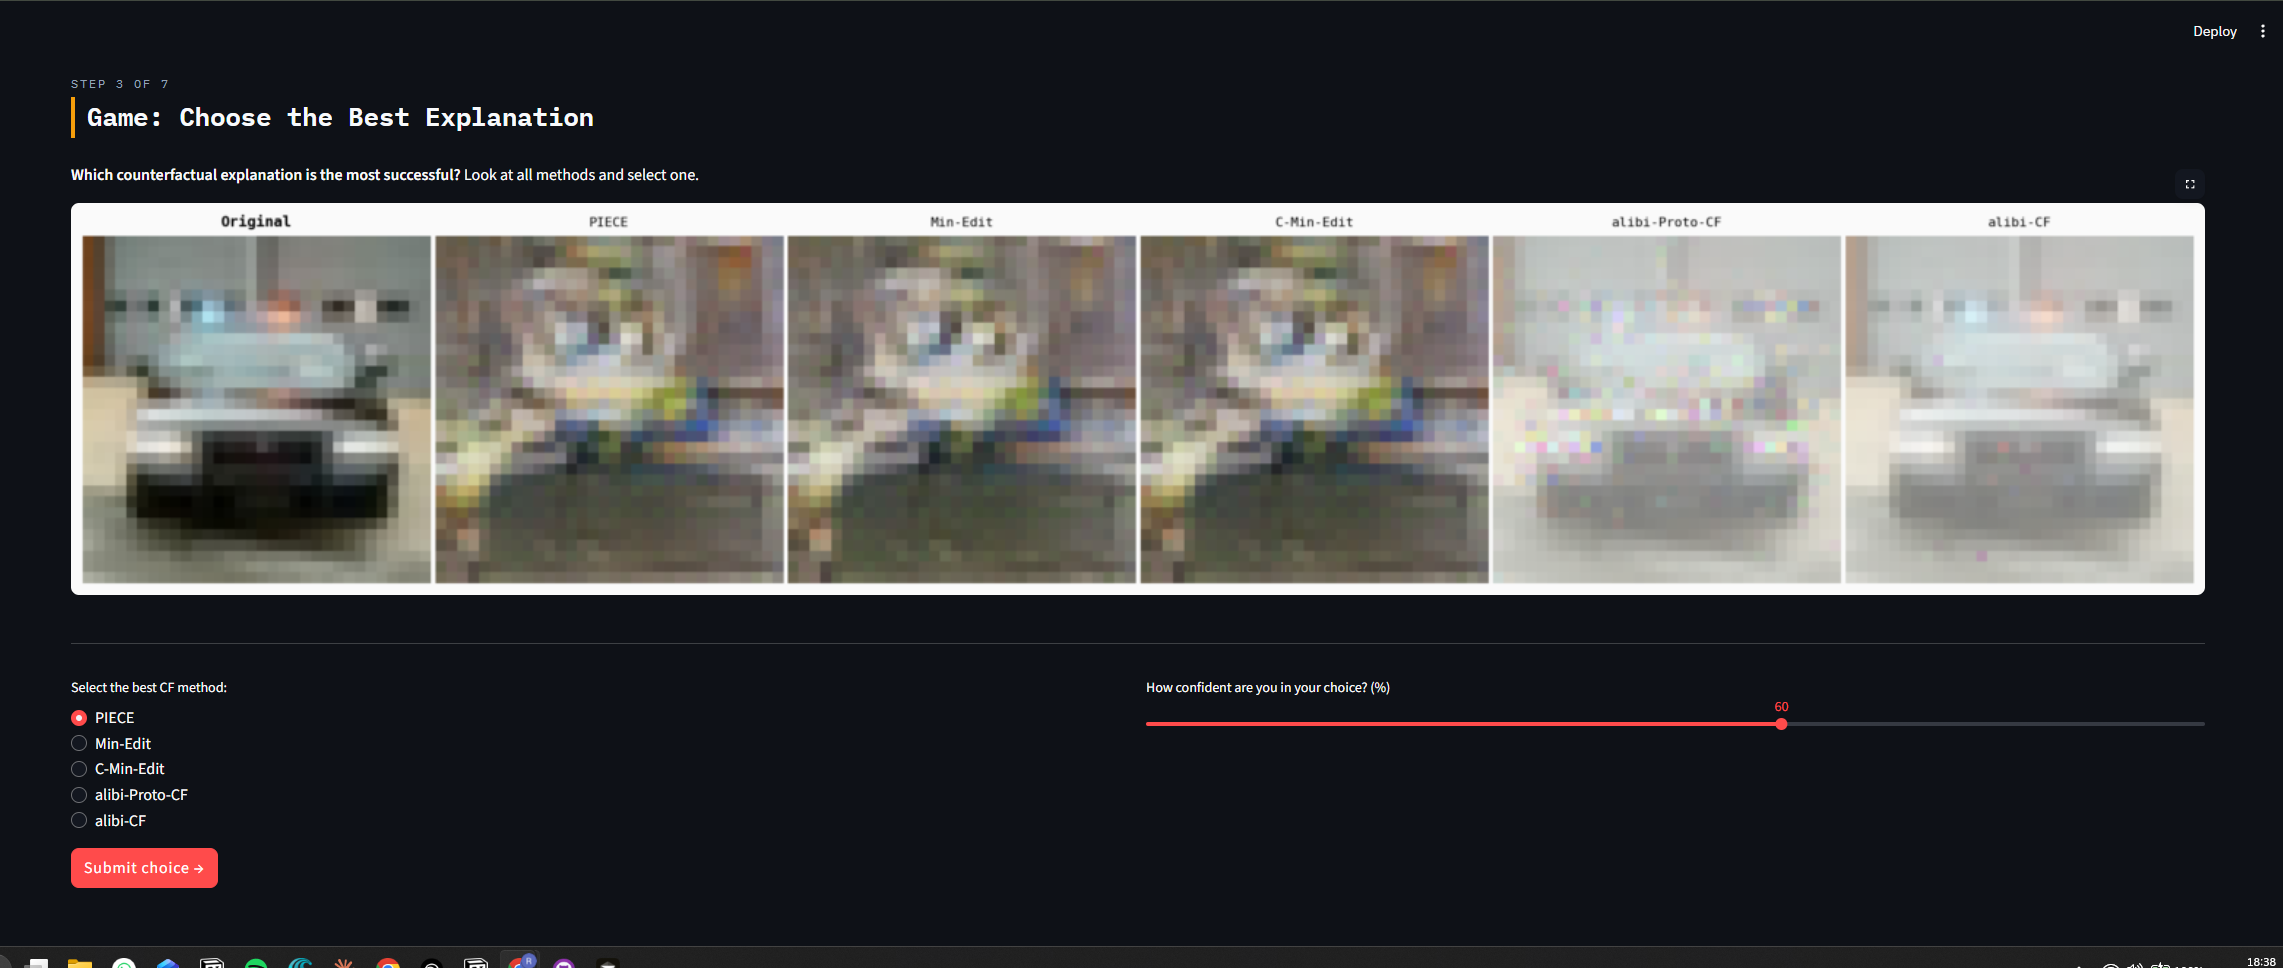
\includegraphics[keepaspectratio]{images/Game choose the best explanation(4).png}}

}

\caption{\label{fig-game}The Game}

\end{figure}%

\begin{figure}

\centering{

\pandocbounded{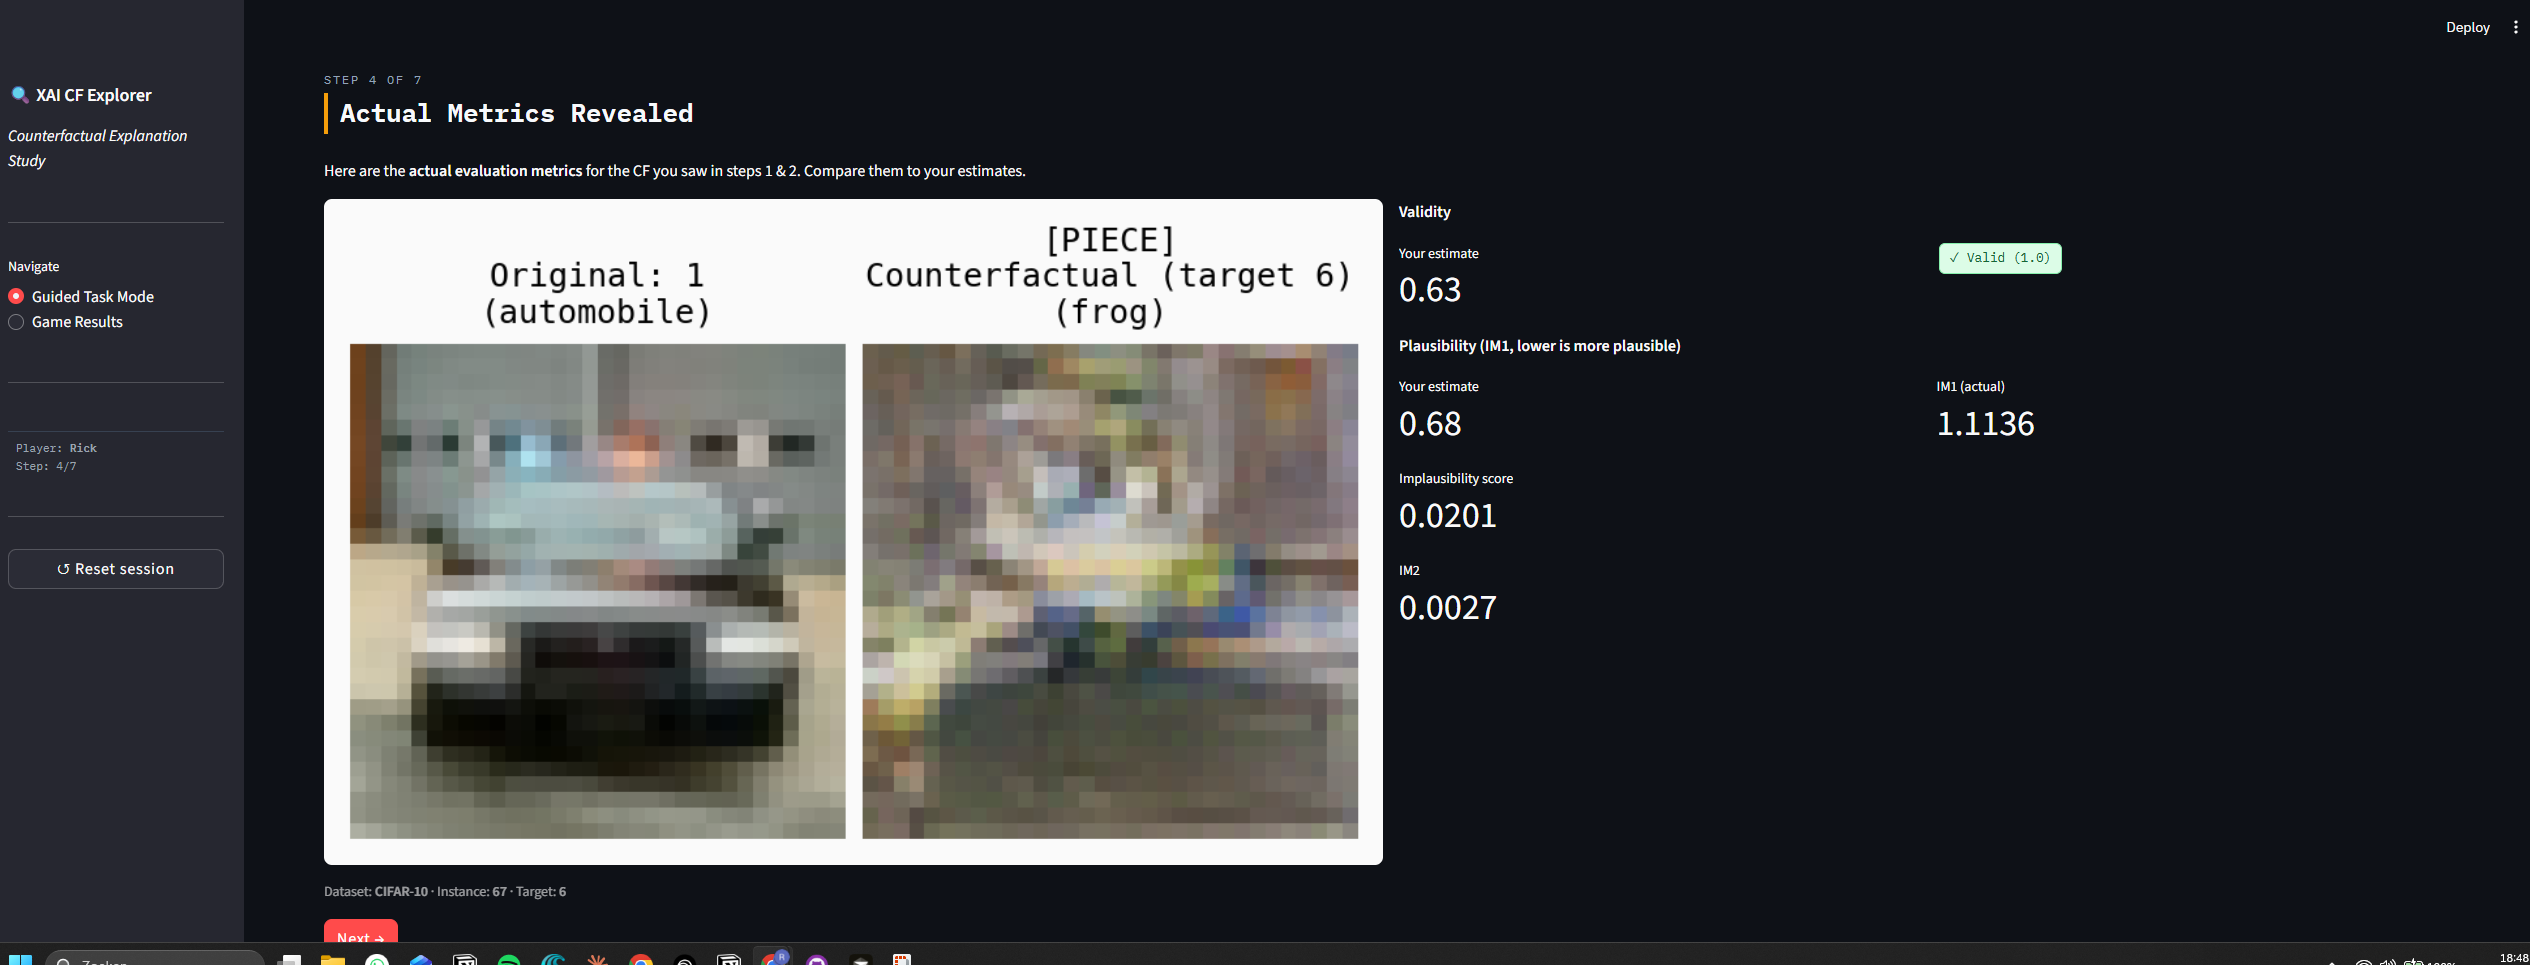
\includegraphics[keepaspectratio]{images/Actual Metrics (5).png}}

}

\caption{\label{fig-metrics}Actual Metrics}

\end{figure}%

\begin{figure}[H]

{\centering \pandocbounded{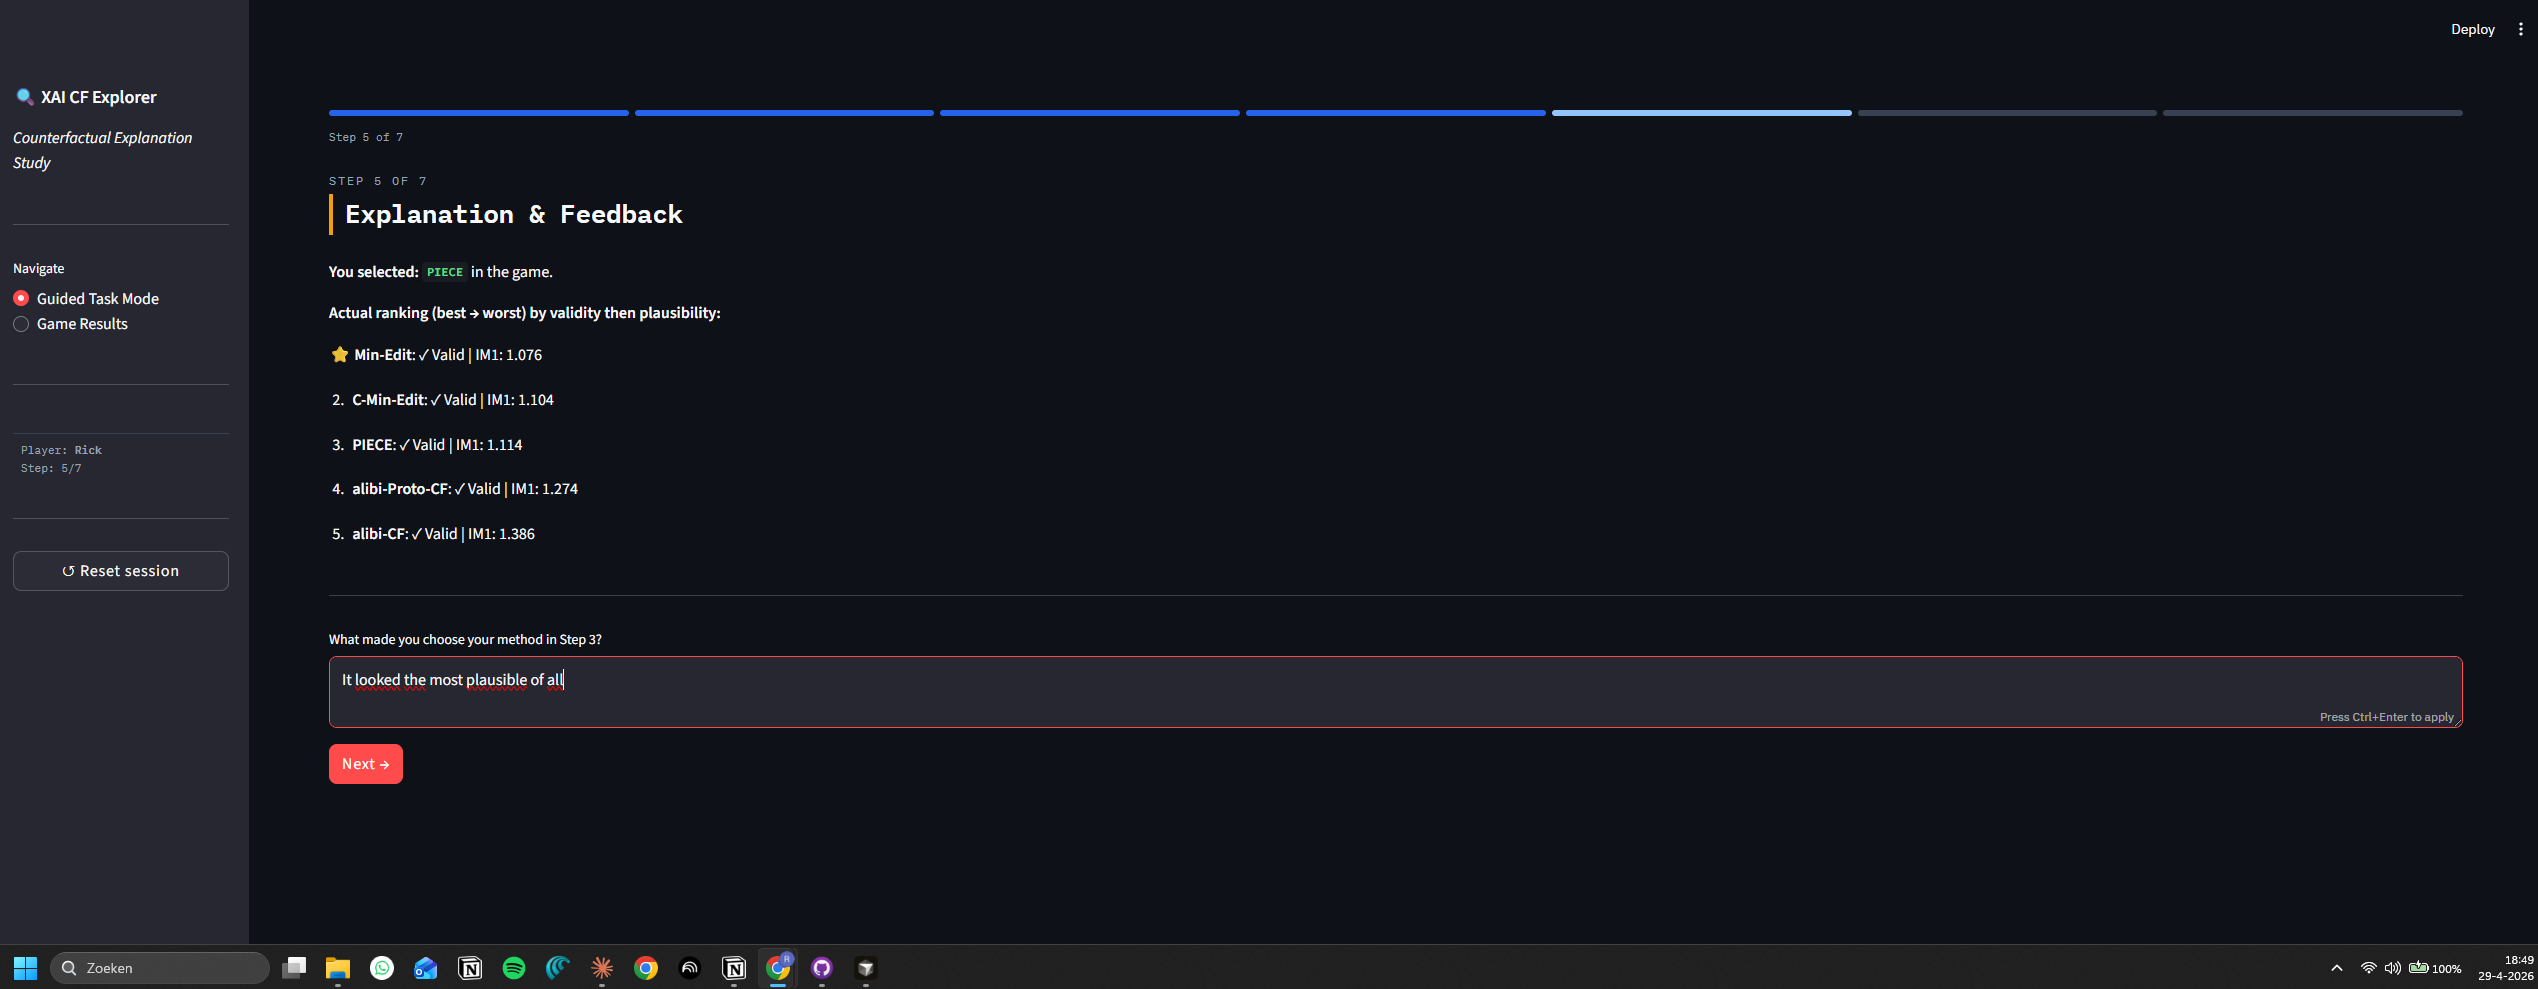
\includegraphics[keepaspectratio]{images/Explanation & Feedback (6).png}}

}

\caption{Explanation \& Feedback}

\end{figure}%

\begin{figure}

\centering{

\pandocbounded{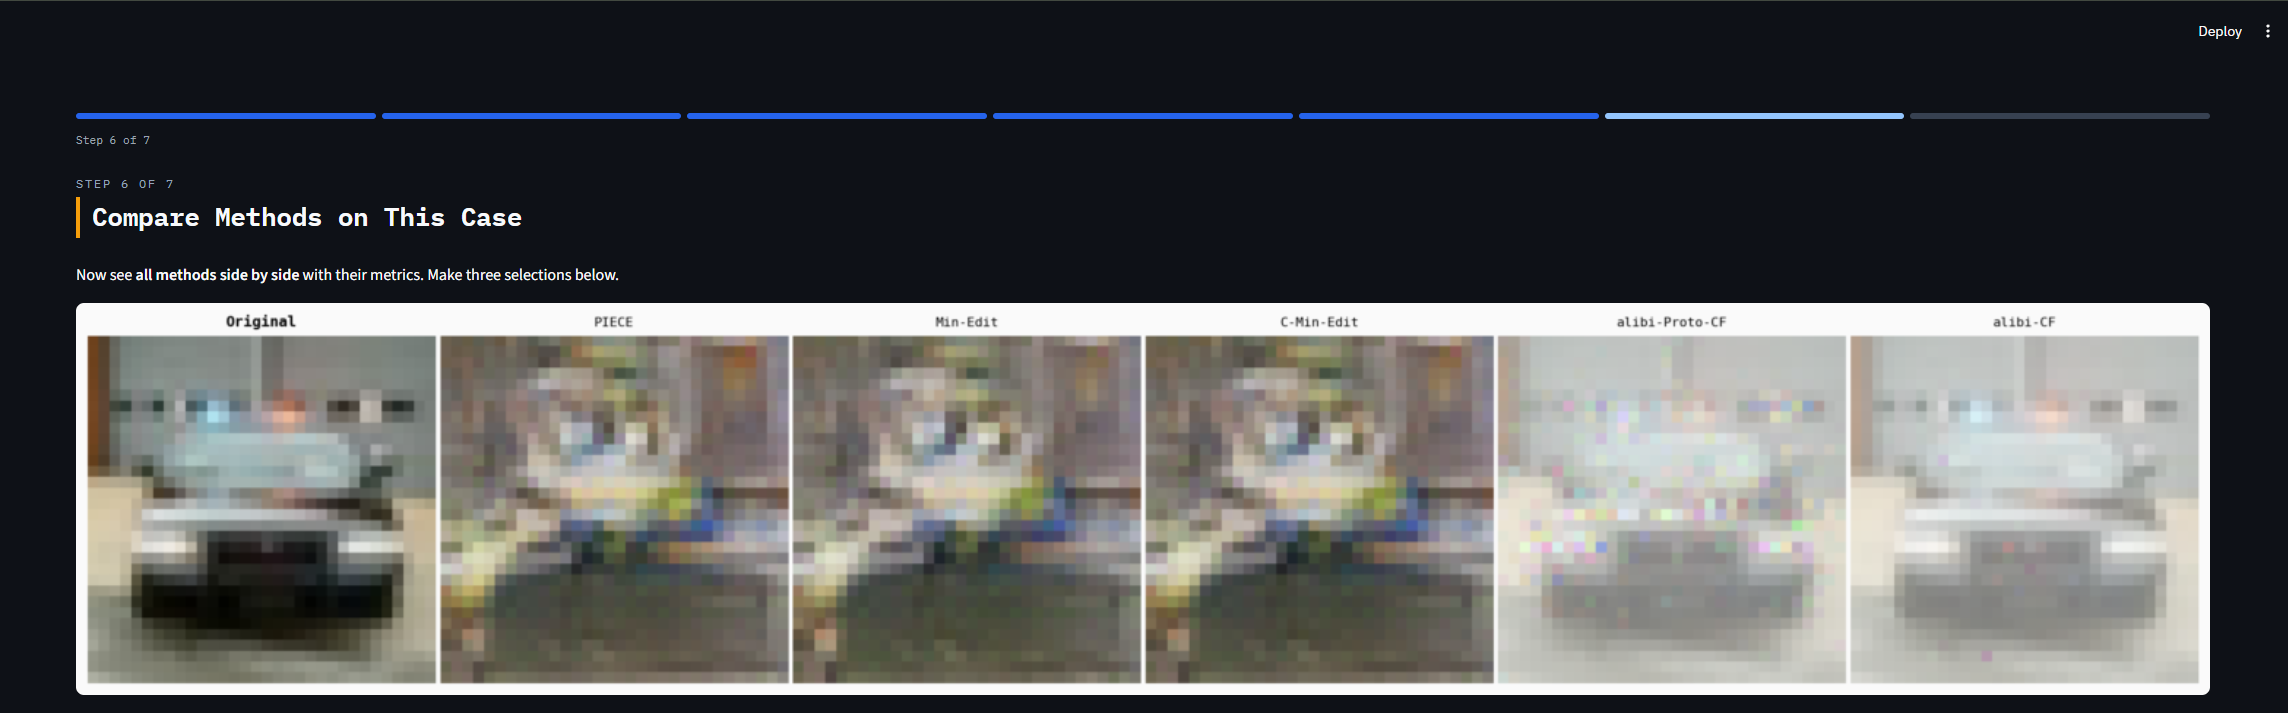
\includegraphics[keepaspectratio]{images/Compare methods on this case (7.1).png}}

}

\caption{\label{fig-compare-methods1}Compare methods 1.1}

\end{figure}%

\begin{figure}

\centering{

\pandocbounded{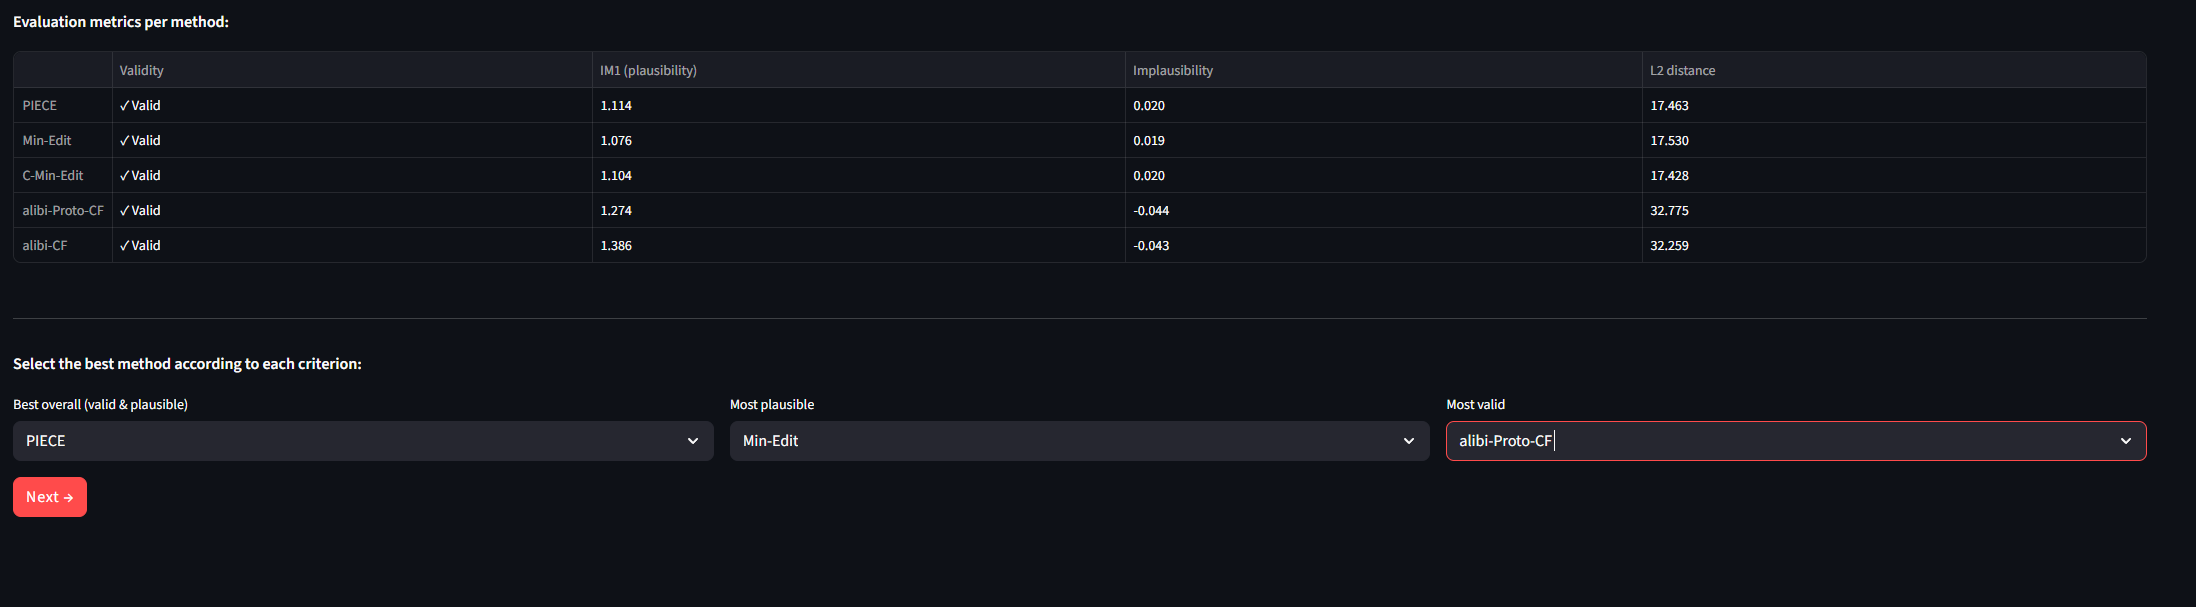
\includegraphics[keepaspectratio]{images/Compare methods on this case (7.2).png}}

}

\caption{\label{fig-compare-methods2}Compare methods 1.2}

\end{figure}%

\begin{figure}

\centering{

\pandocbounded{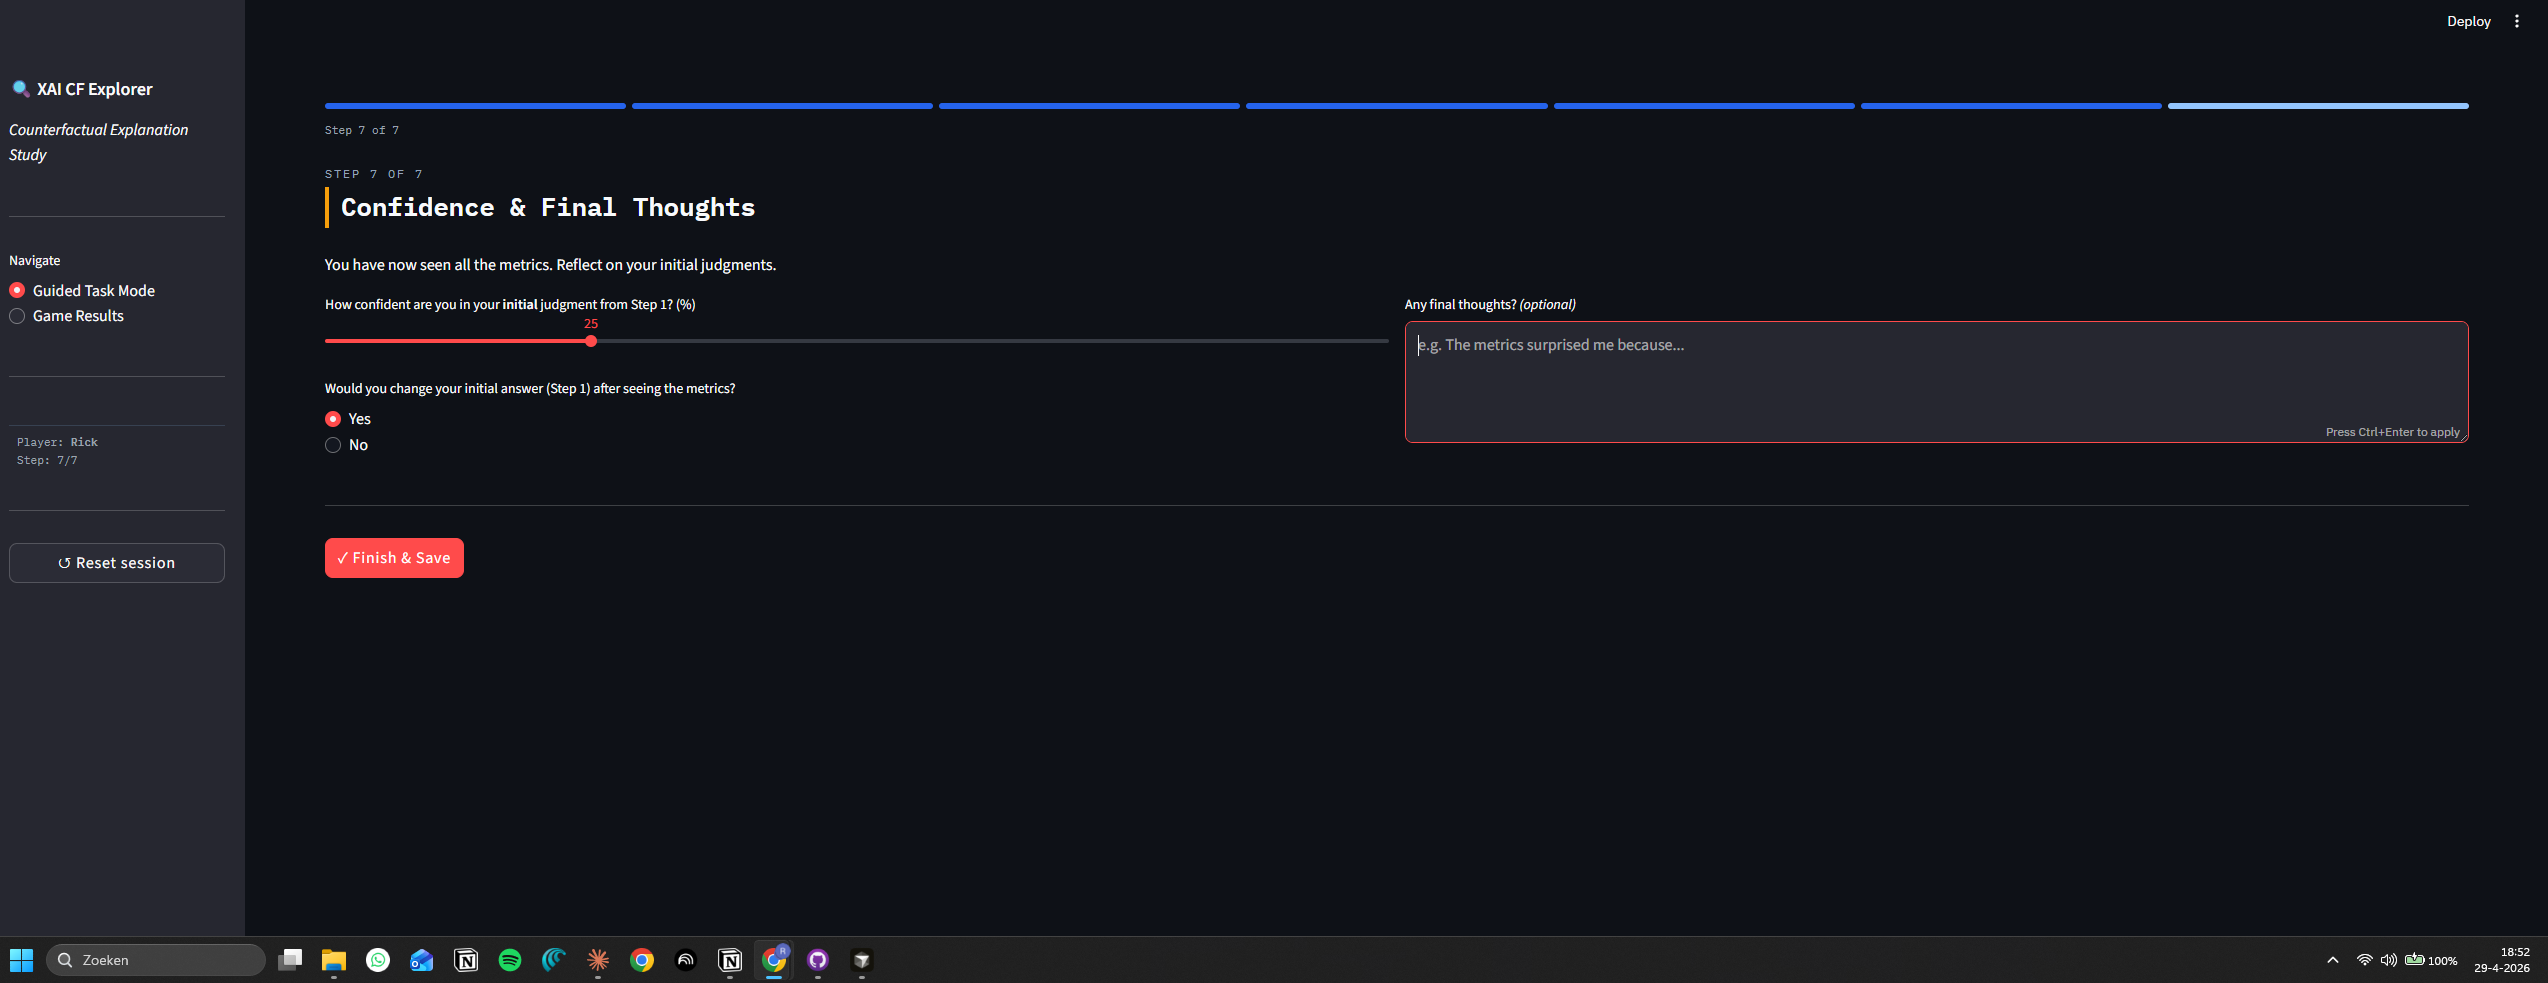
\includegraphics[keepaspectratio]{images/Confidence & Final Thoughts (8).png}}

}

\caption{\label{fig-conclusion}Final Though \& Confidence}

\end{figure}%

\phantomsection\label{refs}
\begin{CSLReferences}{1}{0}
\bibitem[\citeproctext]{ref-amershi2019guidelines}
Amershi, Saleema, Daniel Weld, Mihaela Vorvoreanu, et al. 2019.
{``Guidelines for Human-AI Interaction.''} In \emph{Proceedings of the
2019 CHI Conference}, 1--13.
\url{https://www.microsoft.com/en-us/research/publication/guidelines-for-human-ai-interaction/}.

\bibitem[\citeproctext]{ref-doshivelez2017rigorous}
Doshi-Velez, Finale, and Been Kim. 2017. {``Towards a Rigorous Science
of Interpretable Machine Learning.''} \emph{arXiv Preprint
arXiv:1702.08608}. \url{https://arxiv.org/abs/1702.08608}.

\bibitem[\citeproctext]{ref-guidotti2018survey}
Guidotti, Riccardo, Anna Monreale, Salvatore Ruggieri, Franco Turini,
Fosca Giannotti, and Dino Pedreschi. 2018. {``A Survey of Methods for
Explaining Black Box Models.''} \emph{ACM Computing Surveys} 51 (5):
1--42. \url{https://arxiv.org/abs/1802.01933}.

\bibitem[\citeproctext]{ref-kaur2020interpreting}
Kaur, Harmanpreet, Harsha Nori, Samuel Jenkins, and Rich Caruana. 2020.
{``Interpreting Interpretability: Understanding Data Scientists' Use of
Interpretability Tools for Machine Learning.''} In \emph{Proceedings of
the 2020 CHI Conference}, 1--14. \url{https://arxiv.org/abs/2001.10996}.

\bibitem[\citeproctext]{ref-wachter2017counterfactual}
Wachter, Sandra, Brent Mittelstadt, and Chris Russell. 2017.
{``Counterfactual Explanations Without Opening the Black Box: Automated
Decisions and the GDPR.''} \emph{Harvard Journal of Law \& Technology}
31 (2): 841--87. \url{https://arxiv.org/abs/1711.00399}.

\end{CSLReferences}




\end{document}
